\documentclass[applsci,article,submit,pdftex,moreauthors]{Definitions/mdpi} 
% \documentclass[preprints,article,submit,pdftex,moreauthors]{Definitions/mdpi} 
% For posting an early version of this manuscript as a preprint, you may use "preprints" as the journal.
% Changing "submit" to "accept" before posting will remove line numbers.
% Instead of applsci, for a general submission, use "preprints".

% ==================================================

% MDPI internal commands - do not modify
\firstpage{1} 
\makeatletter 
\setcounter{page}{\@firstpage} 
\makeatother
\pubvolume{1}
\issuenum{1}
\articlenumber{0}
\pubyear{2025}
\copyrightyear{2025}
%\externaleditor{Firstname Lastname} % More than 1 editor, please add `` and '' before the last editor name
\datereceived{ } 
\daterevised{ } % Comment out if no revised date
\dateaccepted{ } 
\datepublished{ } 
% \datecorrected{} % For corrected papers: "Corrected: XXX" date in the original paper.
% \dateretracted{} % For retracted papers: "Retracted: XXX" date in the original paper.
\hreflink{https://doi.org/} % If needed use \linebreak
% \doinum{}
% \pdfoutput=1 % Uncommented for upload to arXiv.org
% \CorrStatement{yes} % For updates
% \longauthorlist{yes} % For many authors that exceed the left citation part

% ==================================================

% Add packages and commands here. The following packages are loaded in our class file: fontenc, inputenc, calc, indentfirst, fancyhdr, graphicx, epstopdf, lastpage, ifthen, float, amsmath, amssymb, lineno, setspace, enumitem, mathpazo, booktabs, titlesec, etoolbox, tabto, xcolor, colortbl, soul, multirow, microtype, tikz, totcount, changepage, attrib, upgreek, array, tabularx, pbox, ragged2e, tocloft, marginnote, marginfix, enotez, amsthm, natbib, hyperref, cleveref, scrextend, url, geometry, newfloat, caption, draftwatermark, seqsplit
% cleveref: load \crefname definitions after \begin{document}

\usepackage[utf8]{inputenc}
\usepackage{color}
\usepackage{graphicx}
\usepackage{placeins}
% \usepackage[margin=1in]{geometry}
\usepackage{appendix}
\usepackage{amsmath, amssymb, bm}
\usepackage{multirow}
\usepackage{placeins}
\usepackage{xfrac}
% \usepackage[colorlinks=true, linkcolor=blue, citecolor=blue]{hyperref}
% \usepackage[nameinlink, capitalize]{cleveref}
\usepackage[font=footnotesize, labelfont=bf]{caption}
%\usepackage{subcaption}
\usepackage[version=4]{mhchem}
\usepackage{lineno}
\usepackage{bm}
\usepackage{comment}
\usepackage[T1]{fontenc}
\usepackage{anyfontsize}
\usepackage{subfig}
\newcommand{\?}{\stackrel{?}{=}}

% ==================================================

% Full title of the paper (Capitalized)
\Title{Atomistic Investigation of Plastic Deformation and Dislocation Motion in Uranium Mononitride}

% MDPI internal command: Title for citation in the left column
\TitleCitation{Atomistic Investigation of Plastic Deformation and Dislocation Motion in Uranium Mononitride}

% Author Orchid ID: enter ID or remove command
\newcommand{\orcidauthorA}{0009-0009-5882-3345} % Add \orcidA{} behind the author's name
\newcommand{\orcidauthorB}{0000-0003-1964-1177} % Add \orcidB{} behind the author's name
\newcommand{\orcidauthorC}{0000-0002-4158-0123} % Add \orcidC{} behind the author's name

% Authors, for the paper (add full first names)
\Author{Mohamed AbdulHameed$^{1}$\orcidA{}, Benjamin Beeler $^{1,2,*}$\orcidB{}, and Antoine Claisse $^{3}$\orcidC{}}

% \longauthorlist{yes}

% MDPI internal command: Authors, for metadata in PDF
\AuthorNames{Mohamed AbdulHameed, Benjamin Beeler, and Antoine Claisse}

% MDPI internal command: Authors, for citation in the left column, only choose below one of them according to the journal style

% If this is a ACS style journal (Except for the above Chicago and APA journals, all others are in the ACS format): 
% Lastname, F.; Lastname, F.; Lastname, F.
\isAPAStyle{%
       \AuthorCitation{AbdulHameed, M., Beeler, B., \& Claisse, A.}
         }{%
        \isChicagoStyle{%
        \AuthorCitation{Mohamed AbdulHameed, Benjamin Beeler, and Antoine Claisse.}
        }{
        \AuthorCitation{AbdulHameed, M.; Beeler, B.; Claisse, A.}
        }
}

% Affiliations / Addresses (Add [1] after \address if there is only one affiliation.)
\address{%
$^{1}$ \quad Department of Nuclear Engineering, North Carolina State University, Raleigh, NC 27695, USA\\
$^{2}$ \quad Idaho National Laboratory, Idaho Falls, ID 83415, USA\\
$^{3}$ \quad Westinghouse Electric Sweden, Västerås, SE 72163, Sweden}

% Contact information of the corresponding author
\corres{Corresponding author: bwbeeler@ncsu.edu}

\abstract{Uranium mononitride (UN) is a promising advanced nuclear fuel due to its high thermal conductivity and high fissile density. However, many aspects of its mechanical behavior, particularly at reactor-relevant conditions, remain unclear. In this study, molecular dynamics (MD) simulations are employed to investigate the deformation behavior and dislocation motion in UN. We found that the Kocevski potential predicts the principal slip system as $\frac{1}{2} \langle 110 \rangle \{110\}$, aligning with experimental data, whereas the Tseplyaev potential predicts slip on $\frac{1}{2} \langle 110 \rangle \{111\}$. MD simulations of stress-strain behavior were used to estimate nanoindentation hardness, revealing that the Kocevski potential accurately predicts hardness even though it fails to model dynamic plasticity. Complete dislocation mobility functions have been fitted for the edge and screw dislocations in both the thermally-activated and phonon-drag regimes. The 300 K linear mobility of the edge dislocation using the Tseplyaev potential was found to be 817 $\mathrm{Pa}^{-1} \! \cdot \! \mathrm{s}^{-1}$, whereas that of the screw dislocation using the Kocevski potential was found to be 4546 $\mathrm{Pa}^{-1} \! \cdot \! \mathrm{s}^{-1}$. At intermediate stresses, we observed that the subsonic steady-state motion of the edge dislocation in UN is intermittently interrupted by velocity jumps, reaching the average sound velocity. Finally, the threshold Schmid stress is calculated as 179--197 MPa, which gives an upper-limit estimate of the uniaxial yield stress of polycrystalline UN of 548--603 MPa. These findings, including the fitted dislocation mobility function, provide essential input for future plasticity and dislocation dynamics models of nuclear fuels.}

% Keywords
\keyword{uranium nitride; molecular dynamics; plastic deformation; stress-strain curve; nanoindentation hardness; Peierls stress; dislocation mobility; critical resolved shear stress} 

% ==================================================

% Only for the journal Applied Sciences
% \featuredapplication{Authors are encouraged to provide a concise description of the specific application or a potential application of the work. This section is not mandatory.}

% ==================================================

\begin{document}

\section{Introduction}

Uranium mononitride (UN) is a promising advanced nuclear fuel for its many attractive characteristics including high uranium density, high thermal conductivity, good chemical compatibility with most potential cladding materials, and longer fuel residence time \cite{Ekberg2018, Wallenius2020, Uno2020}. However, it suffers from some drawbacks including complicated fabrication processes, high fuel cost owing to the need for $^{15}$N enrichment, and low resistance to oxidation by high-temperature steam \cite{Ekberg2018, Wallenius2020, Uno2020}. Many aspects of the behavior of UN under high temperatures and/or irradiation are lacking in both consistent experimental data and detailed mechanistic understanding. The mechanical properties of nuclear fuels are crucial for a better understanding of the pellet-cladding mechanical interactions (PCMI) that occur during reactor operation. The mechanical aspects relevant to PCMI in UN include deformation behavior (stress-strain) and dislocation properties.

% Stress-strain behavior and dislocations

Molecular-dynamics (MD) simulations of the deformation behavior have been conducted for many materials including Si and SiC \cite{Ivashchenko2007}, Al \cite{Li2020}, and Cu \cite{Hansson2022}. Due to the size limitation of MD simulations, most of these studies are of a descriptive nature, except for those studies that specifically target nano-material applications and for which the MD size is representative. To the best of our knowledge, no computational studies of the stress-strain behavior of UN exist in the open literature. The only experimental study found in the literature on the deformation behavior in UN is by Sole and van der Walt \cite{Sole1968}. They observed that the majority of slip traces on UN samples exist within the $\{110\}$ planes, which implies that $\frac{1}{2} \langle 110 \rangle \{110\}$ are the primary slip planes in UN. They also report that most of the dislocations observed are nearly pure screw dislocations. A secondary slip system along the $\{112\}$ planes has been observed by the authors who hypothesized a process for its occurrence that is based on the reaction of two screw dislocations to form an edge dislocation confined to the (112) plane. However, the mechanism by which this edge dislocation slips remains unclear.

Another study was conducted on dislocations in UN by Xiu \textit{et al.} \cite{Xiu2021} who investigated dislocation loops in the proton-irradiated U-N-O system. They stated that only $\frac{a}{2} \langle 110 \rangle$ dislocation loops can be observed in the UN phase. They also conducted 0 K molecular statics using the Tseplyaev and Starikov angular-dependent potential \cite{Tseplyaev2016} to determine the formation energies of $\frac{a}{2} \langle 110 \rangle$ and $\frac{a}{3} \langle 111 \rangle$ dislocation loops at various loop sizes. However, as shown previously \cite{AbdulHameed2024} and verified in this study, 0 K calculations using the Tseplyaev and Starikov angular-dependent potential \cite{Tseplyaev2016} of defective UN structures can be trapped at metastable states and should be treated cautiously. 

Nucleation of dislocations is a primary product of radiation damage in nuclear materials. Knowledge of dislocation mobility is essential to model glide-controlled creep accurately \cite{Skelton2017}. Osetsky and Bacon \cite{Osetsky2003} have introduced a fully atomistic formalism to calculate the Peierls stress and applied it to straight edge dislocations in BCC Fe. Alternatively, a hybrid continuum-atomistic approach based on the Peierls-Nabarro theory has been used by Liu \textit{et al.} \cite{Liu2012} to calculate the Peierls stresses and core widths for NaCl and LiF and by Skelton and Walker \cite{Skelton2017} to calculate the same parameters for \ce{UO2}. Many studies have looked at the dislocation mobility in metals like Al \cite{Cho2017, Dang2019} and Ni \cite{Olmsted2005}, as well as in Al-Mg alloys \cite{Olmsted2005} and steels \cite{Kaloni2023}. Additionally, Yadav \textit{et al.} \cite{Yadav2014} conducted a density functional theory (DFT) study of dislocations in TiN and determined the principal slip system. Ukita \textit{et al.} \cite{Ukita2018} conducted a similar DFT study for NaCl and AgCl.

Two promising interatomic potentials of UN exist in the literature: Tseplyaev and Starikov's angular-dependent potential \cite{Tseplyaev2016}, and Kocevski \textit{et al.}'s embedded-atom method (EAM) potential \cite{Kocevski2022II}. Both potentials have been assessed in our previous work \cite{AbdulHameed2024}, however, their ability to model the dynamical processes of plastic deformation, e.g., dislocation slip and mobility is also worthy of study. This is especially valuable for nuclear fuels where studying the deformation behavior of single crystals provides a baseline to develop a multi-scale modeling approach that can predict the macroscopic mechanical behavior of polycrystalline samples from elementary atomistic mechanisms.

In this work, we perform MD simulations of the stress-strain behavior of nanocrystalline UN. The dynamic processes of plastic deformation as well as the principal slip systems in UN are discussed. The Peierls stress, threshold Schmid stress, and dislocation mobility are computed for straight edge and screw dislocations in UN, and complete mobility functions are fitted. Finally, the yield stress is estimated based on two different approaches.

\section{Computational Methods}

All MD calculations performed in this work utilize the Large-scale Atomic/Molecular Massively Parallel Simulator (LAMMPS) software package \cite{Thompson2022} with a time step of 1 fs and the Tseplyaev \cite{Tseplyaev2016} and Kocevski \cite{Kocevski2022II} potentials. The OVITO software package \cite{Stukowski2010} is used for supercell visualization and analysis.

\subsection{Deformation behavior}

In this paper, we investigate the stress-strain behavior of UN single crystals at $T$ = 300 K and strain rates of $10^8$, $5 \times 10^8$, and $10^9$ s$^{-1}$ using both the Tseplyaev and Kocevski potentials. Due to computational limitations, MD simulations of uniaxial tension are limited to nanometer-sized supercells and strain rates of at least $10^7$ s$^{-1}$ \cite{Lao2013}. $150 \times 30 \times 30$ UN supercells are first equilibrated at 300 K and zero pressure for 100 ps using a Nosé-Hoover thermostat-barostat. After equilibration, the load is applied in the [100] direction at the target strain rate, and the material is allowed to deform in the \textit{NPT} ensemble up to fracture. Periodic boundary conditions (PBCs) were applied in all directions throughout the whole simulation. Relaxation was conducted such that the $x$, $y$, and $z$ directions are independent, but the supercell is ensured to remain orthogonal. Note that during deformation, the $x$ direction is controlled by the strain rate.

To estimate the nanoindentation hardness, we performed deformation simulations at strain rates of $10^7$, $10^8$, and $10^9$ s$^{-1}$ but with PBCs applied only along the loading direction, i.e., the $x$-axis, whereas surfaces perpendicular to the $y$- and $z$-axes are modeled with fixed boundary conditions, yielding free surfaces along these planes. Before deformation, the supercells are equilibrated in the \textit{NPT} ensemble for 50 ps (where the pressure was allowed to equilibrate only along the $x$-axis), and then in the \textit{NVT} ensemble for a further 50 ps. Uniaxial tension was then applied in the \textit{NVT} ensemble until fracture. From the stress-strain curves of nanocrystalline samples with free surfaces, the nanoindentation hardness can be estimated by measuring the stress-strain curves at different strain rates, recording the maximum stress, $\sigma_\mathrm{max}$, at each case, and then extrapolating $\sigma_\mathrm{max}(\Dot{\epsilon})$ to $\Dot{\epsilon} \rightarrow 0$ \cite{Ivashchenko2007}. The linearly extrapolated value should correspond to the experimental nanoindentation hardness values.

We define the maximum stress in the deformation process as the yield stress. Young's modulus is obtained by fitting the linear part of the stress-strain curve excluding the transient at the origin and the non-linearities near the yield point. The Young's modulus along the [100] direction can also be calculated from the elastic constants according to the formula \cite{Rosler2007}:
\begin{equation}
E_{\langle 100 \rangle} = \frac{(C_{11}-C_{12}) \times (C_{11}+2 C_{12})}{C_{11}+C_{12}}
\label{Eq:E100}
\end{equation}

% Also, the anisotropy factor is calculated from \cite{Meyers2009}:
% \begin{equation}
% A = \frac{2 C_{44}}{C_{11} - C_{12}}
% \label{Eq:A}
% \end{equation}

To monitor structural development during deformation, the centrosymmetry parameter (CSP) has been calculated by OVITO for snapshots of the simulated supercells using the minimum-weight matching algorithm \cite{Larsen2020}. The CSP is a measure of the lattice disorder and is defined according to \cite{Kelchner1998}:
\begin{equation}
\mathrm{CSP} = \sum_{i=1}^{N/2} |\mathbf{r}_i + \mathbf{r}_{i+N/2}|^{2} 
\end{equation}
where $N$ is the number of nearest neighbors surrounding an atom ($N$ = 6 for the NaCl crystal structure), and $\mathbf{r}_i$ and $\mathbf{r}_{i+N/2}$ are two vectors from the atom under consideration to a pair of opposite neighbor atoms. For an ideally centrosymmetric crystal, the contributions of all neighbor pairs cancel, and the resulting CSP is zero. The CSP algorithm is robust against thermal fluctuations; for a single crystal, it shows a single peak that starts at zero and whose width increases with increasing $T$. A second peak in the CSP plot corresponds to a different local environment, e.g., dislocations and highly disordered GBs \cite{Bulatov2006, Larsen2020}. The CSP has dimensions of squared distance and is usually given in units of $a^2$, where $a$ is the lattice parameter. The CSP algorithm is an indirect characterization technique. To directly visualize and analyze dislocations, OVITO's dislocation extraction algorithm (DXA) \cite{Stukowski2012} is utilized, and applied to the U sub-lattice. A limitation of the DXA is that it can only identify predefined dislocations in single-component crystals so that dislocations with a Burgers vector that does not belong to any of the predefined families are not identified. This prohibits the algorithm from identifying grain boundary (GB) dislocations that have much shorter Burgers vectors than those of lattice dislocations \cite{Cai2016}. Since each sub-lattice in the B1 structure of UN is a face-centered cubic (FCC) lattice, by applying the DXA to the U sub-lattice we can accurately visualize dislocations. 

\subsection{Dislocation motion}

Ionic crystals have a Burgers vector $\mathbf{b} = \frac{1}{2} \langle 110 \rangle$ and four possible slip planes: $\{ 110 \}$, $\{ 111 \}$, $\{ 100 \}$, and $\{ 112 \}$; the principal one being determined mainly by the bonding nature \cite{Hull2011, Yadav2014}. Three straight edge dislocations are studied in this paper: $\frac{1}{2} [ 110 ] ( 1 \Bar{1} 0 )$, $\frac{1}{2} [ \Bar{1} 1 0 ] ( 111 )$, and $\frac{1}{2} [ \Bar{1} 10 ] ( \Bar{1} \Bar{1} 2 )$ where their Burgers vectors are along the $x$-axis and line vectors along the $z$-axis. To construct an edge dislocation, two half-crystals are stacked on top of one another--the top half-crystal containing one extra atomic plane compared to the bottom half-crystal. Then, strains of $-0.5b/l_x$ and $+0.5b/l_x$ are applied to the top and bottom crystals, respectively, $l_x$ being the length of the respective half-crystal along the $x$-axis \cite{Osetsky2003}. That is, the top half-crystal is compressed by $b/2$ and the bottom half-crystal is stretched by $b/2$. Up to this point, only a misfit dislocation with a zero Burgers vector is formed \cite{Osetsky2003}. To convert it into a perfect edge dislocation, the supercell energy was minimized at 0 K using a nonlinear conjugate gradient method with a minimum relative energy tolerance of $10^{-13}$. This construction method allows to maintain periodicity along the slip direction of the edge dislocation and naturally resolves the anisotropic features of the dislocation core.

A $\frac{1}{2} [ 110 ] ( \Bar{1} 1 0 )$ screw dislocation is constructed by Atomsk using the Volterra construction method of the isotropic elasticity theory \cite{Hull2011}. Periodicity is recovered along the slip direction by tilting the supercell vector parallel to the glide direction by $b/2$. This is achieved in Atomsk by adding a $z$-component equal to $b/2$ to the $x$-vector of the supercell. Then, the supercell energy is minimized at 0 K to resolve the anisotropic features of the dislocation core.

It should be emphasized that all atoms are assumed neutral and charge neutrality is maintained for all supercells containing dislocations. Charge effects are often associated with dislocations in ionic crystals \cite{Smoluchowski1966}; however, because it behaves as a metal, defects (including dislocations) in UN have no associated charge and are principally neutral \cite{Cooper2023}.

% If a charged defect existed in a metal, the free electrons in the metal would quickly rearrange themselves to screen and neutralize its charge. Viewed another way, due to the continuity of the electronic band structure in metals, adding an electron (or hole) would not create a stable charged defect because the electron (or hole) would quickly redistribute itself among the available states.

\begin{figure}[h!]
\centering
\subfloat[]{\label{Fig:Qwerty}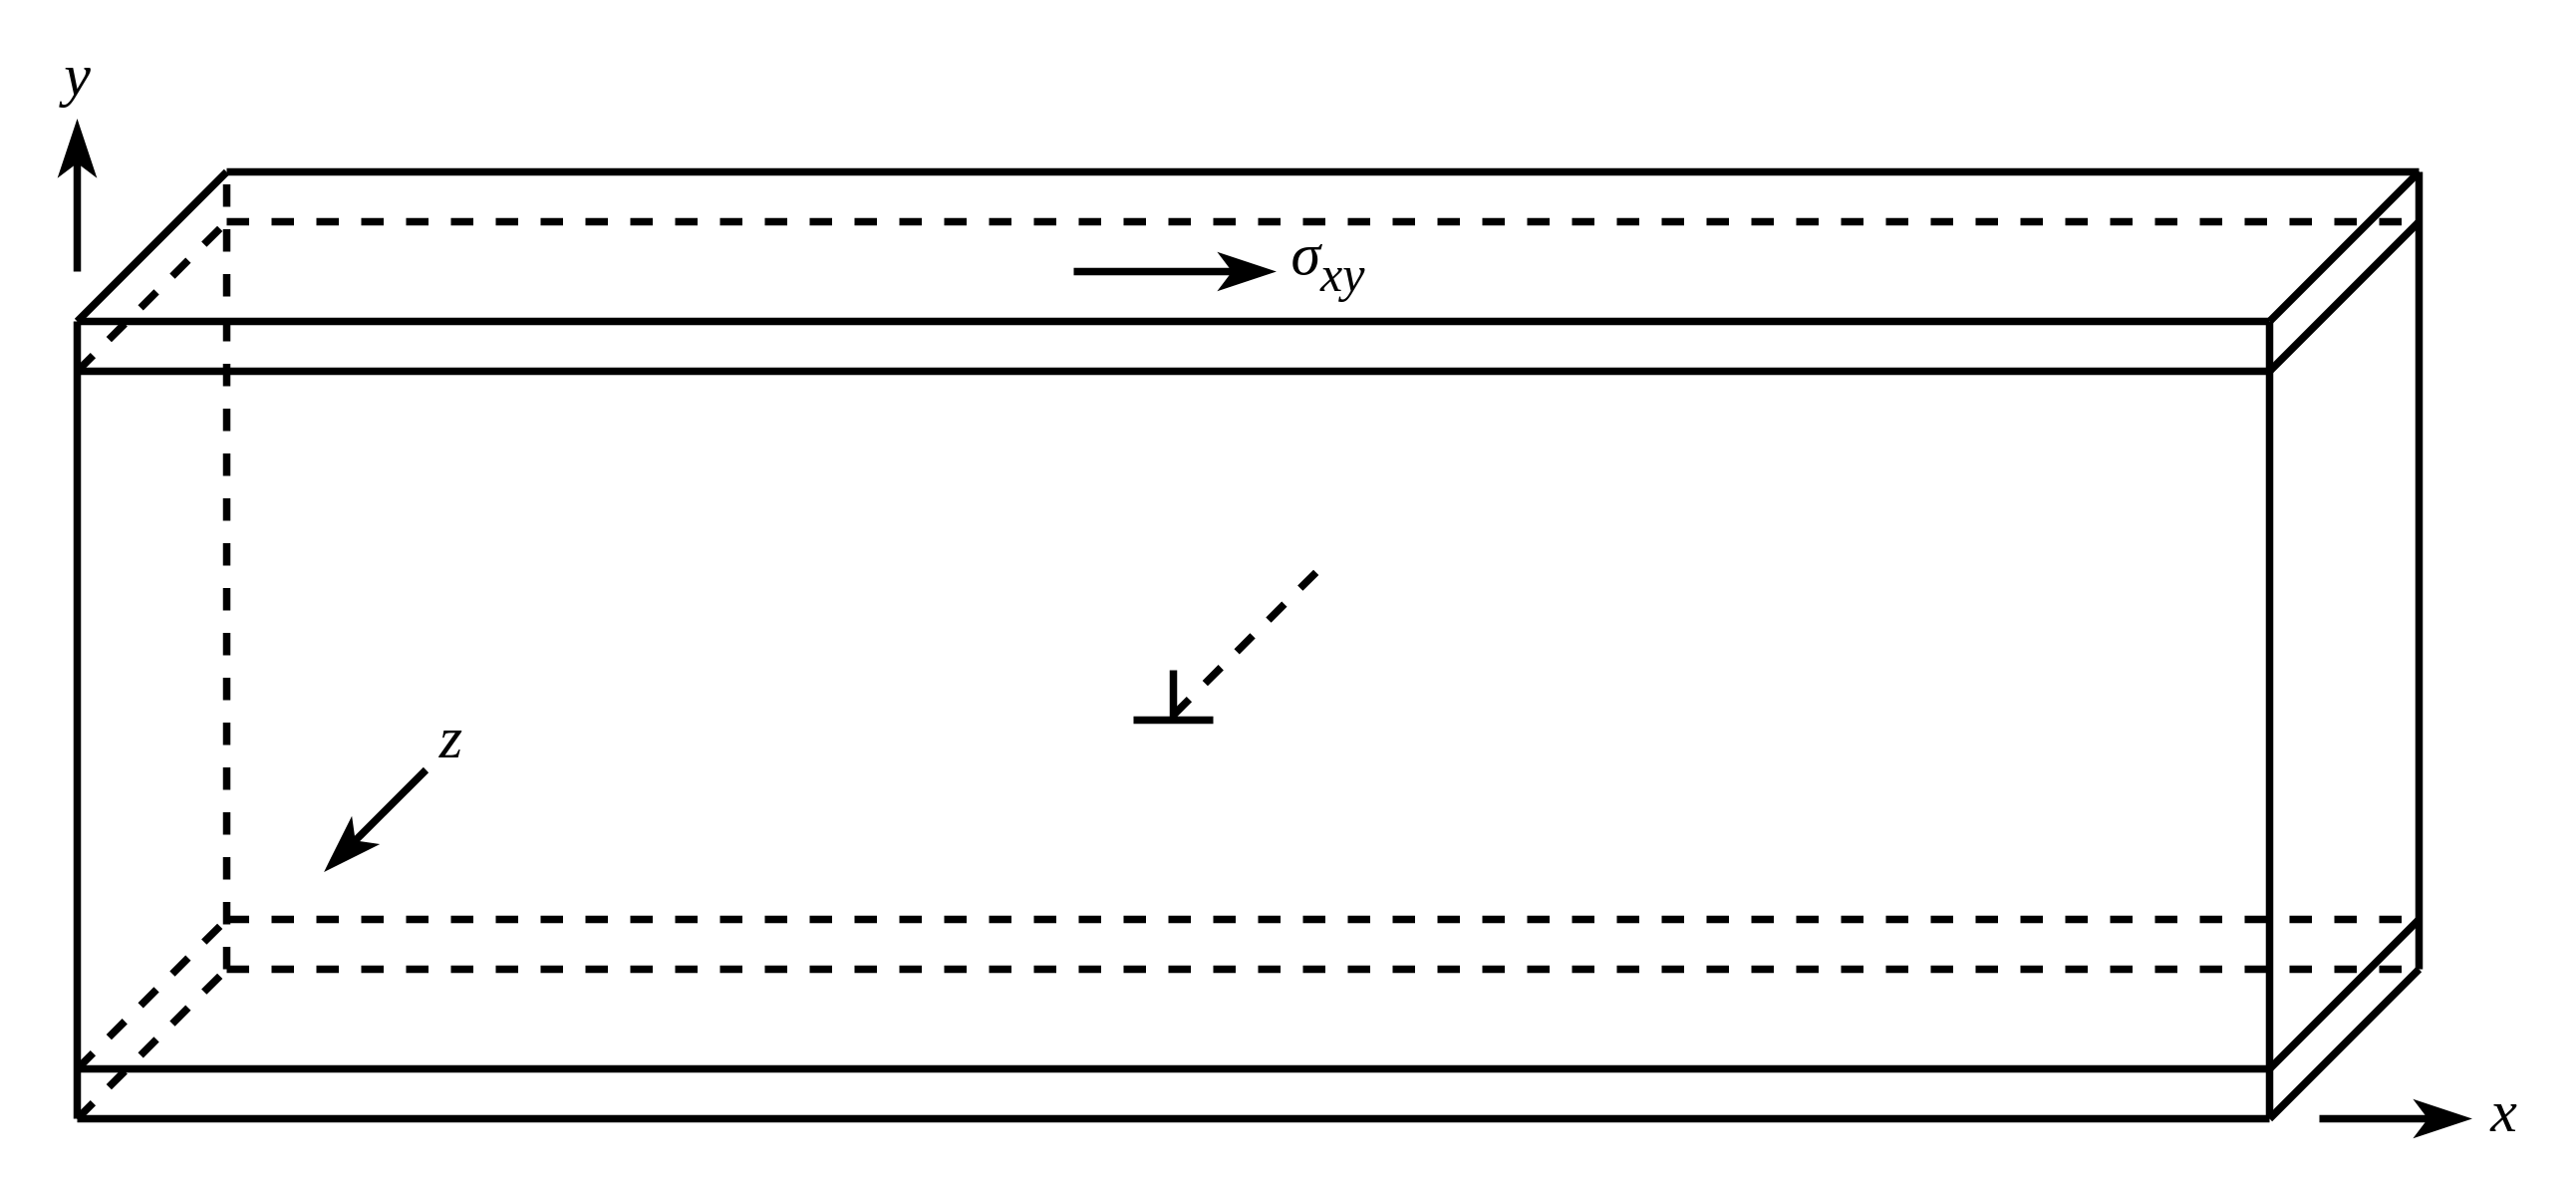
\includegraphics[width=0.48\textwidth]{Qwerty.png}}
\hfill
\subfloat[]{\label{Fig:DislocLine}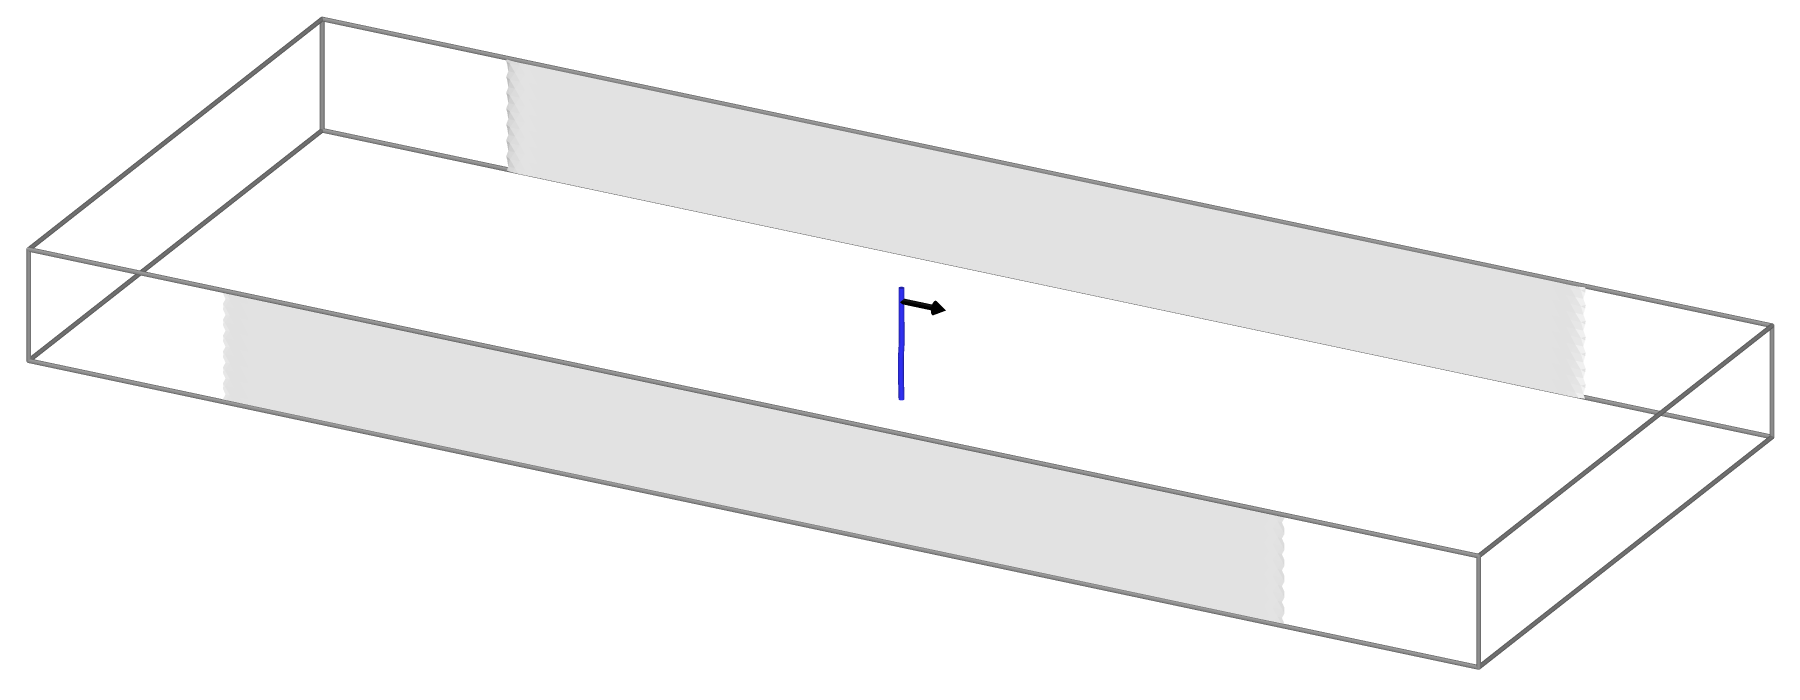
\includegraphics[width=0.48\textwidth]{DislocLine.png}}

\caption{\textbf{(a)} Schematic of the supercell constructed to study straight edge dislocations. For glide along the $\{ 110 \}$ planes, $x = [110]$, $y = [ 1 \Bar{1} 0 ]$, and $z = [001]$. For glide along the $\{ 111 \}$ planes, $x= [ \Bar{1} 1 0 ]$, $y = [111]$, and $z = [ \Bar{1} \Bar{1} 2 ]$. The top layer on which stress/strain is applied as well as the fixed bottom layer are also shown. \textbf{(b)} OVITO visualization of the $\frac{1}{2} [\Bar{1}10] (111)$ edge dislocation and its Burgers vector after equilibration at 1 K. The free surfaces can be identified from the gray ``defect mesh''. In \textbf{(a)} the base plane is the $xz$ plane, whereas in \textbf{(b)} the base plane is the $xy$ plane.}
\label{Fig:DislocStructure}
\end{figure}

For both edge and screw dislocations, the simulation environment for the 0 K minimization is set up as follows (see \cref{Fig:DislocStructure} for a schematic representation for the edge dislocation): PBCs are implemented in the $x$- and $z$-directions, which are the dislocation line direction and slip direction, respectively, while a fixed boundary condition is applied in the $y$-direction. Atoms in the top layer, whose thickness was arbitrarily chosen as 0.05 $l_y$, are restricted to move in the $xz$ plane, whereas atoms in the bottom layer, whose thickness is also 0.05 $l_y$, are fixed in all directions. Then, a multi-step conjugate-gradient minimization, with a minimum relative energy tolerance of $10^{-13}$, is employed.

For the calculation of the Peierls stress at 1 K, the supercells have approximately the same dimensions: $l_x \approx 550$ \AA, $l_y \approx 200$ \AA, and $l_z \approx 40$ \AA. Similar simulation setups and supercell dimensions have been used elsewhere \cite{Osetsky2003, Olmsted2005, Cho2017, Dang2019, Kaloni2023} where the supercell dimensions along the $x$ and $y$ directions have been chosen to nearly eliminate the effects of the free surfaces and periodic images on the dislocation motion. The line direction, $l_z$, must be long enough to contain a kink pair, yet not too long to contain multiple kinks which would lead to self-pinning \cite{Gilbert2011}.

The Kocevski potential was unable to resolve the initial edge dislocation structure of the misfit dislocation into a perfect edge dislocation with a finite Burgers vector. This occurred despite using energy tolerances as low as $10^{-20}$. The issue likely stems from repulsion between uranium atoms, as the Kocevski potential cannot stabilize metallic uranium \cite{AbdulHameed2024}. As a result, only the Tseplyaev potential was used to study edge dislocations. Both the Kocevski and Tseplyaev potentials could stabilize screw dislocations. However, when simulating the motion of the screw dislocation with the Tseplyaev potential, a trail of vacancy and interstitial clusters continuously form during dislocation movement, even at low stresses. In contrast, the $\frac{1}{2} [110] ( \Bar{1} 1 0 )$ screw dislocation moved smoothly up to about 1125 MPa under the Kocevski potential. Therefore, the screw dislocation was studied exclusively with the Kocevski potential.

The Peierls stress is the applied resolved shear stress that moves a dislocation by at least one Burgers vector without thermal assistance, typically near $T = 0$ K \cite{Hull2011}. This is usually measured under a condition of constant strain increment \cite{Puls1976, Osetsky2003}. However, defining strain increments at 0 K is somewhat artificial. Our previous study \cite{AbdulHameed2024} suggests that the Tseplyaev potential may predict metastable states for UN supercells strained at 0 K. To avoid these issues, we calculate the Peierls stress at $T = 1$ K using both potentials.

After static minimization, the supercell containing a dislocation is equilibrated in the \textit{NVT} ensemble for 50 ps. To eliminate the impact of thermostat friction, the thermostat function is simulated with the \textit{NVE} ensemble coupled to velocity scaling. Once equilibration is complete, velocity scaling is turned off. Shear strain rates $\Dot{\epsilon}_{xy}$ and $\Dot{\epsilon}_{yz}$, both set to $10^{-4}$ s$^{-1}$, are then applied to the top layer of the supercell containing an edge and screw dislocation, respectively. Osetsky and Bacon \cite{Osetsky2003} demonstrated that the Peierls stress is independent of strain rate. The simulation runs for 2 ns, and the stress on the dislocation is measured by averaging the atomic $\sigma_{xy}$ and $\sigma_{yz}$ stresses for edge and screw dislocations, respectively, every 10 ps.

The dislocation mobility function is the essential input parameter in any plasticity or dislocation dynamics model \cite{Kaloni2023}. The dislocation mobility of UN at 300 K is computed by first scaling the relaxed supercells by the ratio of the 0 K and 300 K lattice parameters after relaxation to correct for thermal expansion \cite{Cho2017}. Then, the system is equilibrated at a temperature of 300 K under the \textit{NVE} ensemble coupled to velocity scaling for 50 ps. After equilibration, a shear force is applied to the upper layer of the supercell whose thickness is 0.05 $l_y$. The simulation is run for 1 ns and the position of the moving dislocation is recorded every 10 ps. The calculation has been repeated using 5 different initial velocity distributions for both dislocation types. The shear stress for edge dislocations varies between 25 and 2250 MPa, while for screw dislocations, it ranges from 25 to 1200 MPa, with both cases using a stress increment of 25 MPa.

For all calculations, dislocation motion was tracked using the following methodology: Snapshots of the atomic trajectories of each calculation are processed using OVITO where, for each snapshot, the location of the dislocation is identified using the CSP algorithm. Then, the $x$-coordinate of the dislocation is calculated as the average among the $x$-coordinates of all atoms belonging to the dislocation core. Based on visual inspection and comparison with the DXA applied to the U-sublattice, we found that CSP $\geq$ 2 \AA$^2$ exclusively selects the atoms belonging to the dislocation core. A limitation of this methodology is that it assumes that atoms belonging to the dislocation core only move as a single unity along a single slip plane. For all calculations in this paper, we confirmed by visual inspection that this is indeed the case. However, this methodology can be extended to study, e.g., the cross-slip of screw dislocations by tracking both the $x$- and $y$-coordinates of the dislocation core.

In general, there exist three regimes for dislocation motion depending on the values of the shear stress (or, equivalently the strain rate) and temperature:

(\textit{a}) Regime I: Under very low stresses/temperatures, dislocations move via the kink-pair nucleation mechanism, where the dislocations are nearly straight lines, which suggests the existence of only one kink pair at any given time \cite{Gilbert2011}. Under these circumstances, the dislocation motion is thermally activated, and has an Arrhenius-like dependence on temperature \cite{Gilbert2011, Starikov2020}:
\begin{equation}
v_\text{I} = v_t \sqrt{s} \ \mathrm{exp} \left[ - \frac{H_0}{2 k_B T} \left(1-s^p\right)^q \right]
\label{Eq:MobI}
\end{equation}
where $v_t$ is the velocity corresponding to the transition from the exponential thermally-activated regime (Regime I) to the linear phonon drag regime (Regime II), $s = \tau/\tau_t$ is the shear stress normalized by the transition stress, $\tau_t$, between the two regimes, and $H_0 \left(1-s^p\right)^q$ is the stress-dependent kink-pair nucleation enthalpy, with $H_0$ being the kink-pair formation energy at zero temperature and zero stress. $H_0$ can be calculated from stress-relaxation measurements or molecular statics \cite{Ventelon2009, Gilbert2011}. In this work, however, $H_0$ is treated as a fitting parameter. According to the linear elasticity theory, $p=0.5$ and $q=1.25$ for a sinusoidal potential. For more complex potentials, $p$ and $q$ are treated as fitting parameters, which is our approach in this work, and have the following ranges: $0 \leq p \leq 1$ and $1 \leq q \leq 2$.

(\textit{b}) Regime II: As the temperature and/or stress are increased, kink-pair nucleation and propagation become of comparable rates (i.e., kink-pair nucleation is no longer the rate-limiting step) leading to rough dislocation lines \cite{Gilbert2011}. Under these conditions, the stress is large enough so that there is no thermal barrier to motion, and the velocity varies linearly with stress \cite{Dang2019, Olmsted2005}. This viscous drag mainly arises from dislocation interactions with lattice phonons \cite{Dang2019}. In this regime, the velocity takes the form:
\begin{equation}
v_\text{II} = \frac{b \tau}{B} + C
\label{Eq:MobII}
\end{equation}
where $b$ is the magnitude of Burgers vector, $B$ is the linear drag coefficient, and $C$ is an additive constant that has the units of velocity. The linear dislocation mobility in this regime is calculated as $M = 1/B$.

(\textit{c}) Regime III: Under even higher stresses, the relation between $v$ and $\tau$ becomes nonlinear due to a combination of phonon and radiative damping, and the velocity asymptotically approaches the transverse sound velocity \cite{Dang2019}. Radiative damping arises from the emission (radiation) of waves by dislocations during their motion and is independent of temperature. Although we identify the transition stress, $\tau_t'$, between Regimes II and III, Regime III is not handled in this study, and the fitted mobility function is restricted to Regimes I and II.

% In this regime, the relationship between the shear stress and velocity is expressed as:
% \begin{equation}
% \tau = \frac{1}{b} \left[ B ( v - v_t ) + D ( v - v_t' )^a \right]
% \end{equation}
% where $D$ is the nonlinear drag coefficient, $v_t'$ is a transition velocity between the linear and nonlinear regimes, and the exponent $a$ is traditionally estimated as $a=1.5$ \cite{Eshelby1956}. 

\section{Results}

\subsection{Deformation behavior}
\label{Sec:SS}

The results of the stress-strain computations for single-crystal UN are presented in \cref{Fig:SS}. Additionally, Young's moduli of UN along the [100] direction as calculated by \cref{Eq:E100} using experimental and potential-predicted elastic constants as reported in \cite{Salleh1986} and \cite{AbdulHameed2024}, respectively, are presented in \cref{Tab:E100}. In MD stress-strain simulations, a numerical artifact arises where the stress continues to oscillate around zero after fracture (not shown) due to the interference between the tensile wave and its reflection off the fractured free surface, which results in regions with significant compressive stresses \cite{Wen2022}. The stress-strain curves in \cref{Fig:SS} were truncated before displaying these oscillations. Comparing \cref{Fig:SS-ADP-PBCs,Fig:SS-ADP-FreeSurf} to \cref{Tab:E100}, it can be seen that the small-strain $E_{[100]}$ predicted by the Tseplyaev potential (522.7 GPa) is overestimated compared to the large-strain value extracted from the stress-strain curve (410--430 GPa), which is closer to the experimental value (387 GPa), with the supercell having free surfaces showing the closest agreement. On the contrary, the small-strain $E_{[100]}$ predicted by the Kocevski potential (354.1 GPa, \cref{Tab:E100}) is closer to the experimental value that the large-strain value (300 GPa) as shown in \cref{Fig:SS-EAM-PBCs,Fig:SS-EAM-FreeSurf}. However, both supercells with PBCs and free surfaces have essentially the same Young's modulus. Young’s moduli of nanocrystalline UN are relevant for bulk UN because Young’s modulus is only slightly affected by structural miniaturization \cite{Pal2020}.

\begin{figure}[h!]
\centering
\subfloat[Kocevski potential + Full PBCs]{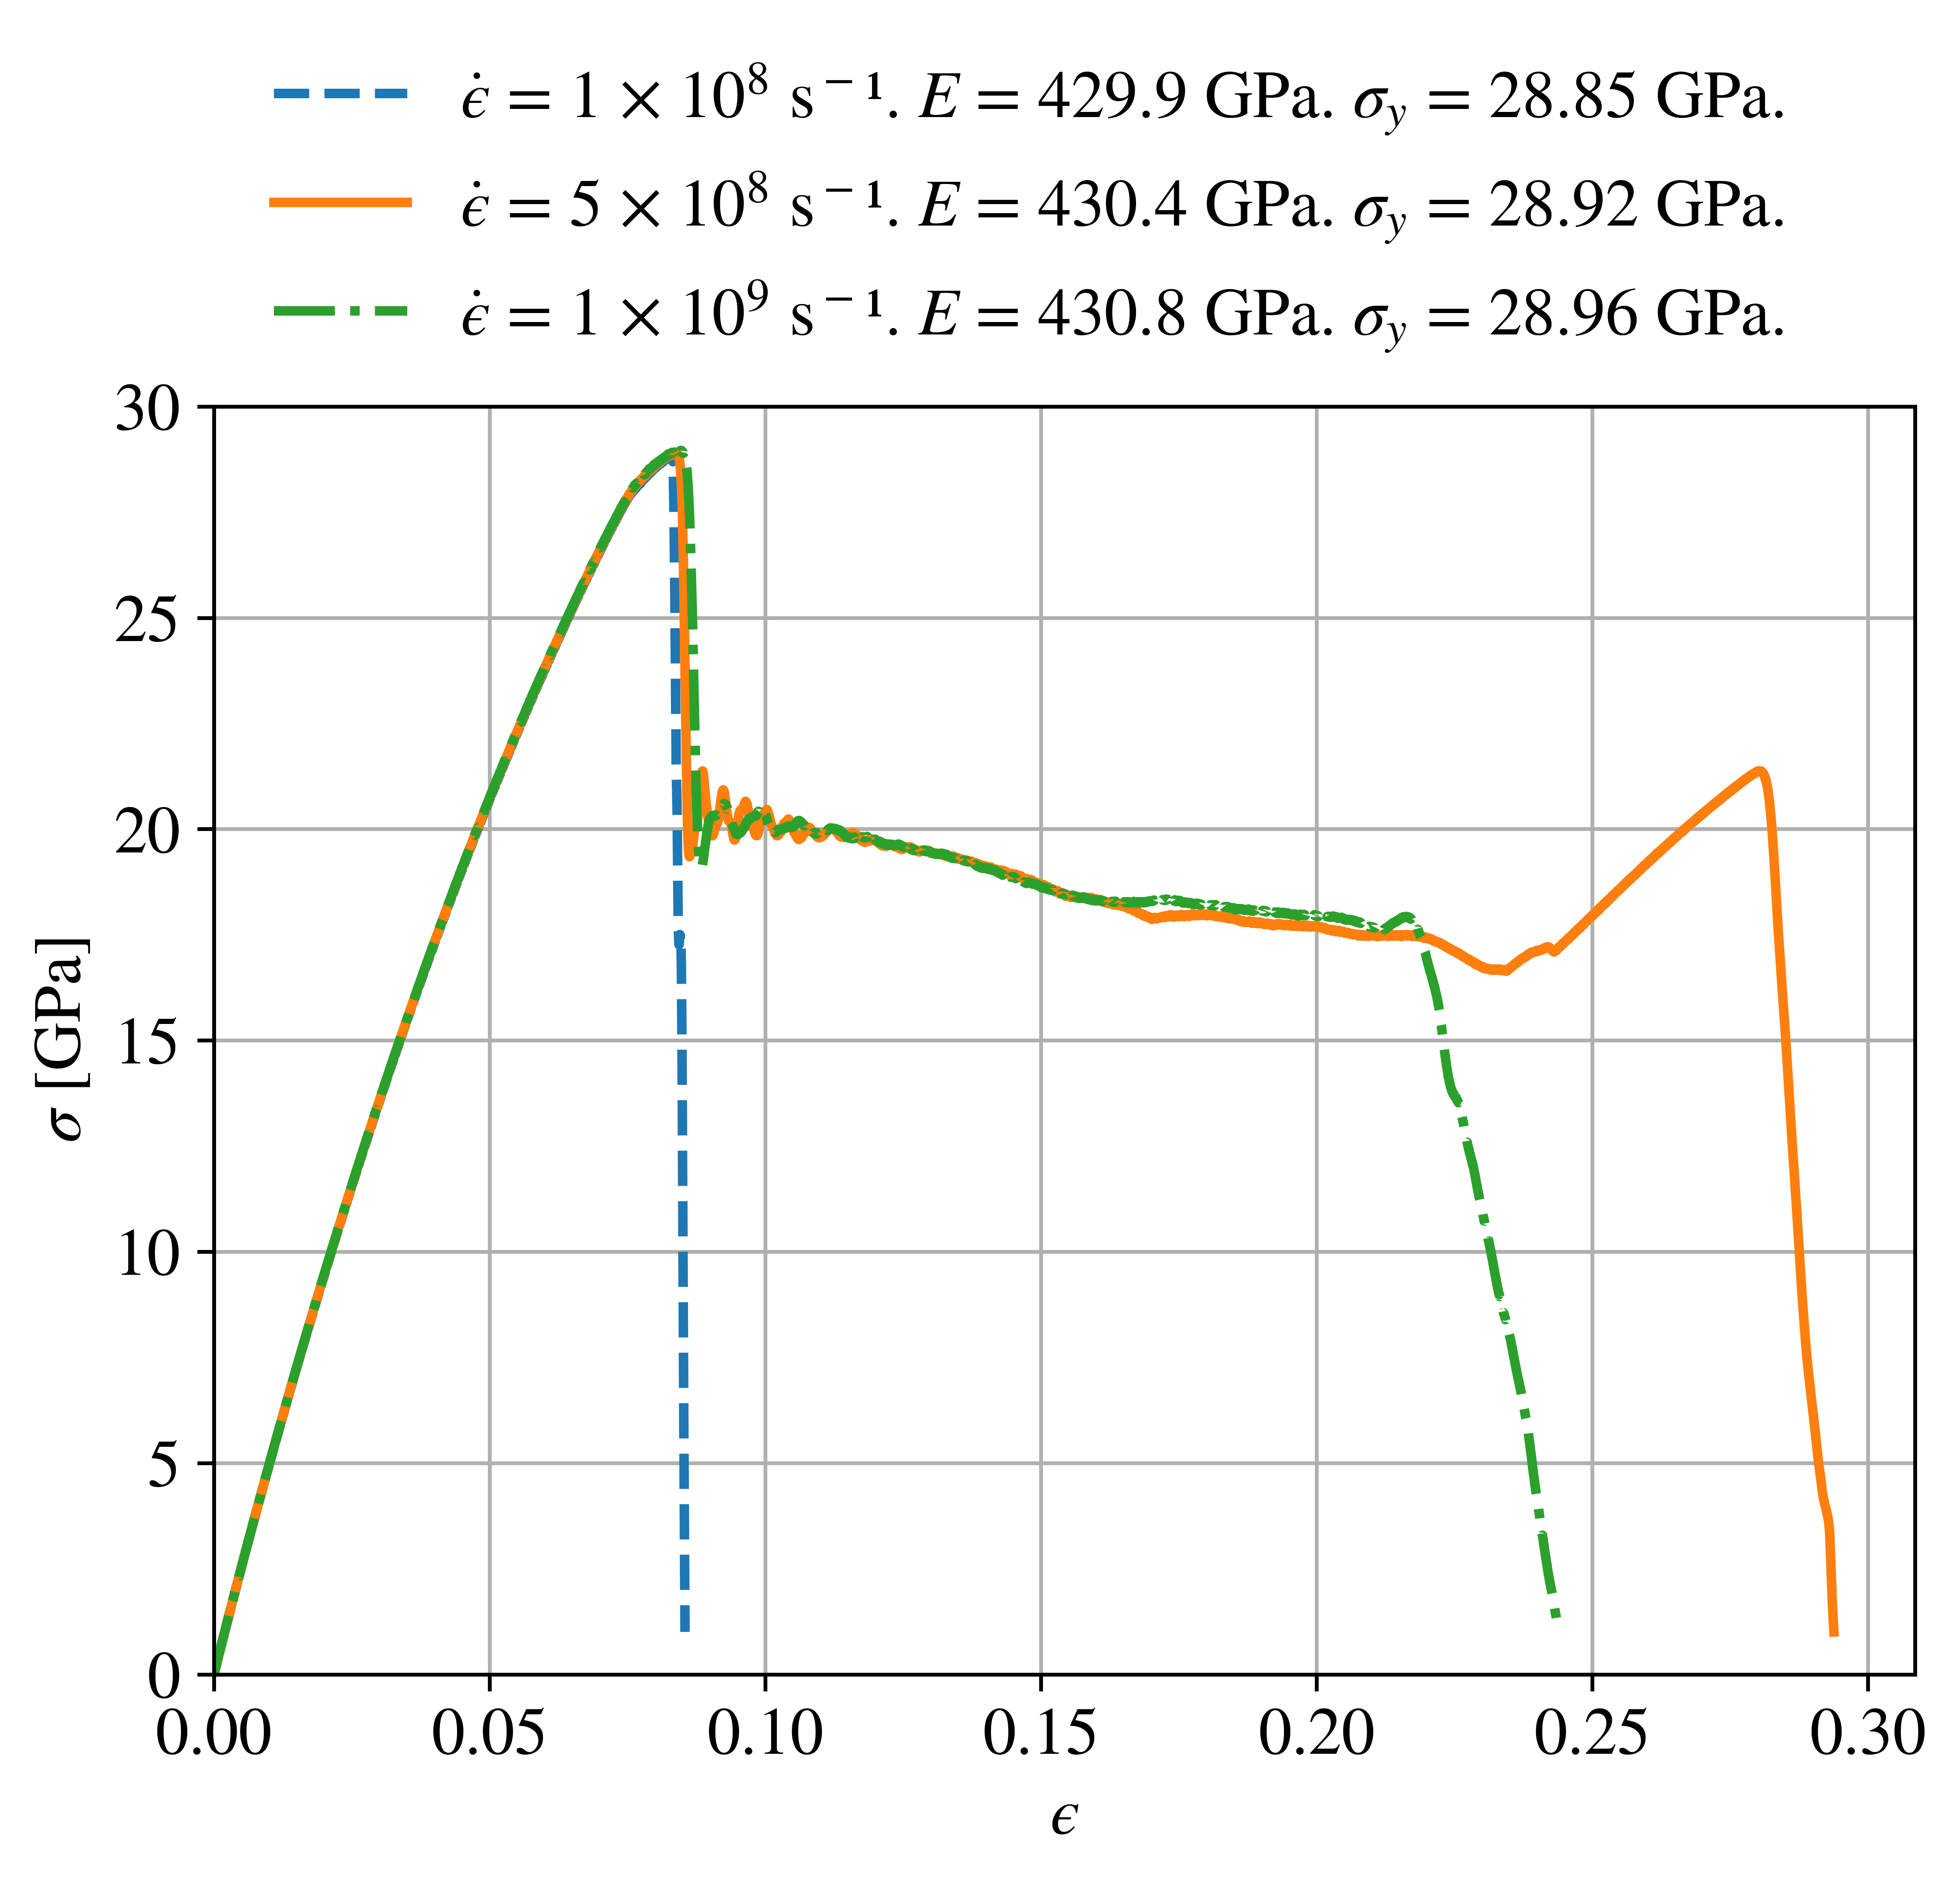
\includegraphics[width=0.48\textwidth]{SS-2-ADP.png} \label{Fig:SS-ADP-PBCs}}
\hfill
\subfloat[Kocevski potential + Full PBCs]{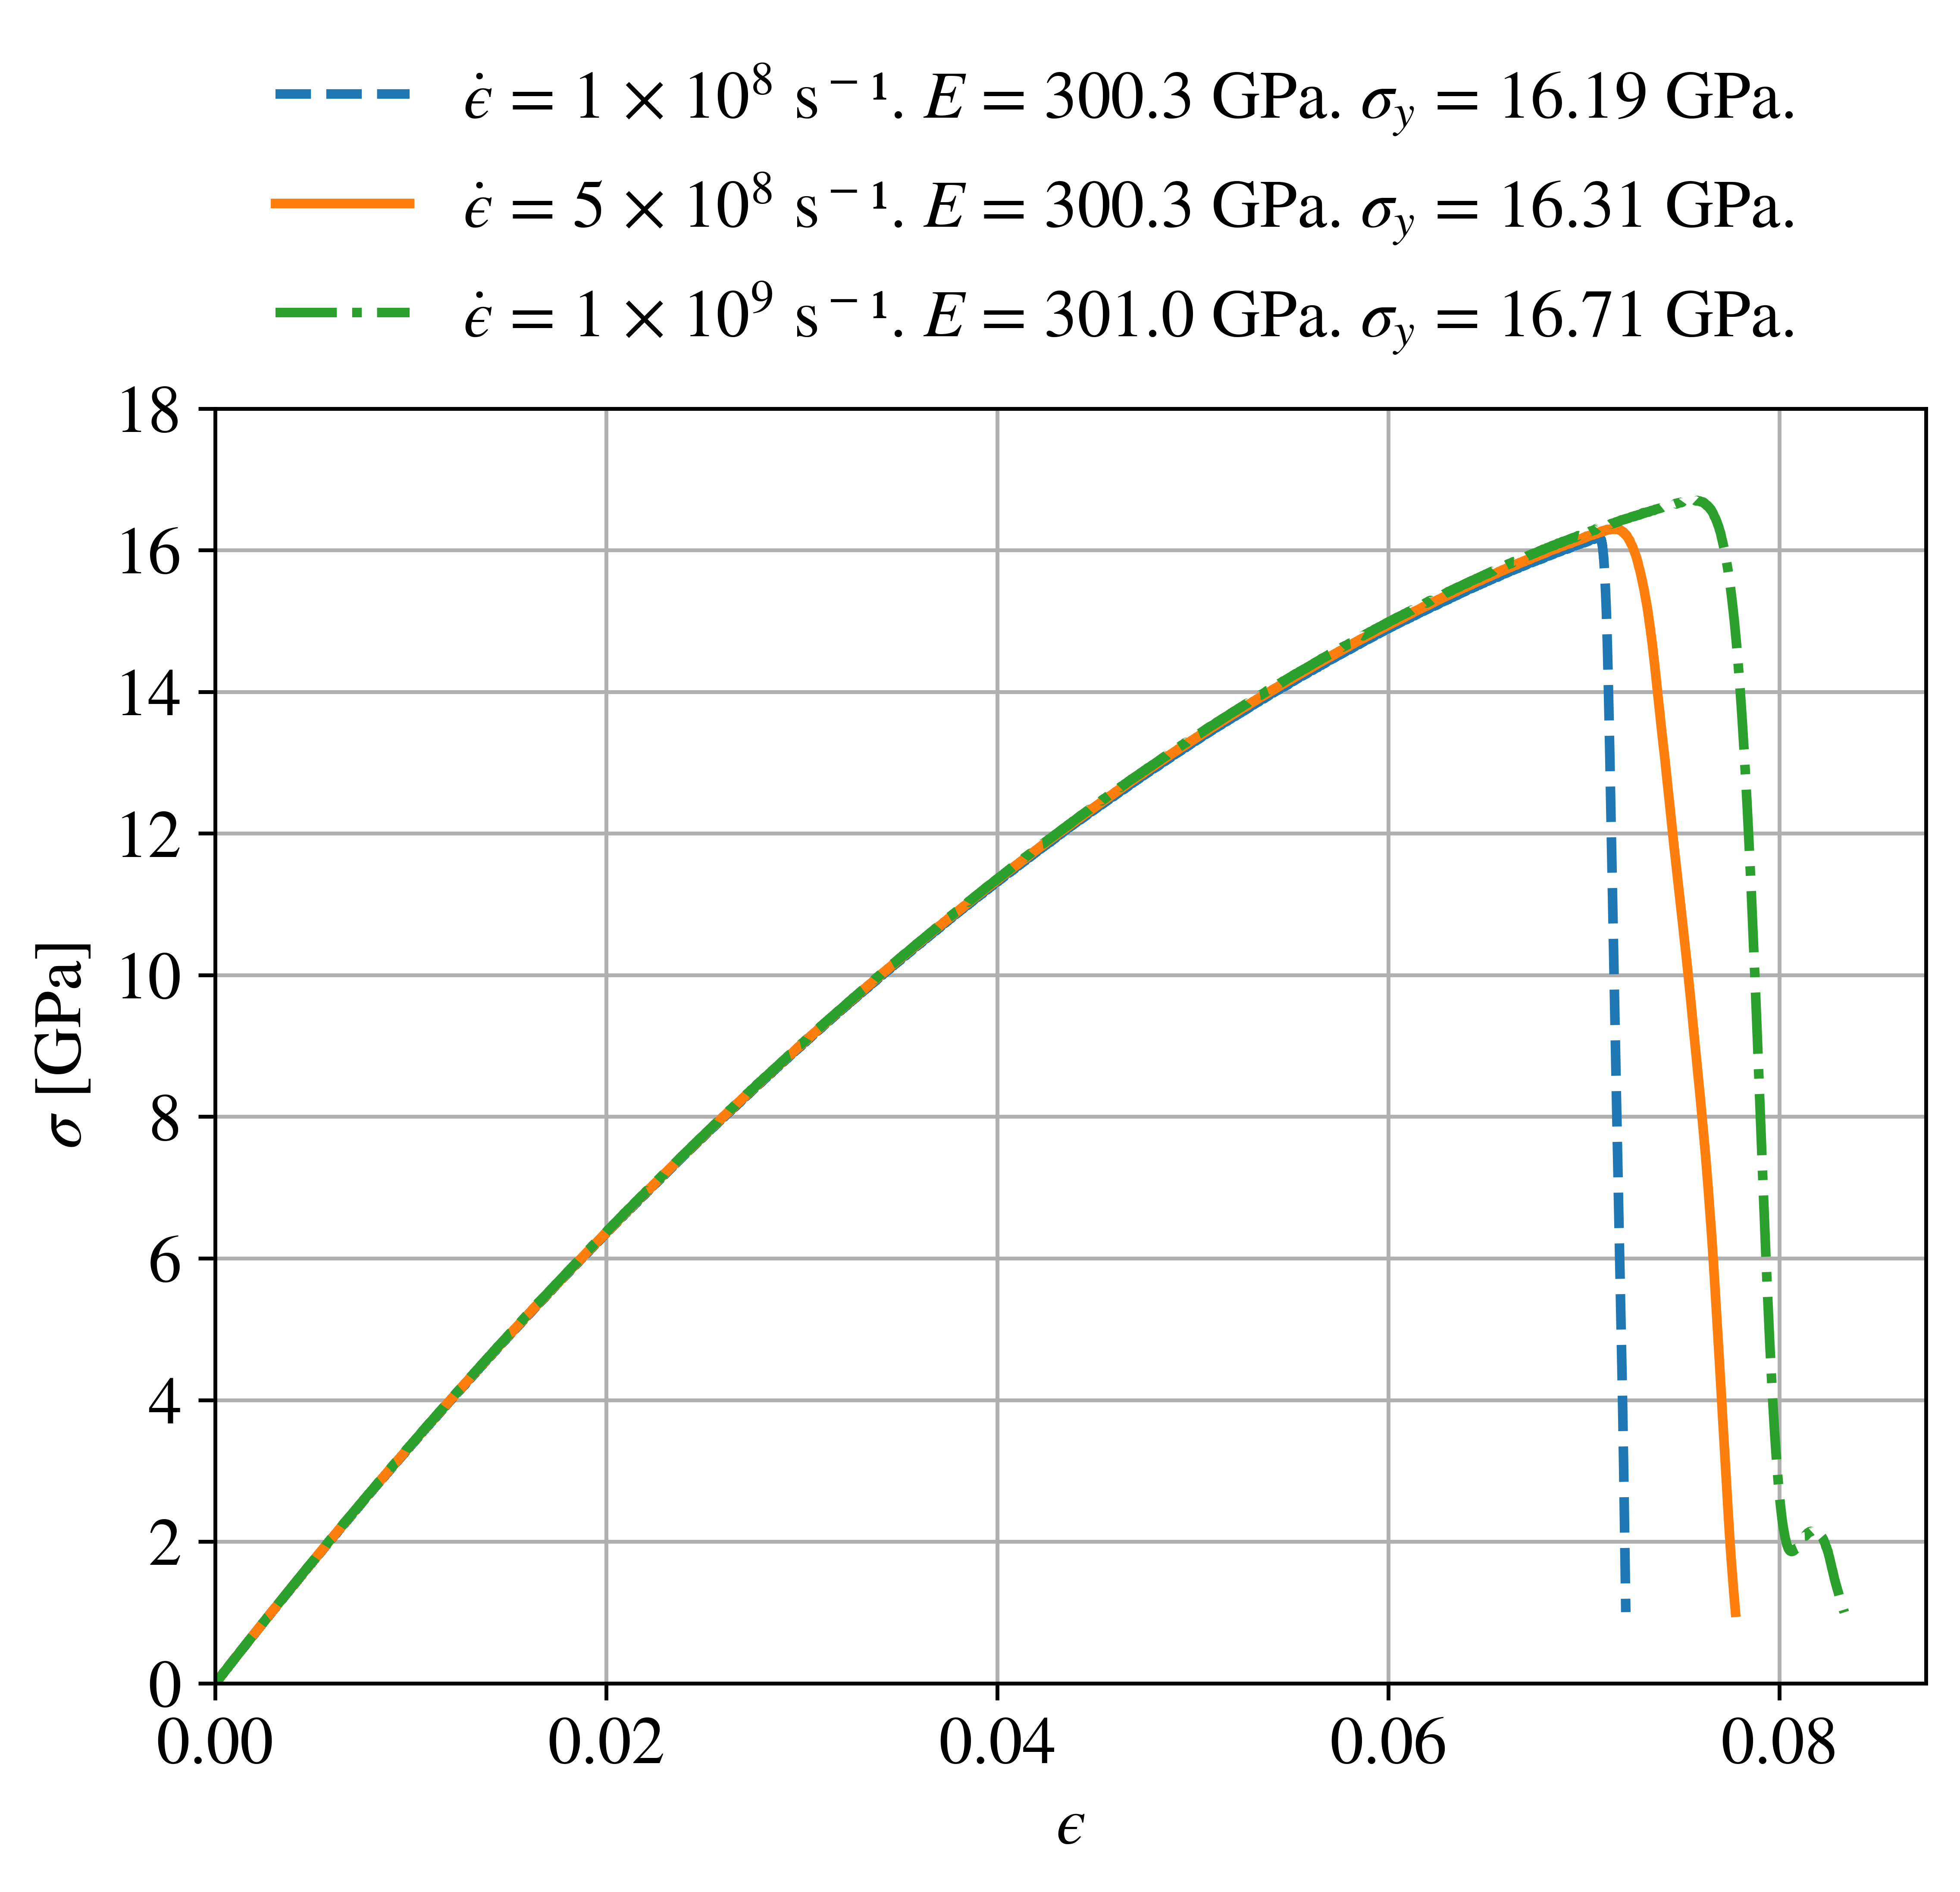
\includegraphics[width=0.48\textwidth]{SS-2-EAM.png} \label{Fig:SS-EAM-PBCs}}
\hfill
\subfloat[Tseplyaev potential + Free surfaces]{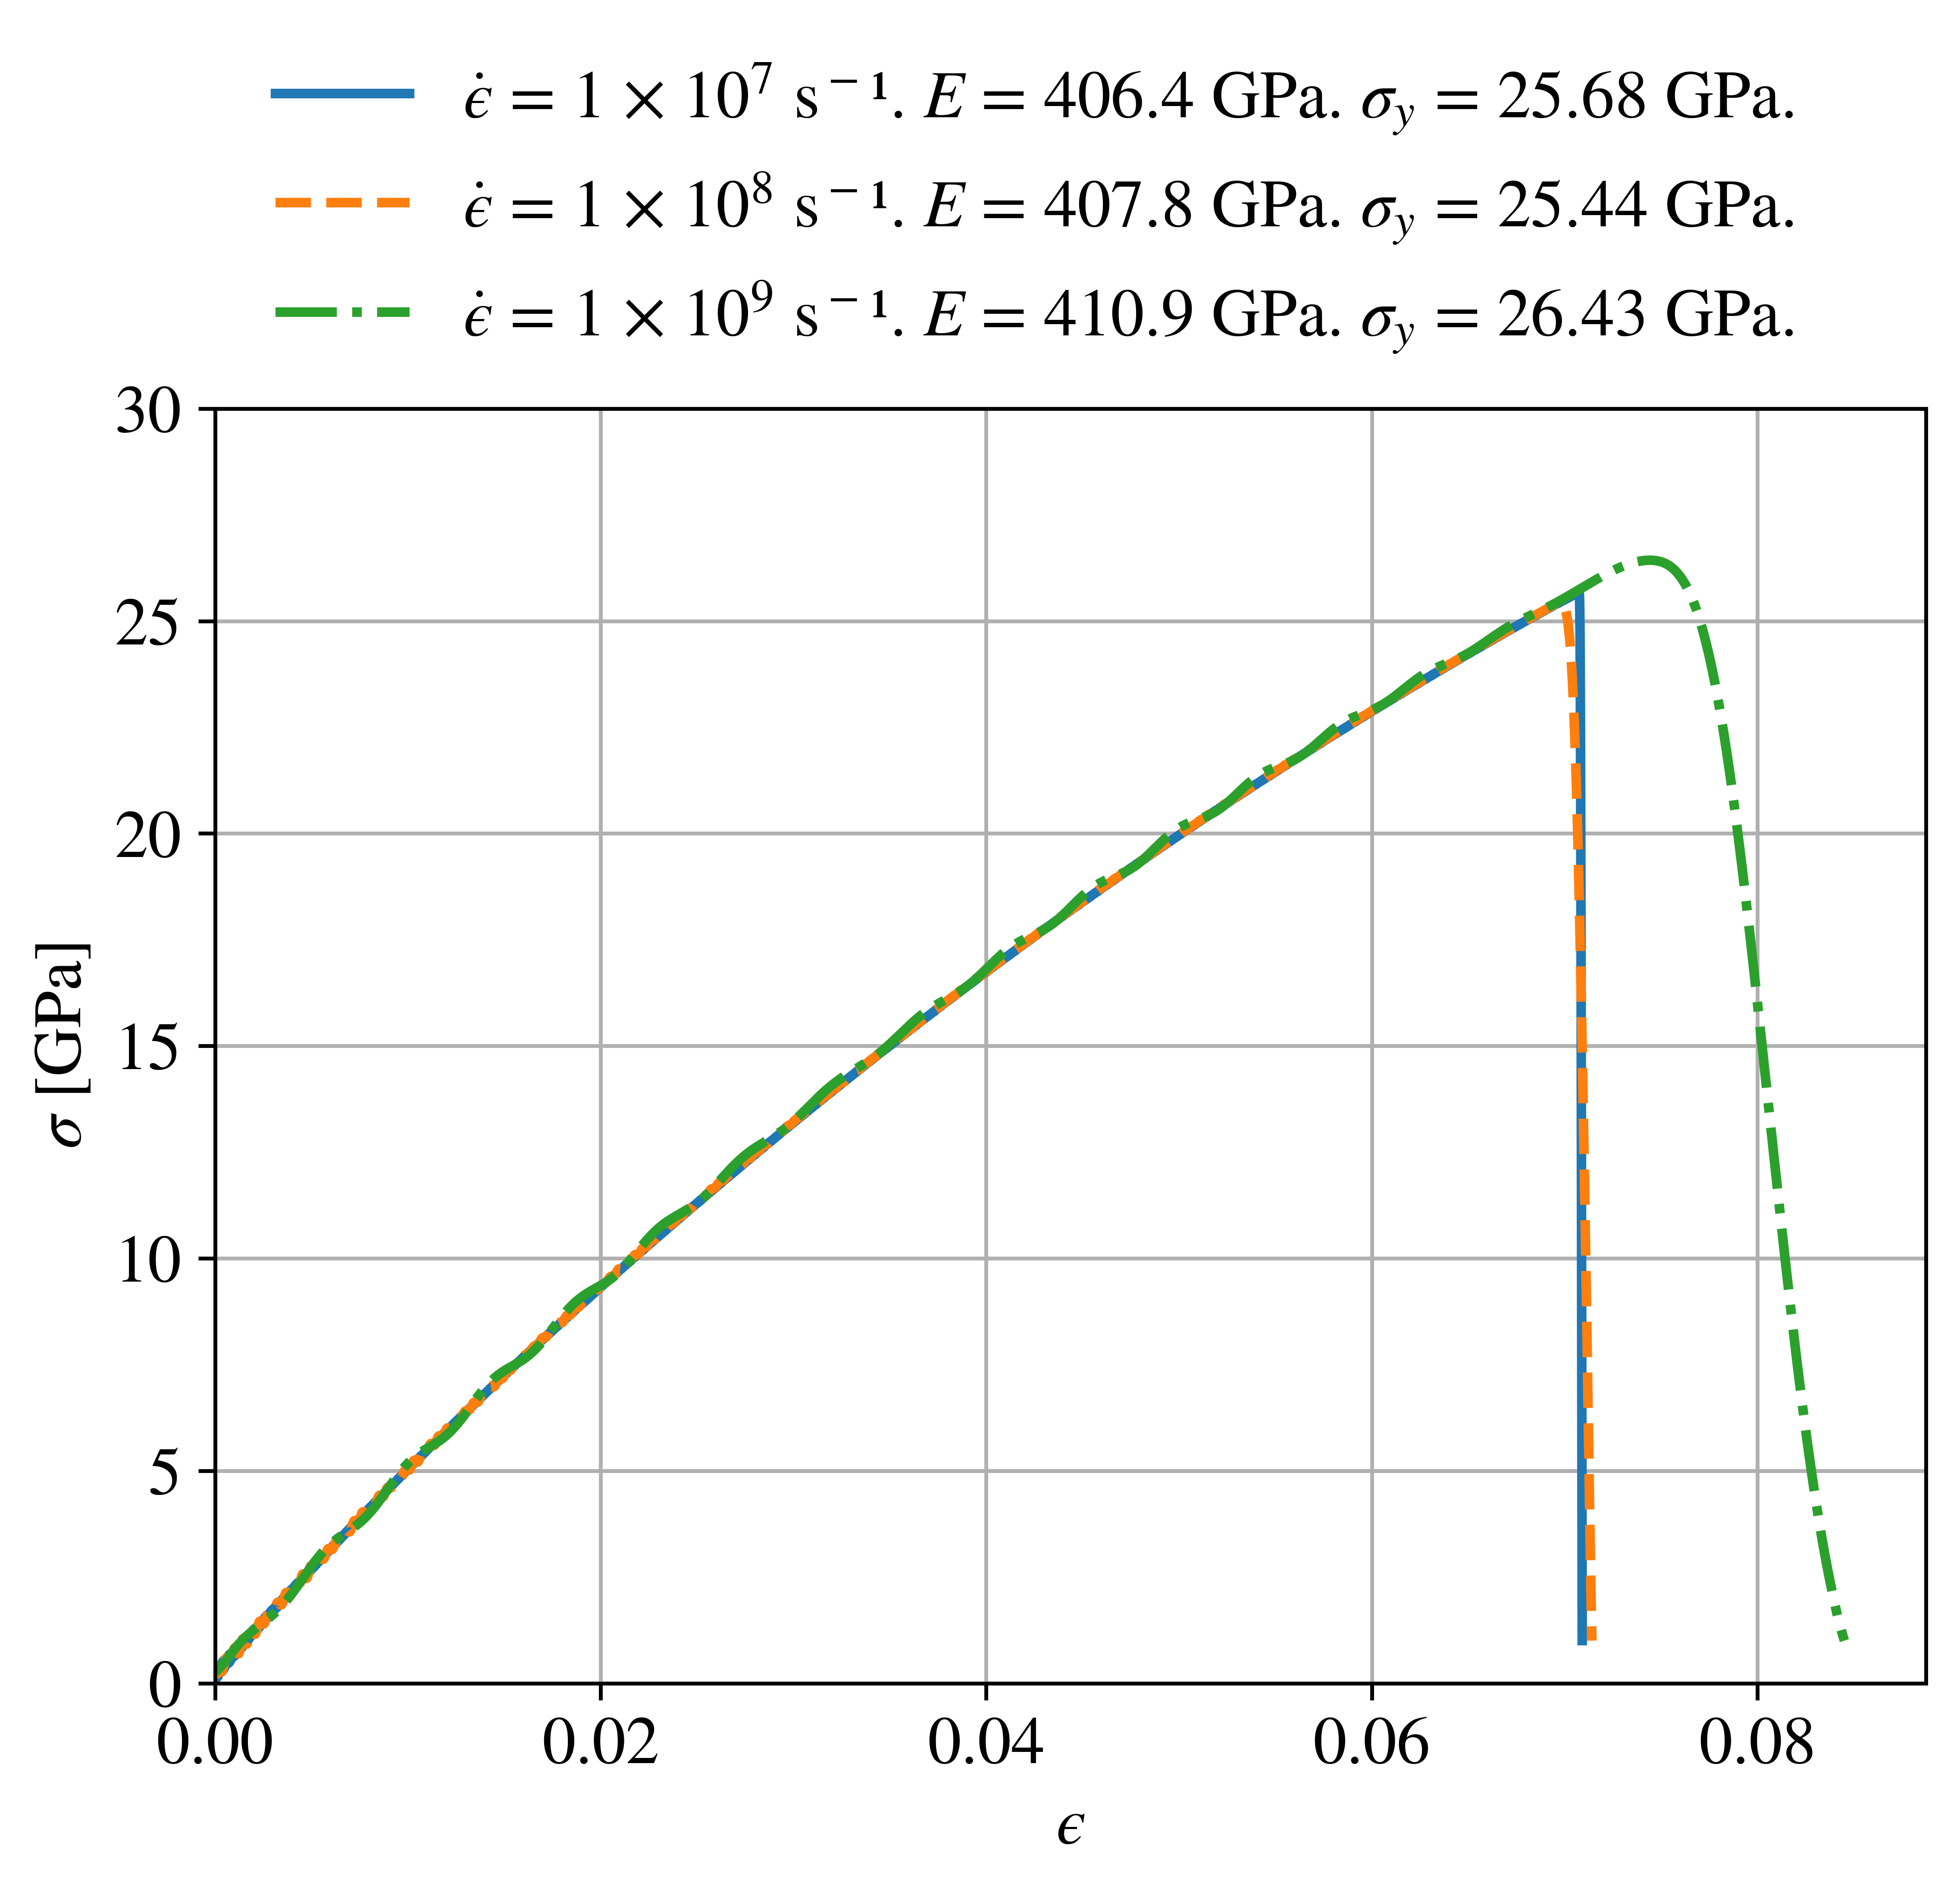
\includegraphics[width=0.48\textwidth]{SS-1-ADP.png} \label{Fig:SS-ADP-FreeSurf}}    
\hfill
\subfloat[Kocevski potential + Free surfaces]{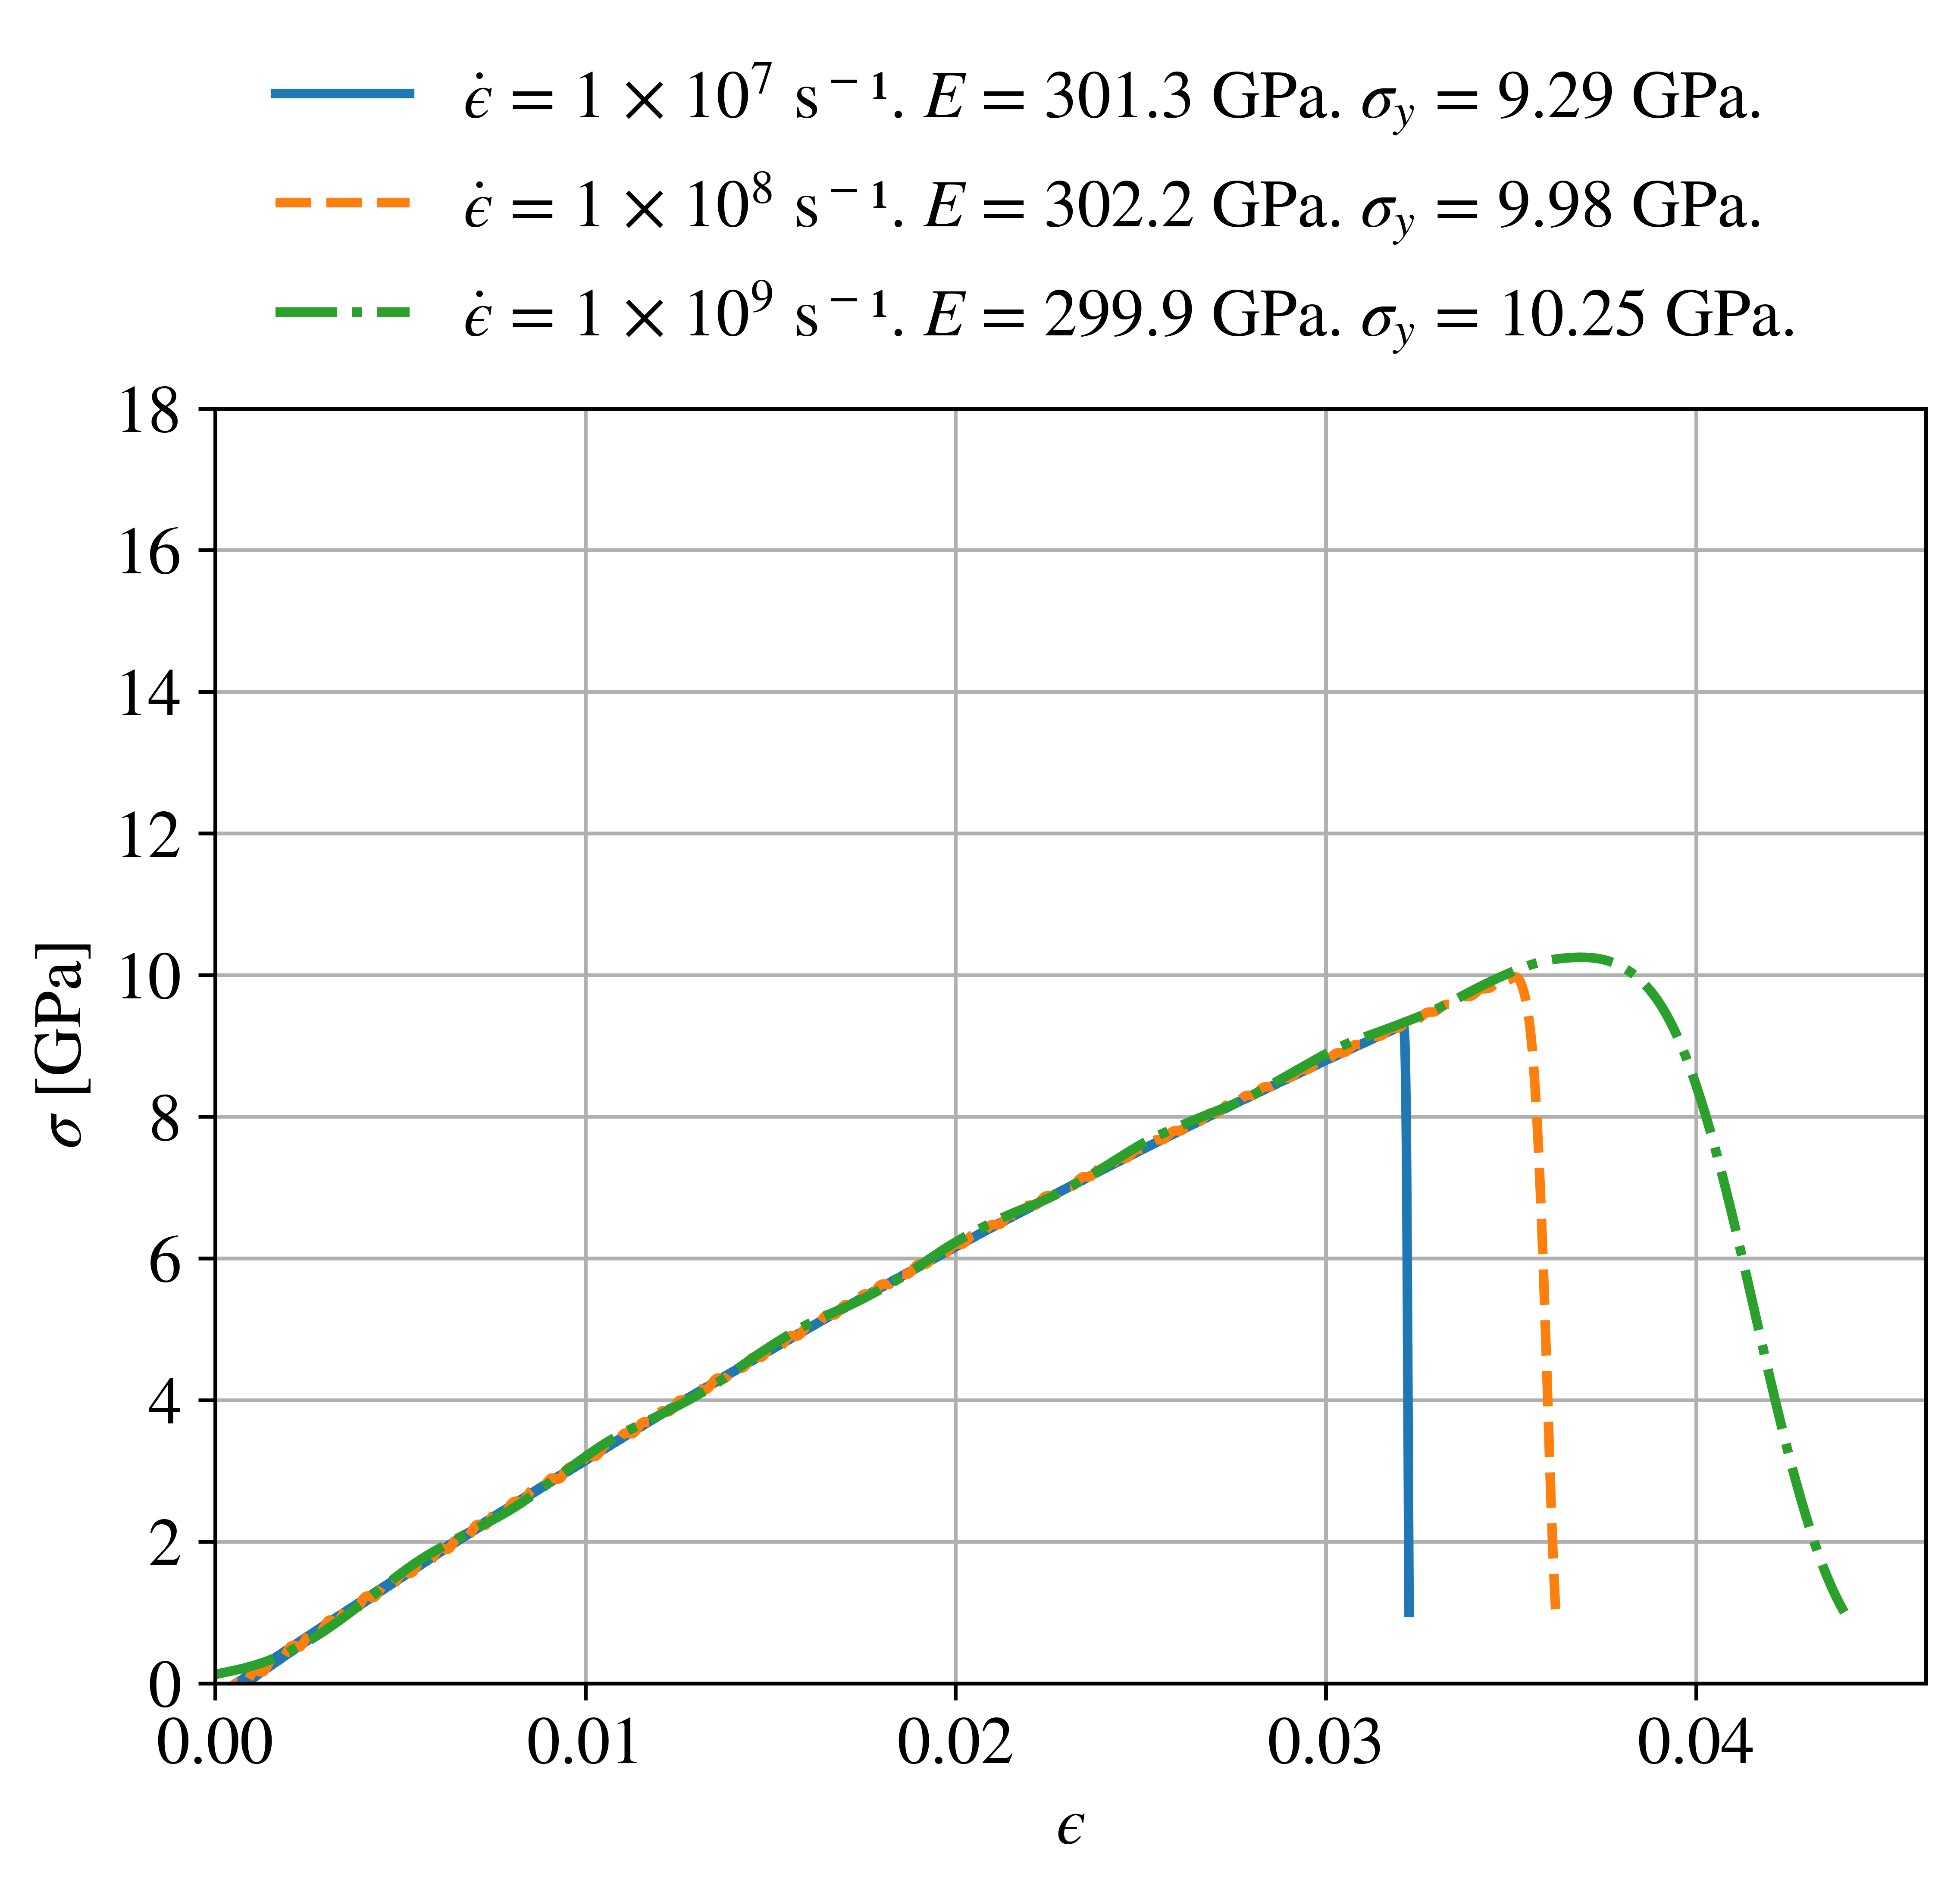
\includegraphics[width=0.48\textwidth]{SS-1-EAM.png} \label{Fig:SS-EAM-FreeSurf}}

\caption{(Color online) Stress-strain curves of UN computed at 300 K by \textbf{(a)} the Tseplyaev potential and \textbf{(b)} the Kocevski potential under different strain rates with PBCs applied in all directions. Stress-strain curves of UN computed at 300 K by \textbf{(c)} the Tseplyaev potential and \textbf{(d)} the Kocevski potential under different strain rates with PBCs applied only along the loading direction. To suppress the effect of pressure oscillations on the stress-strain curves for supercells with free surfaces, the curves calculated by the Tseplyaev and Kocevski potentials have been smoothed by a moving average with a window of 2 and 4 ps, respectively. Note that the $y$-axis range is the same for each potential whereas the $x$-axis is unique for each figure.}
\label{Fig:SS}
\end{figure}

\begin{table}[h!]
\centering
\caption{Small-strain Young's modulus along the [100] direction, $E_{[100]}$ (\cref{Eq:E100}), as well as the nanoindentation hardness, $H$, of UN as predicted by both potentials and compared to experimental values at room temperature. The nanoindentation hardness value of Adachi \textit{et al.} \cite{Adachi2009} represents an average of measurements with loads $< 0.01$ N where the indentation size effect is not apparent.}
\footnotesize
\begin{tabular}{cccc} 
\hline
                    & Tseplyaev     & Kocevski  & Experimental \\
\hline
$E_{[100]}$ [GPa]   & 522.7         & 354.1     & 387.0 \cite{Salleh1986}   \\
$H$ [GPa]           & 25.38         & 9.28      & 7.8 $\pm$ 0.2 \cite{Frazer2021}, 9.7 $\pm$ 0.4 \cite{Adachi2009}    \\
\hline
\end{tabular}
\label{Tab:E100}
\end{table}

% The velocity of the deformation can be estimated from:
% \begin{equation}
% v = \Dot{\epsilon} l_x
% \end{equation}
% where $l_x$ is the dimension of the supercell along the loading/tensile direction.

The yield stresses predicted by the Tseplyaev potential for nanocrystalline UN strained under PBCs (\cref{Fig:SS-ADP-PBCs}) are larger than that predicted by the Kocevski potential (\cref{Fig:SS-EAM-PBCs}) by more than a factor of 2. Ultrahigh yield stresses in the range of about 30 GPa predicted by the Tseplyaev potential are characteristic of purely covalent nanomaterials like Si and SiC \cite{Ivashchenko2007}, which is not the case for UN whose bonding environment has both ionic and covalent character \cite{Kuksin2016}. At all strain rates, the Kocevski potential predicts brittle fracture for nanocrystalline UN (\cref{Fig:SS-EAM-PBCs}). Interestingly, however, for strain rates of $5 \times 10^{8}$ and $10^{9}$ s$^{-1}$, the Tseplyaev potential predicts sustainable plastic deformation by dislocation motion along the $\{ 111 \}$ planes (\cref{Fig:Slip}). The stress-strain curves show signs of stress relaxation after yielding and multiple slip planes develop along the entire length of the specimen. The drop in the stress-strain curve after yielding is attributed to the development of dislocation planes \cite{Pal2020}. Necking occurs as a result of the branching of secondary dislocation planes from a primary dislocation plane \cite{Pal2020} as can be observed in \cref{Fig:Slip}.

\begin{figure}[h!]
    \centering
    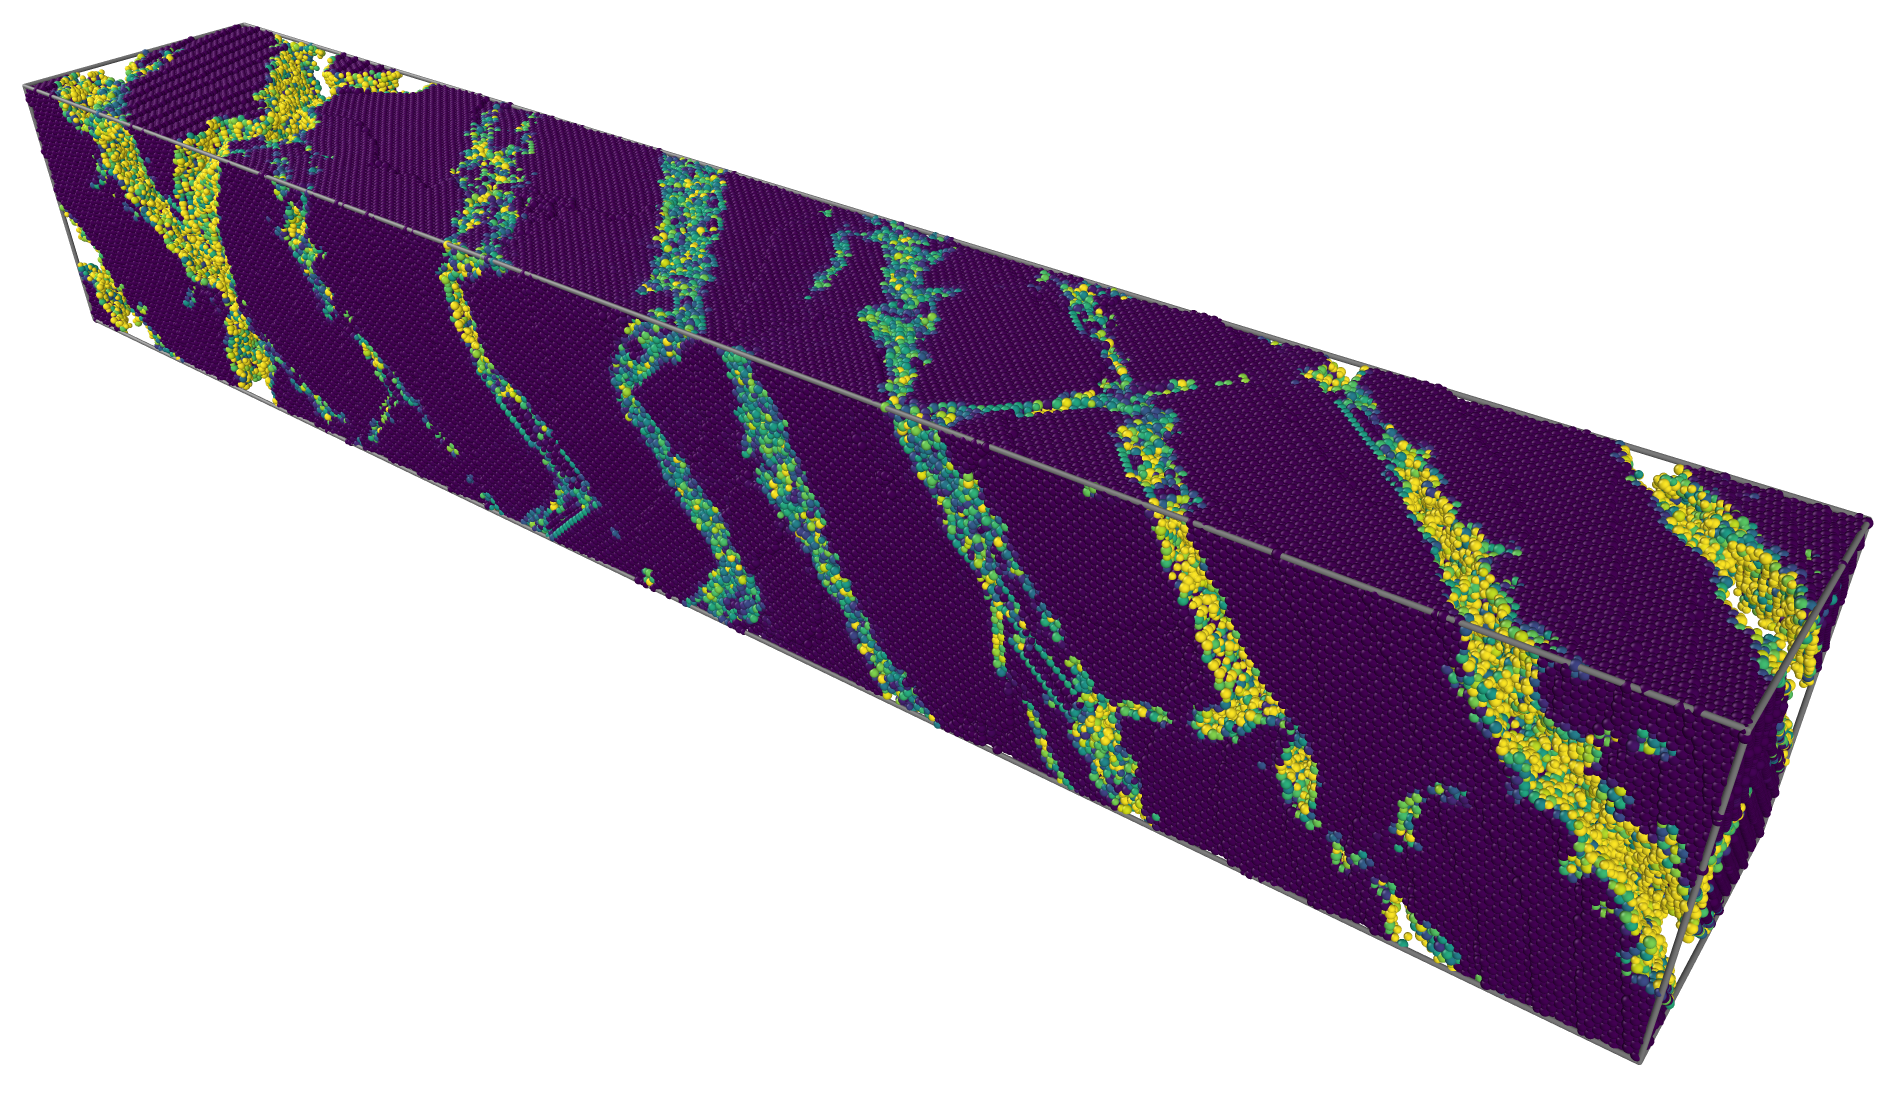
\includegraphics[width=0.70\textwidth]{SlipADP1e9.png}
    \caption{(Color online) $\{ 111 \}$ slip planes generated in the $150 \times 30 \times 30$ supercell when strained at 300 K and a strain rate of $10^{9}$ s$^{-1}$ under PBCs as modeled by the Tseplyaev potential. Atoms have been colored in OVITO according to their CSP where dark purple atoms have zero CSP and yellow atoms have high CSP. For better visibility, the maximum CSP has been set to 20 \AA$^2$. Similar slip planes have been observed at a strain rate of $5 \times 10^{8}$ s$^{-1}$.}
    \label{Fig:Slip}
\end{figure}

The finding that UN slips primarily along the $\{111\}$ planes is interesting because it contradicts the principal slip system reported by Sole and van der Walt for UN, which is $\{110\}$ \cite{Sole1968}. $\{110\}$ planes are the preferred slip system for purely ionic crystals \cite{VanDerWalt1967, Hull2011}. For crystals with a mixed ionic-covalent bonding environment (as in the case of UN), slip might principally occur along other planes, e.g., $\{111\}$ and $\{100\}$ \cite{VanDerWalt1967, Yadav2014}. More interestingly, the primary slip planes in UC and TiC, two compounds closely related to UN, have been reported to be $\{111\}$ \cite{Sole1968, Vasudevamurthy2022}, which raises questions about the physical reason for this discrepancy.

Van der Walt and Sole attempted to explain the different slip systems of UN and UC in another study \cite{VanDerWalt1967} by formulating a hard sphere model for MX compounds with the NaCl crystal structure in which the radius ratio, i.e., $R_\text{X}/R_\text{M}$, affects the saddle point configuration of the $\frac{1}{2}\langle110\rangle$ dislocation during its motion. Based on this model, three cases arise: (\textit{a}) crystals with $R_\text{X}/R_\text{M} \approx 0.414$ slip on $\{110\}$; (\textit{b}) for $0.414 < R_\text{X}/R_\text{M} < 0.633$, slip is on $\{111\}$; and (\textit{c}) for $R_\text{X}/R_\text{M} > 0.633$, slip occurs on $\{100\}$. They further assumed that $R_\text{M}$ equals the metallic radius, and $R_\text{X} = a_\text{MX}/2 - R_\text{M}$, where $a_\text{MX}$ is the lattice parameter of the compound MX. Based on this definition, the authors found that for UN, $R_\text{X}/R_\text{M} = 0.41$ which predicts slip on $\{110\}$, whereas for UC, $R_\text{X}/R_\text{M} = 0.43$ which predicts slip on $\{111\}$. However, the choice of the metallic radius, $R_\text{M}$, is rather arbitrary.

To confirm that we are observing dislocations along slip planes, the DXA algorithm was applied to the supercell immediately after fracture, and it was found that perfect dislocations (of both edge and screw characters) with $\mathbf{b} = \frac{1}{2} \langle 110 \rangle$ (which is the usual Burgers vector in ionic crystals \cite{Hull2011}) reside along the planes with a high CSP. We also found many Shockley partials with a Burgers vector $\frac{1}{6}\langle112\rangle$ along the same planes. Historically, the existence of Shockley partials in ionic crystals has been the source of much debate in the literature \cite{Smoluchowski1966, Haasen1985}. Based on geometrical and energetic arguments, it was shown that for an ionic MX compound that has the NaCl crystal structure and slips on the $\{111\}$ planes, only perfect dislocations can exist because the presence of the smaller X atoms prevents the occurrence of Shockley partials \cite{VanDerWalt1967}. Thus, the observed Shockley partials may be either an artifact of the dislocation analysis algorithm or an intermediate metastable state predicted by the Tseplyaev potential. Another possibility is that the Tspelyaev potential overestimates the covalency of UN. In \cref{Fig:Slip}, we can also see signs of cross-slip along planes of the $\{111\}$ family. This is expected, as cross slip of screw dislocations with $\mathbf{b} = \frac{1}{2}\langle110\rangle$ can occur only by glide on planes other than $\{110\}$, as only one $\langle110\rangle$ direction lies in a given $\{110\}$ plane \cite{Hull2011}.

It should be pointed out that at a strain rate of $10^{8}$ s$^{-1}$, the Tseplyaev potential shows no sign of dislocation formation or slip. The reason for this is that the formation of dislocations in a defect-free structure requires high energy deposition rates to form and move dislocations of large Burgers vectors \cite{Desai2008, Pal2020} which is only attainable at high strain rates. It should be emphasized that no dislocation nucleation is observed for the Kocevski potential, regardless of strain rate.

As expected, supercells with free surfaces (\cref{Fig:SS-ADP-FreeSurf,Fig:SS-EAM-FreeSurf}) show no signs of plastic behavior \cite{Ivashchenko2007}. Based on these curves, we have calculated estimates of the nanoindentation hardness that are outlined in \cref{Tab:E100}. To get these values, the maximum stresses of the stress-strain curves for supercells with free surfaces strained at rates of $10^7$, $10^8$, and $10^9$ s$^{-1}$ have been linearly extrapolated to a zero strain rate. It can be seen that the nanoindentation hardness estimated by the Kocevski potential is very close to the experimental value calculated by Frazer \textit{et al.} \cite{Frazer2021} at 300 K, whereas that estimated by the Tspelyaev potential is overestimated by more than a factor of 3. It should be emphasized that this method is based on an observed empirical correlation between the yield stress of the supercell with free surfaces and the nanoindentation hardness despite the deformation mechanisms in both being different. That is, nanoindentation experiments are associated with the formation of a plastic zone (with many dislocations) below the indent \cite{Adachi2009}, whereas the brittle fracture of the supercells with free surfaces shows no signs of plasticity. This correlation is justified because, although UN will fail through plastic deformation, its brittle fracture provides insight into the yield stress of the material \cite{Taylor2008} (which is often correlated with the hardness \cite{Meyers2009}), at which point the elastic limit is reached and plastic deformation initiates.

The nanoindentation hardness of UN couldn't be measured by Frazer \textit{et al.} \cite{Frazer2021} at $T > 473$ K due to the formation of an oxidation layer on the surfaces of UN samples at higher temperatures. In MD simulations, the formation of an oxidation layer is not an issue. Thus, this method can be used to estimate the nanoindentation hardness at higher temperatures provided we demonstrate that the empirical potential accurately predicts the mechanical behavior at the relevant temperatures.

\subsection{Dislocation motion}
\label{Sec:DislocMotion}

\subsubsection{Edge dislocations}

A schematic of the supercell constructed to study edge dislocations as well as OVITO visualization of the $\frac{1}{2} \langle 110 \rangle \{111\}$ edge dislocation and its Burgers vector after equilibration at 1 K are shown in \cref{Fig:DislocStructure}. It is noted that the Kocevski potential couldn't stabilize edge dislocations and only the Tseplyaev potential is used for their simulation. The gray ``defect mesh'' in \cref{Fig:DislocLine} extends over about two-thirds of $l_x$, as the dislocation's presence is not sensed far from the dislocation line. The defect mesh is an OVITO term for crystal regions where the atomic arrangement deviates from that of a perfect crystal. This implies that the chosen supercell dimensions are indeed large enough to have a strain-free state where PBCs are applied along the slip direction. A supercell similar to \cref{Fig:DislocStructure} was constructed for the screw dislocation, and the same observation about the defect mesh applies to it. We noted that after 0 K minimization, the $\frac{1}{2} \langle 110 \rangle \{111\}$ edge dislocation splits into two Shockley partials with $\mathbf{b} = \frac{1}{6} \langle 112 \rangle$. However, when the supercell is equilibrated at 1 K, the Shockley partials transform back to a perfect edge dislocation. Thus, the Tseplyaev potential predicts Shockley partials to exist only as a metastable state in UN. % Historically, there has been substantial debate on the existence of partial dislocations and stacking faults in ionic crystals \cite{Smoluchowski1966, Puls1976, Puls1980, Haasen1985}.

\begin{figure}[h!]
\centering
\subfloat[]{\label{Fig:Edge110}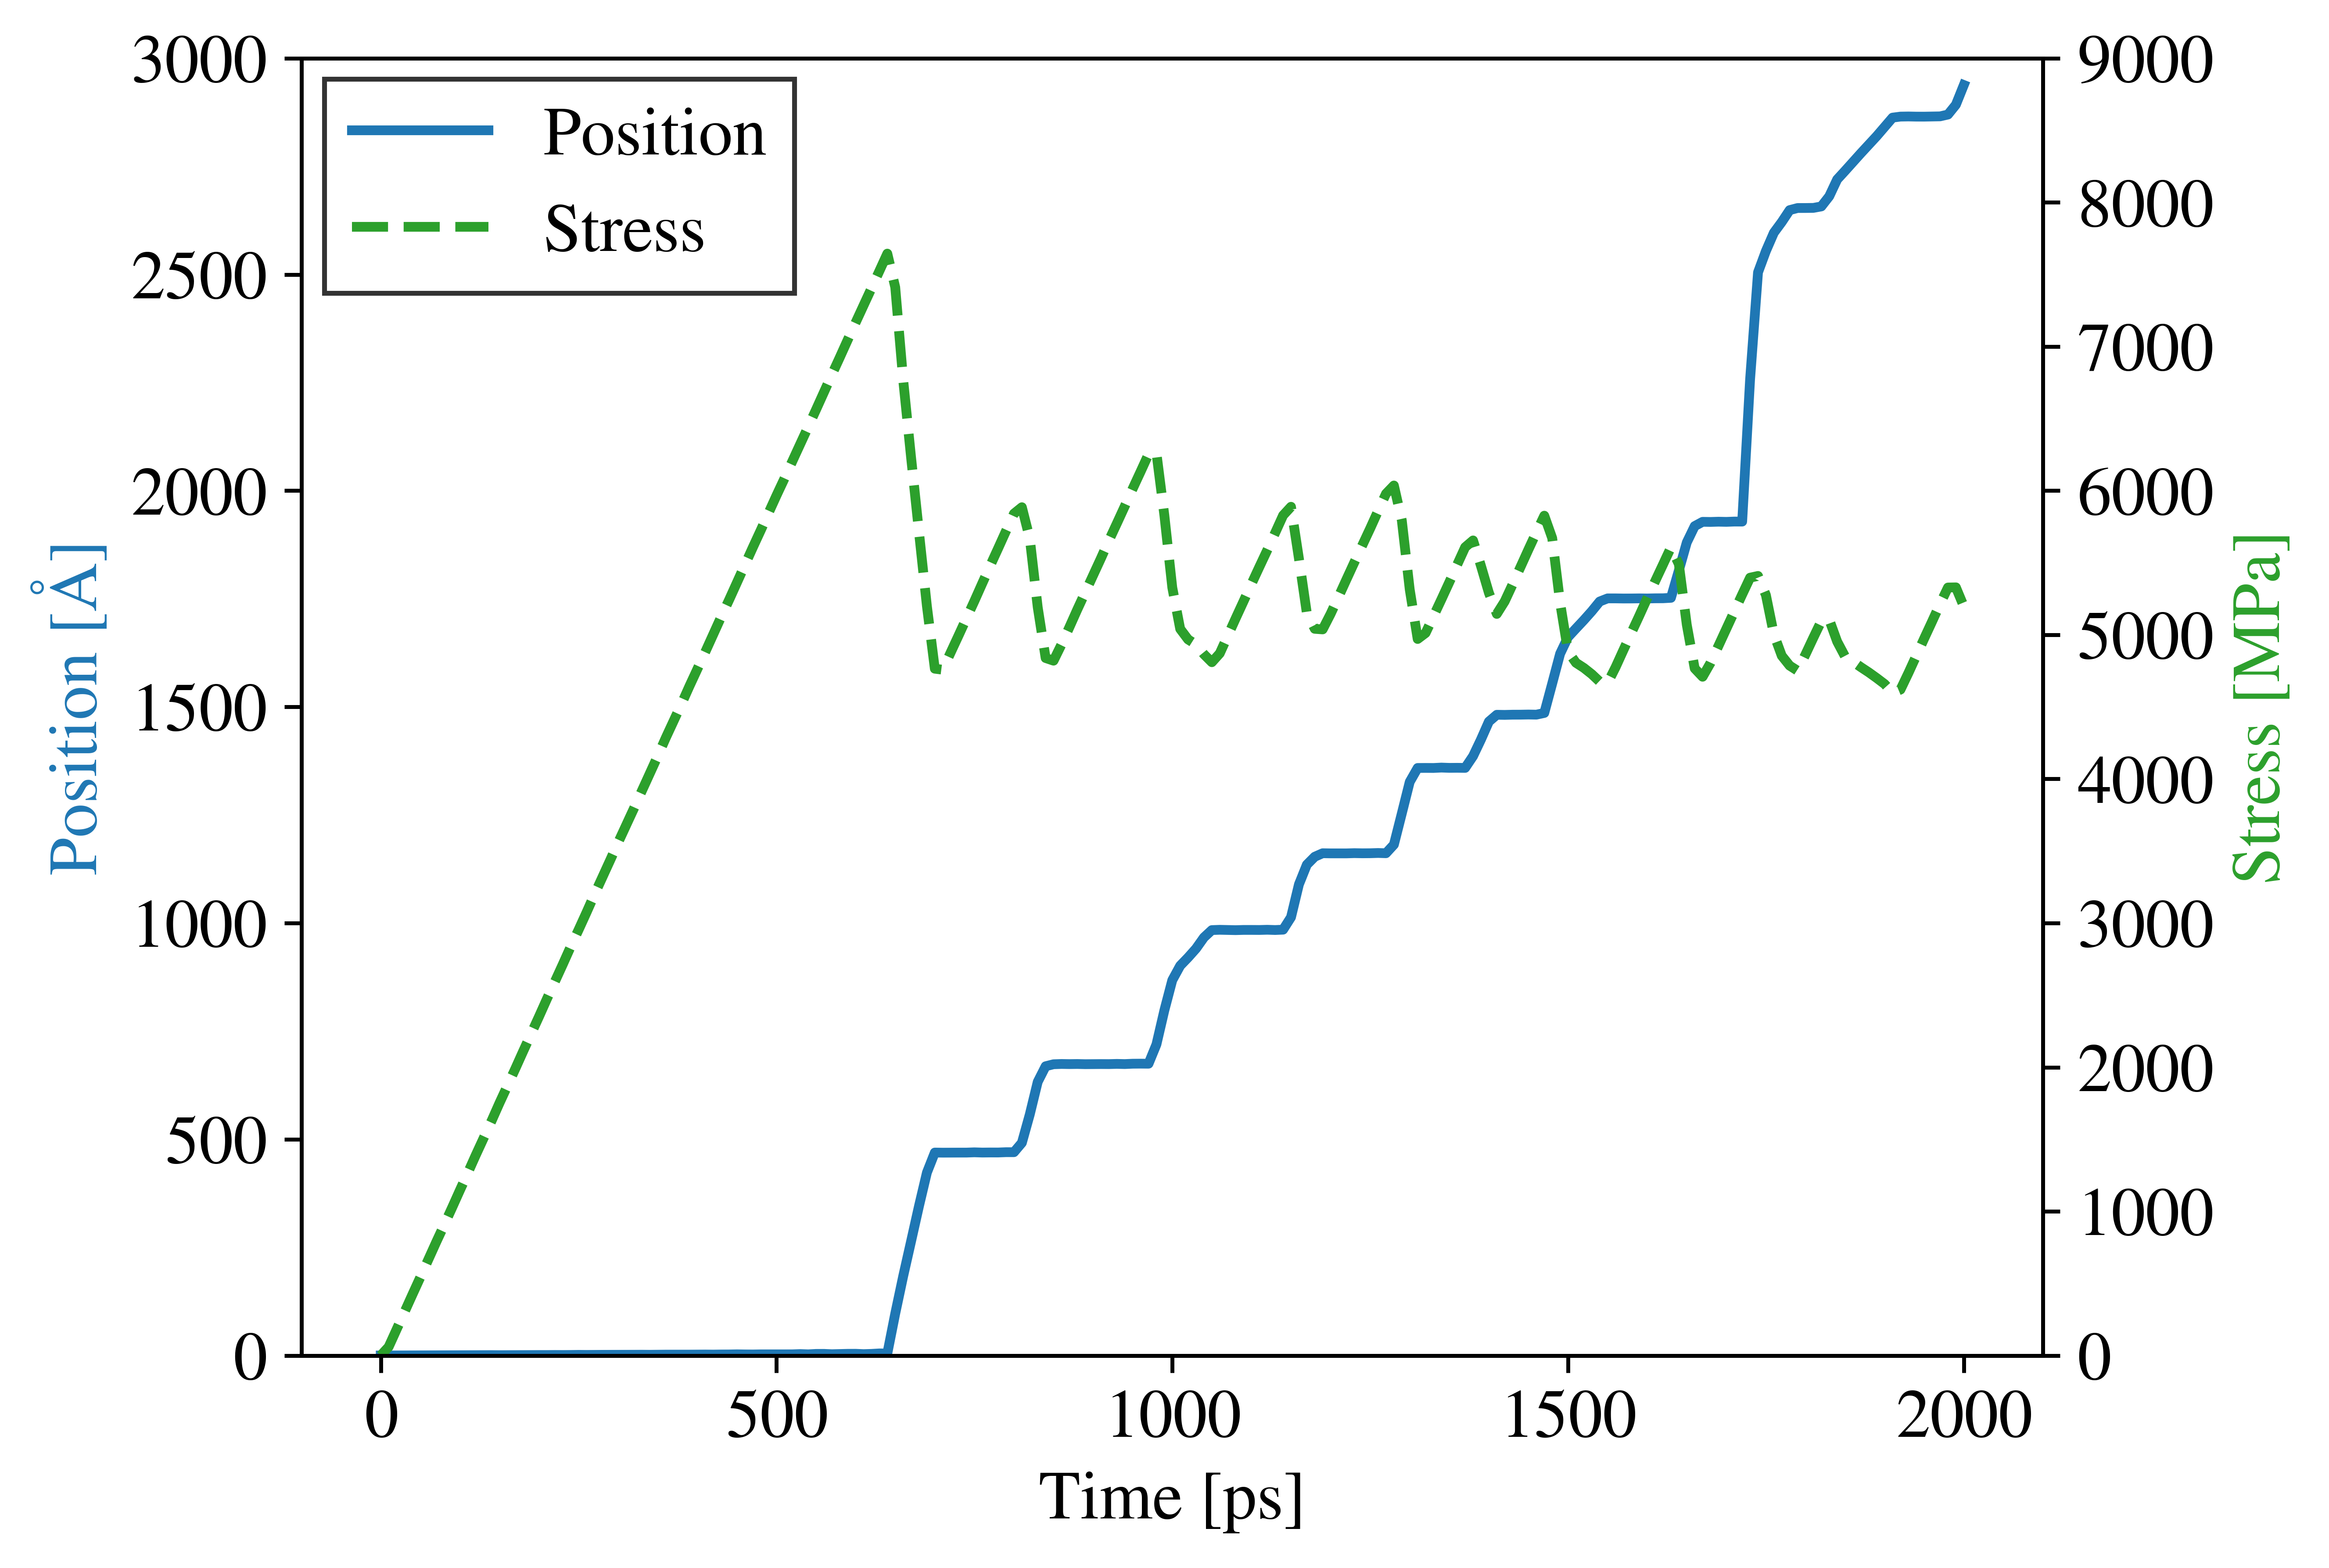
\includegraphics[width=0.48\textwidth]{Position-Stress-Edge110.png}}
\hfill
\subfloat[]{\label{Fig:Edge111}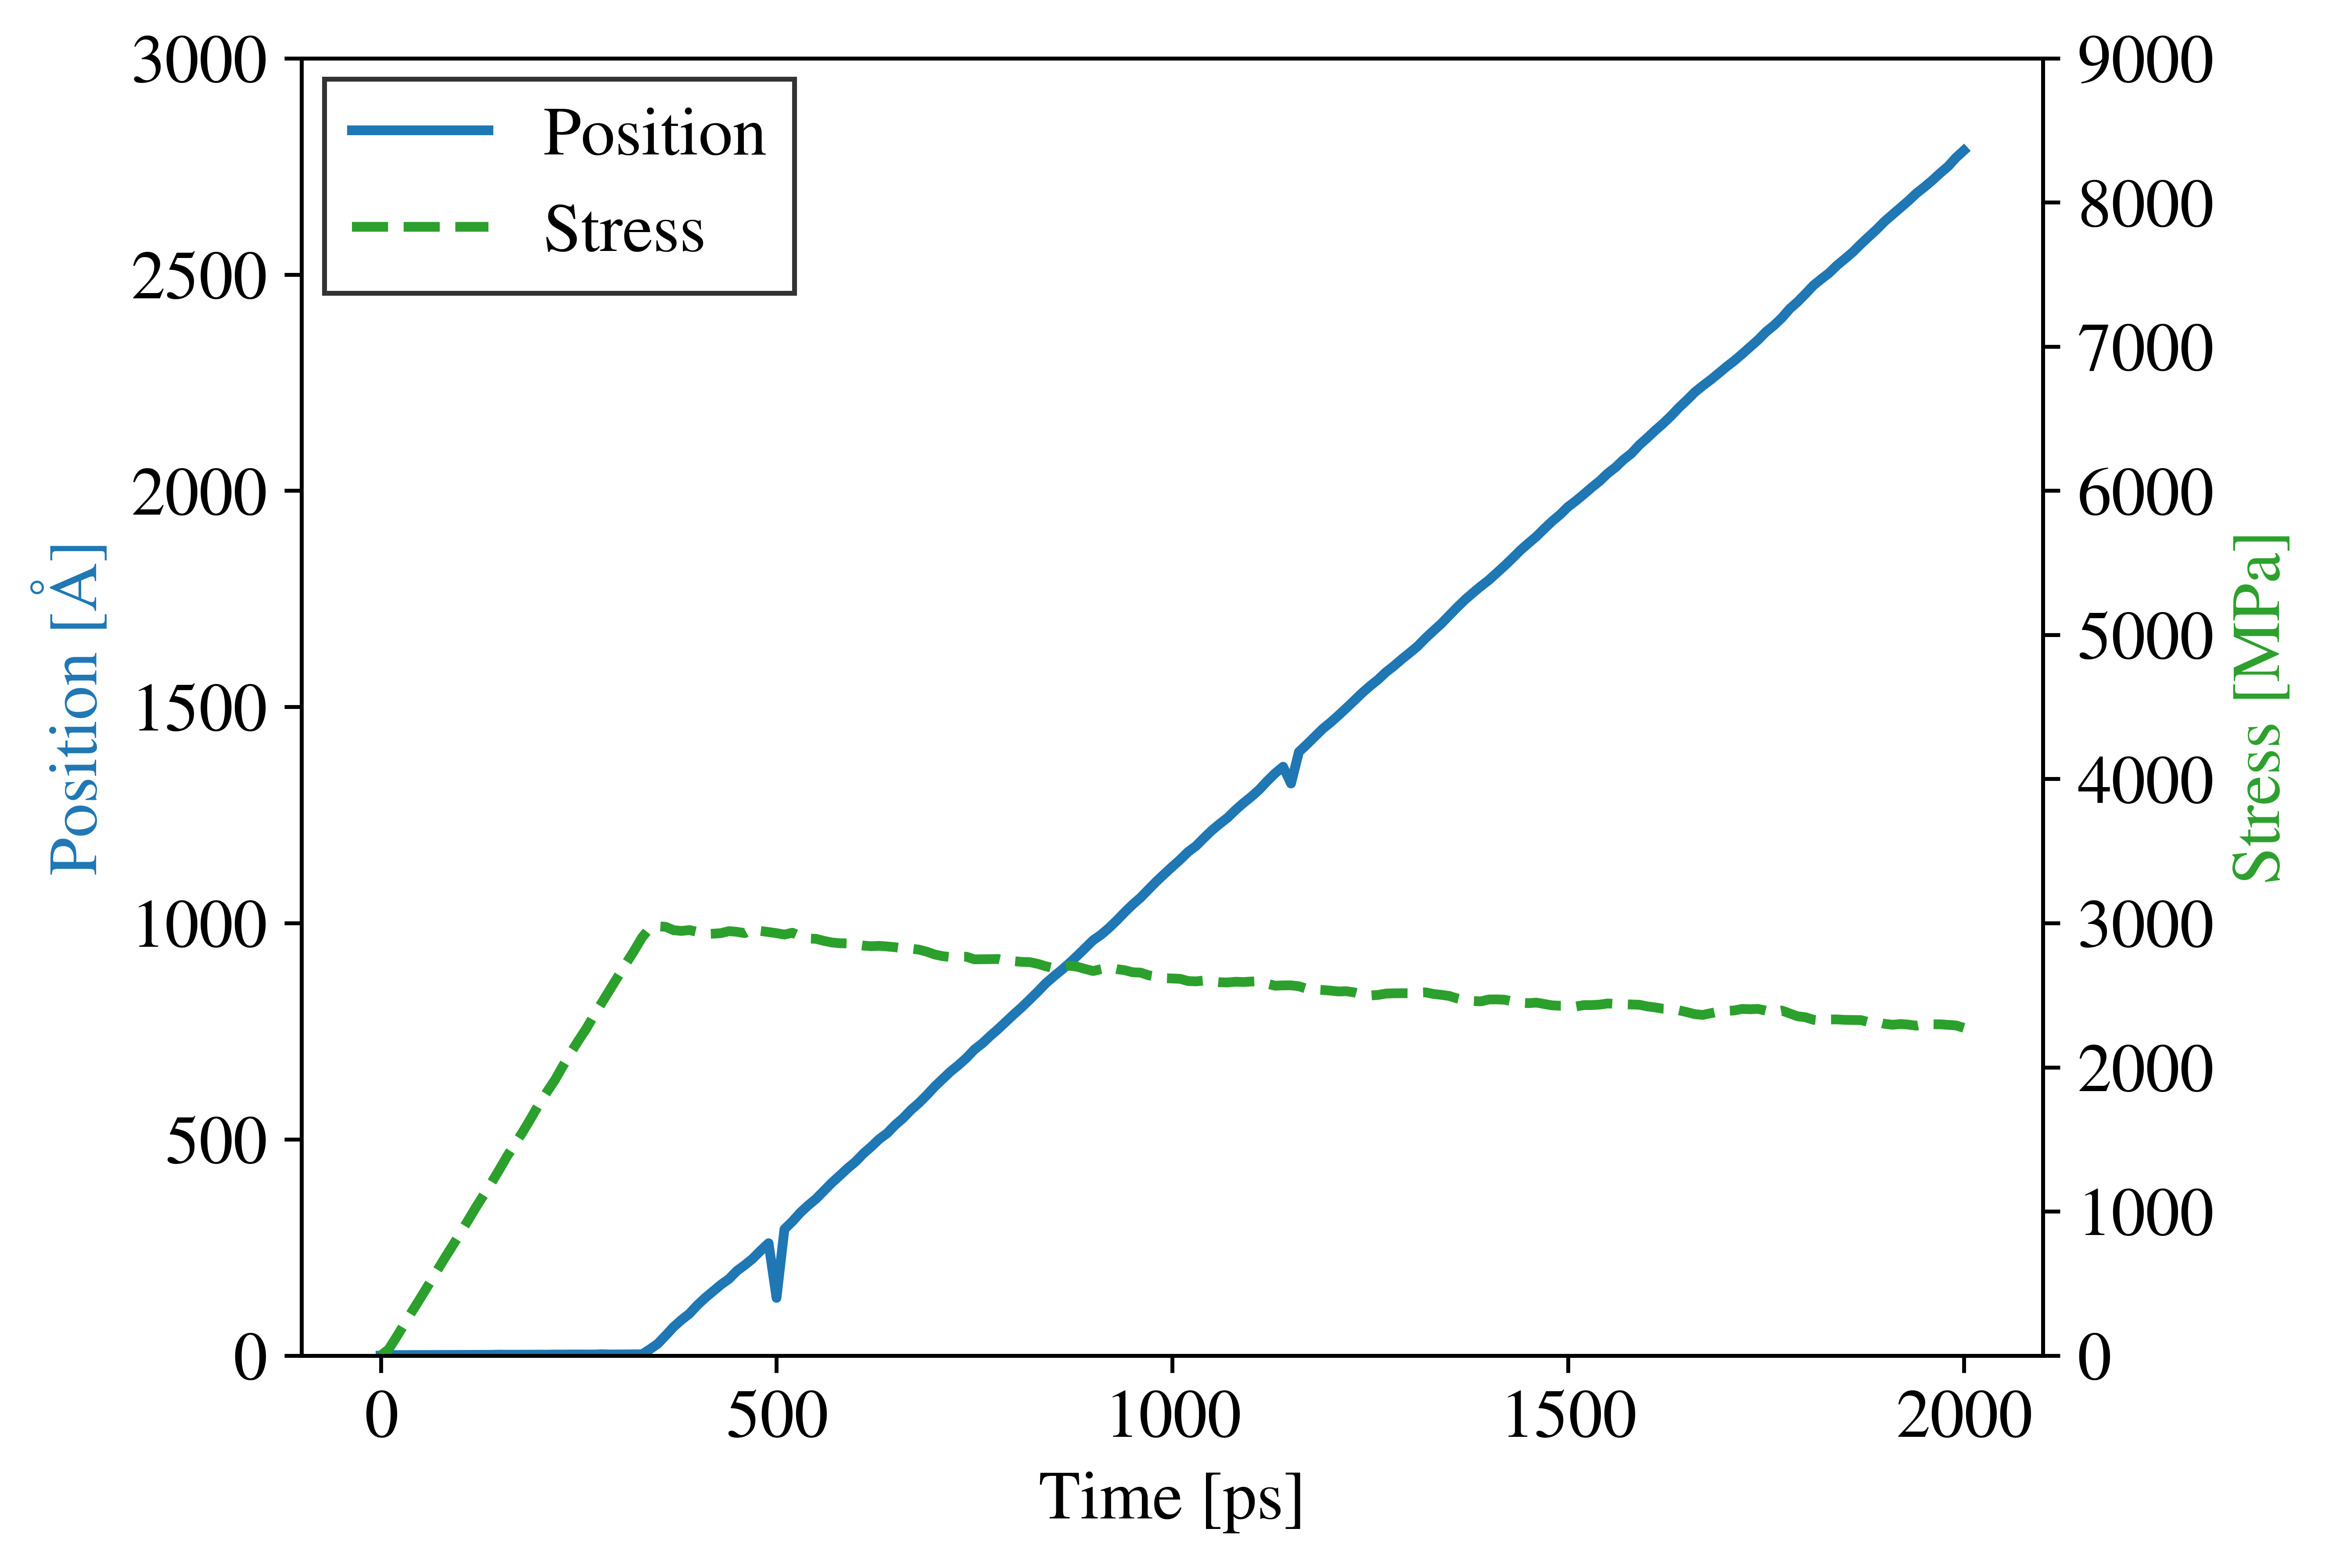
\includegraphics[width=0.48\textwidth]{Position-Stress-Edge111.png}}
\hfill
\subfloat[]{\label{Fig:Edge112}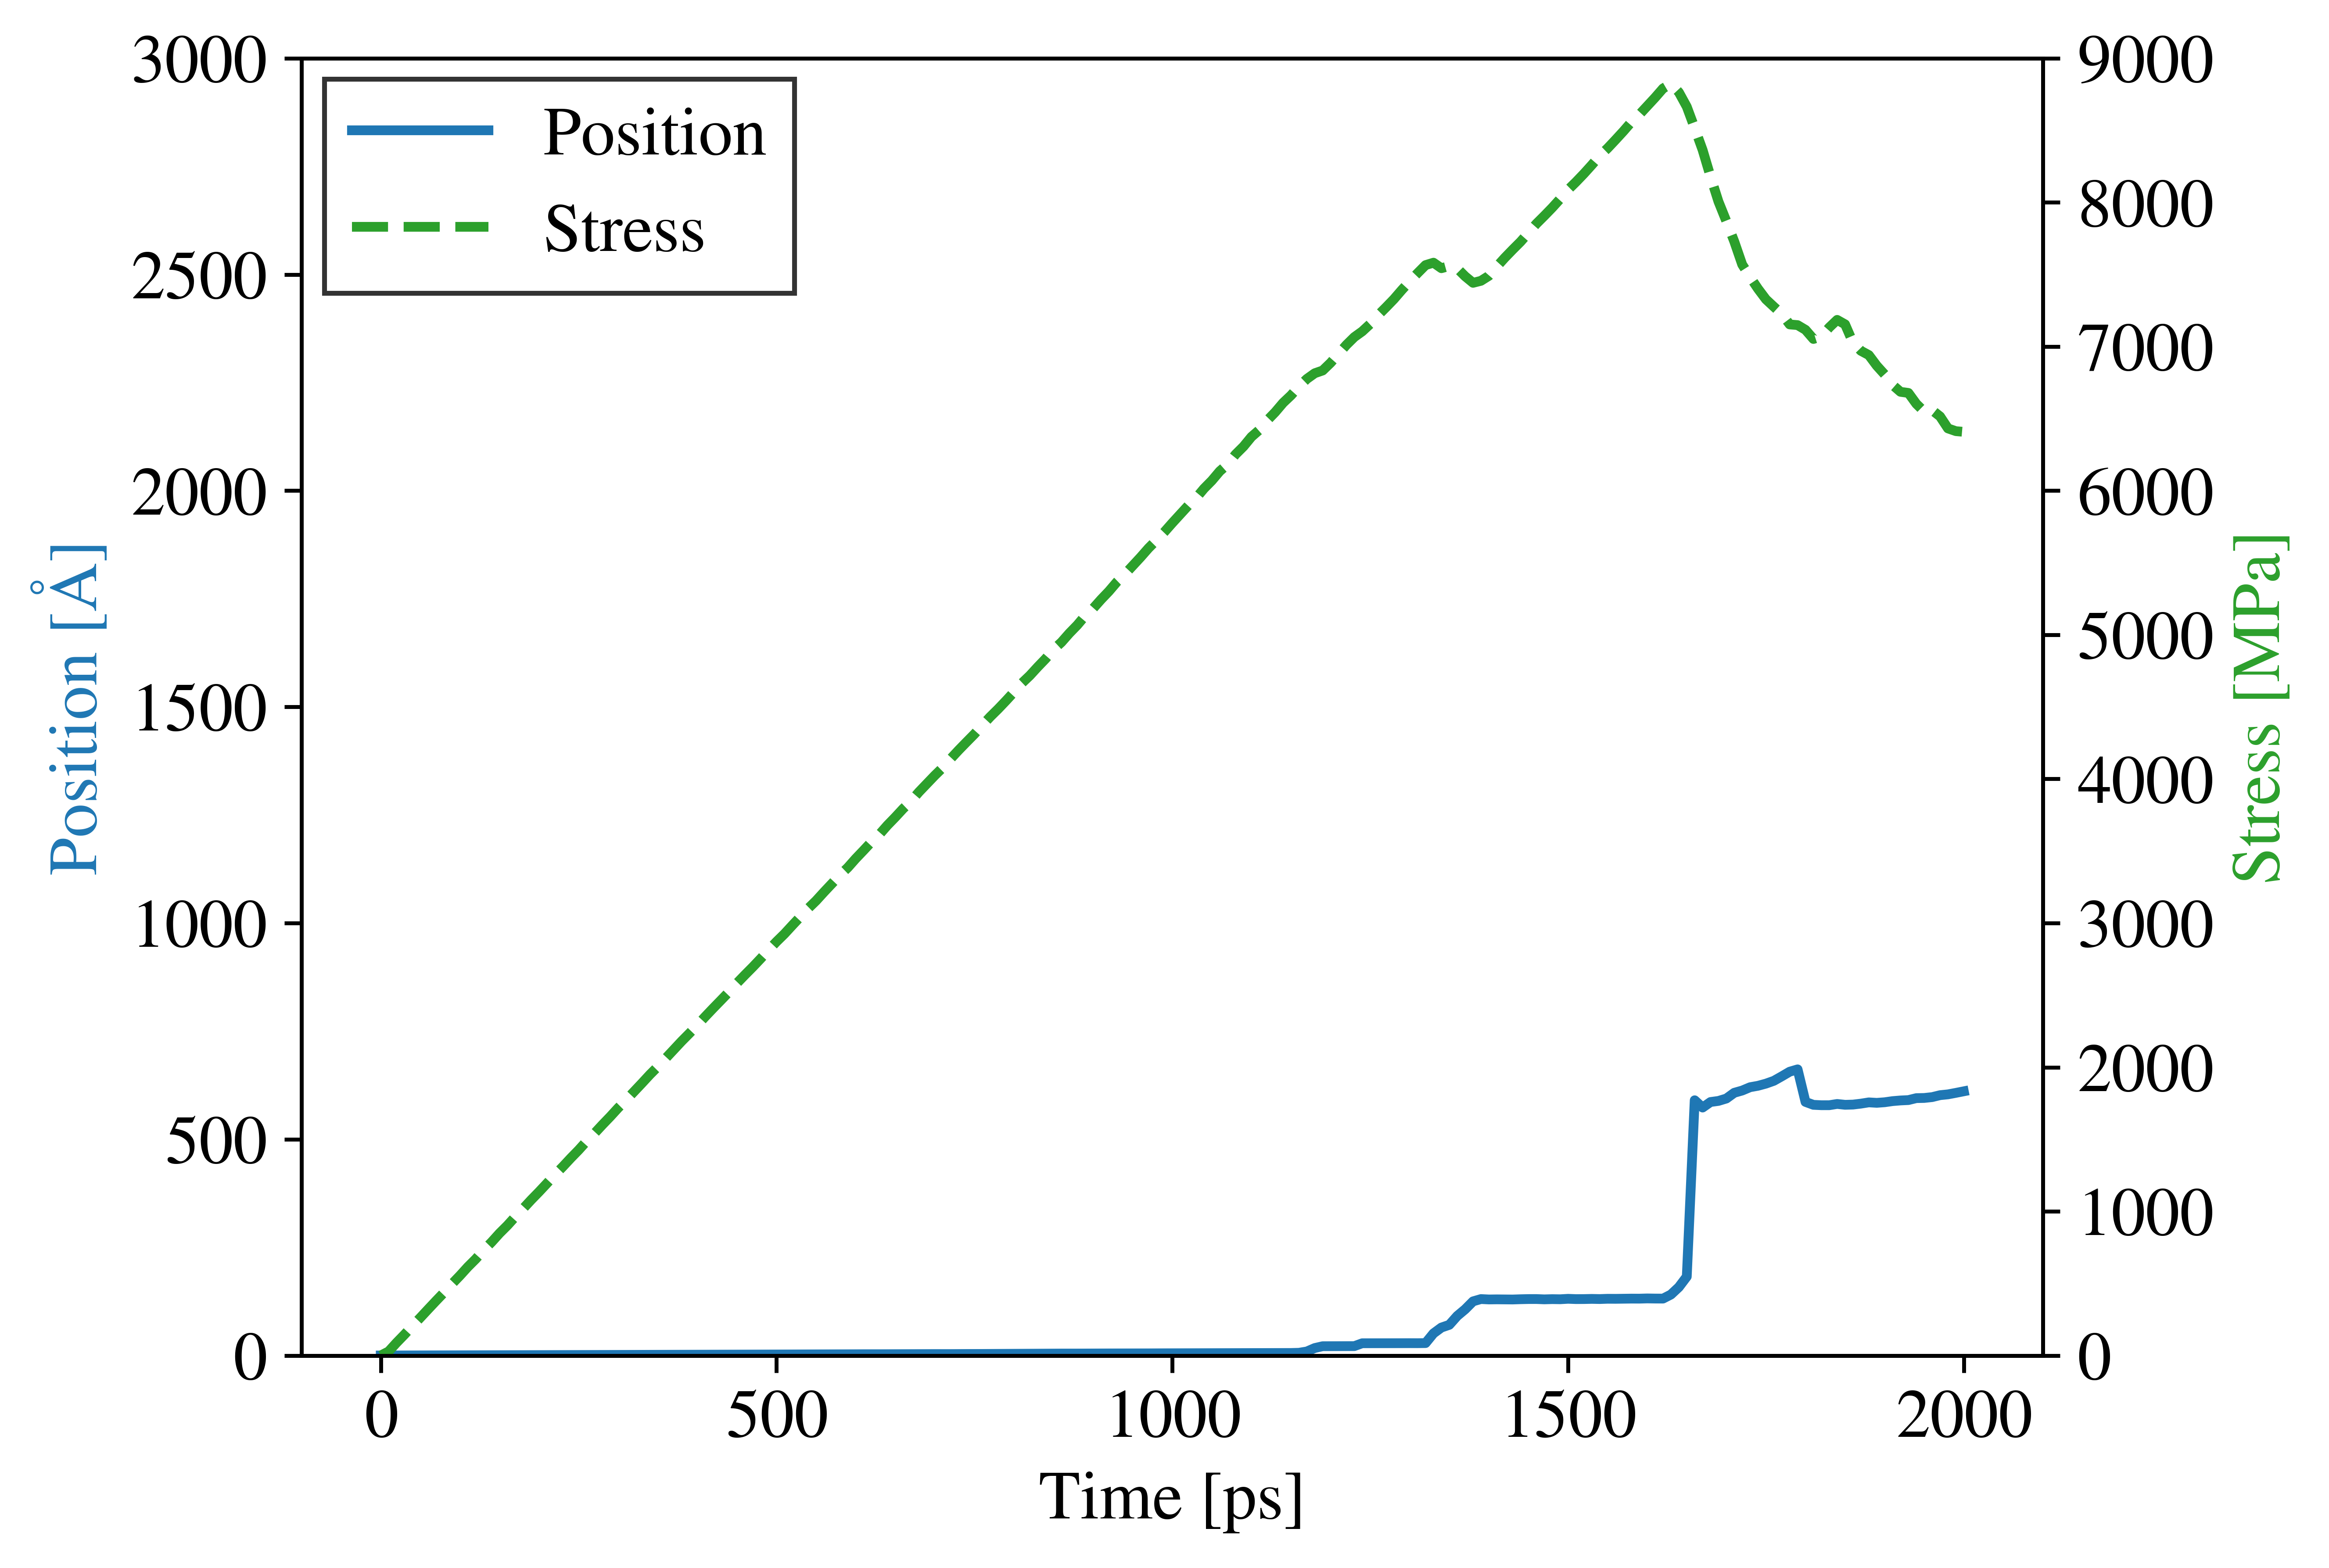
\includegraphics[width=0.48\textwidth]{Position-Stress-Edge112.png}}

\caption{(Color online) Movement of the $\frac{1}{2} \langle 110 \rangle$ edge dislocation along \textbf{(a)} $\{ 110 \}$, \textbf{(b)} $\{ 111 \}$, and \textbf{(c)} $\{112\}$ slip planes under applied strain rate of $10^{-4}$ s$^{-1}$. To calculate the Peierls stress, the developed shear stress on each dislocation is also averaged and shown in the figures.}
\label{Fig:Disloc}
\end{figure}

The displacement and stress of the $\frac{1}{2} \langle 110 \rangle$ edge dislocation as a function of time is shown in \cref{Fig:Disloc}. We can observe that the Peierls stress of the $\frac{1}{2} \langle 110 \rangle$ edge dislocation along the $\{ 111 \}$ plane is 2.98 GPa, whereas those for the $\{ 110 \}$ and $\{ 112 \}$ planes are 7.65 GPa and 8.82 GPa, respectively. This confirms that $\{ 111 \}$ is the principal slip plane in UN as predicted by the Tseplyaev potential because it requires the lowest stress for slip. It is also found that the $\{ 110 \}$ is predicted to be the second preferable slip plane. A Peierls stress of 2.98 GPa is on the order of 10$^{-2}$ $G$, $G \sim 100$ GPa being the shear modulus of UN as predicted by the Tseplyaev potential \cite{AbdulHameed2024}. This is the same order of magnitude of the Peierls stresses for purely covalent materials \cite{Hull2011}, which confirms our conclusion that the Tspelyaev potential very likely overestimates the covalency of the UN system. For purely ionic crystals like LiF and NaCl, the experimental values of the Peierls stress are $1.6 \times 10^{-4} G$, and $5.0 \times 10^{-4} G$, respectively \cite{Liu2012}.

Based on OVITO visualization, it was observed that the edge dislocation moves via a kink-pair mechanism \cite{Hull2011}. Assisted by thermal vibrations, the dislocation hops from one energy minimum to the next along the slip plane by forming unstable kink pairs, which then annihilate one another. This continuous kink-pair nucleation and annihilation process reduces the threshold stress required to move the dislocation much below the Peierls stress. Although the kink-pair nucleation mechanism at very low stresses is often observed for screw dislocations and rarely for edge dislocations due to stress fluctuations \cite{Gilbert2011, Starikov2020}, it has been observed in the atomistic simulations by Yu \textit{et al.} \cite{Yu2009b} for edge dislocations in $\alpha$-Fe.

\begin{figure}[h!]
\centering
\subfloat[]{\label{Fig:DislocMob1}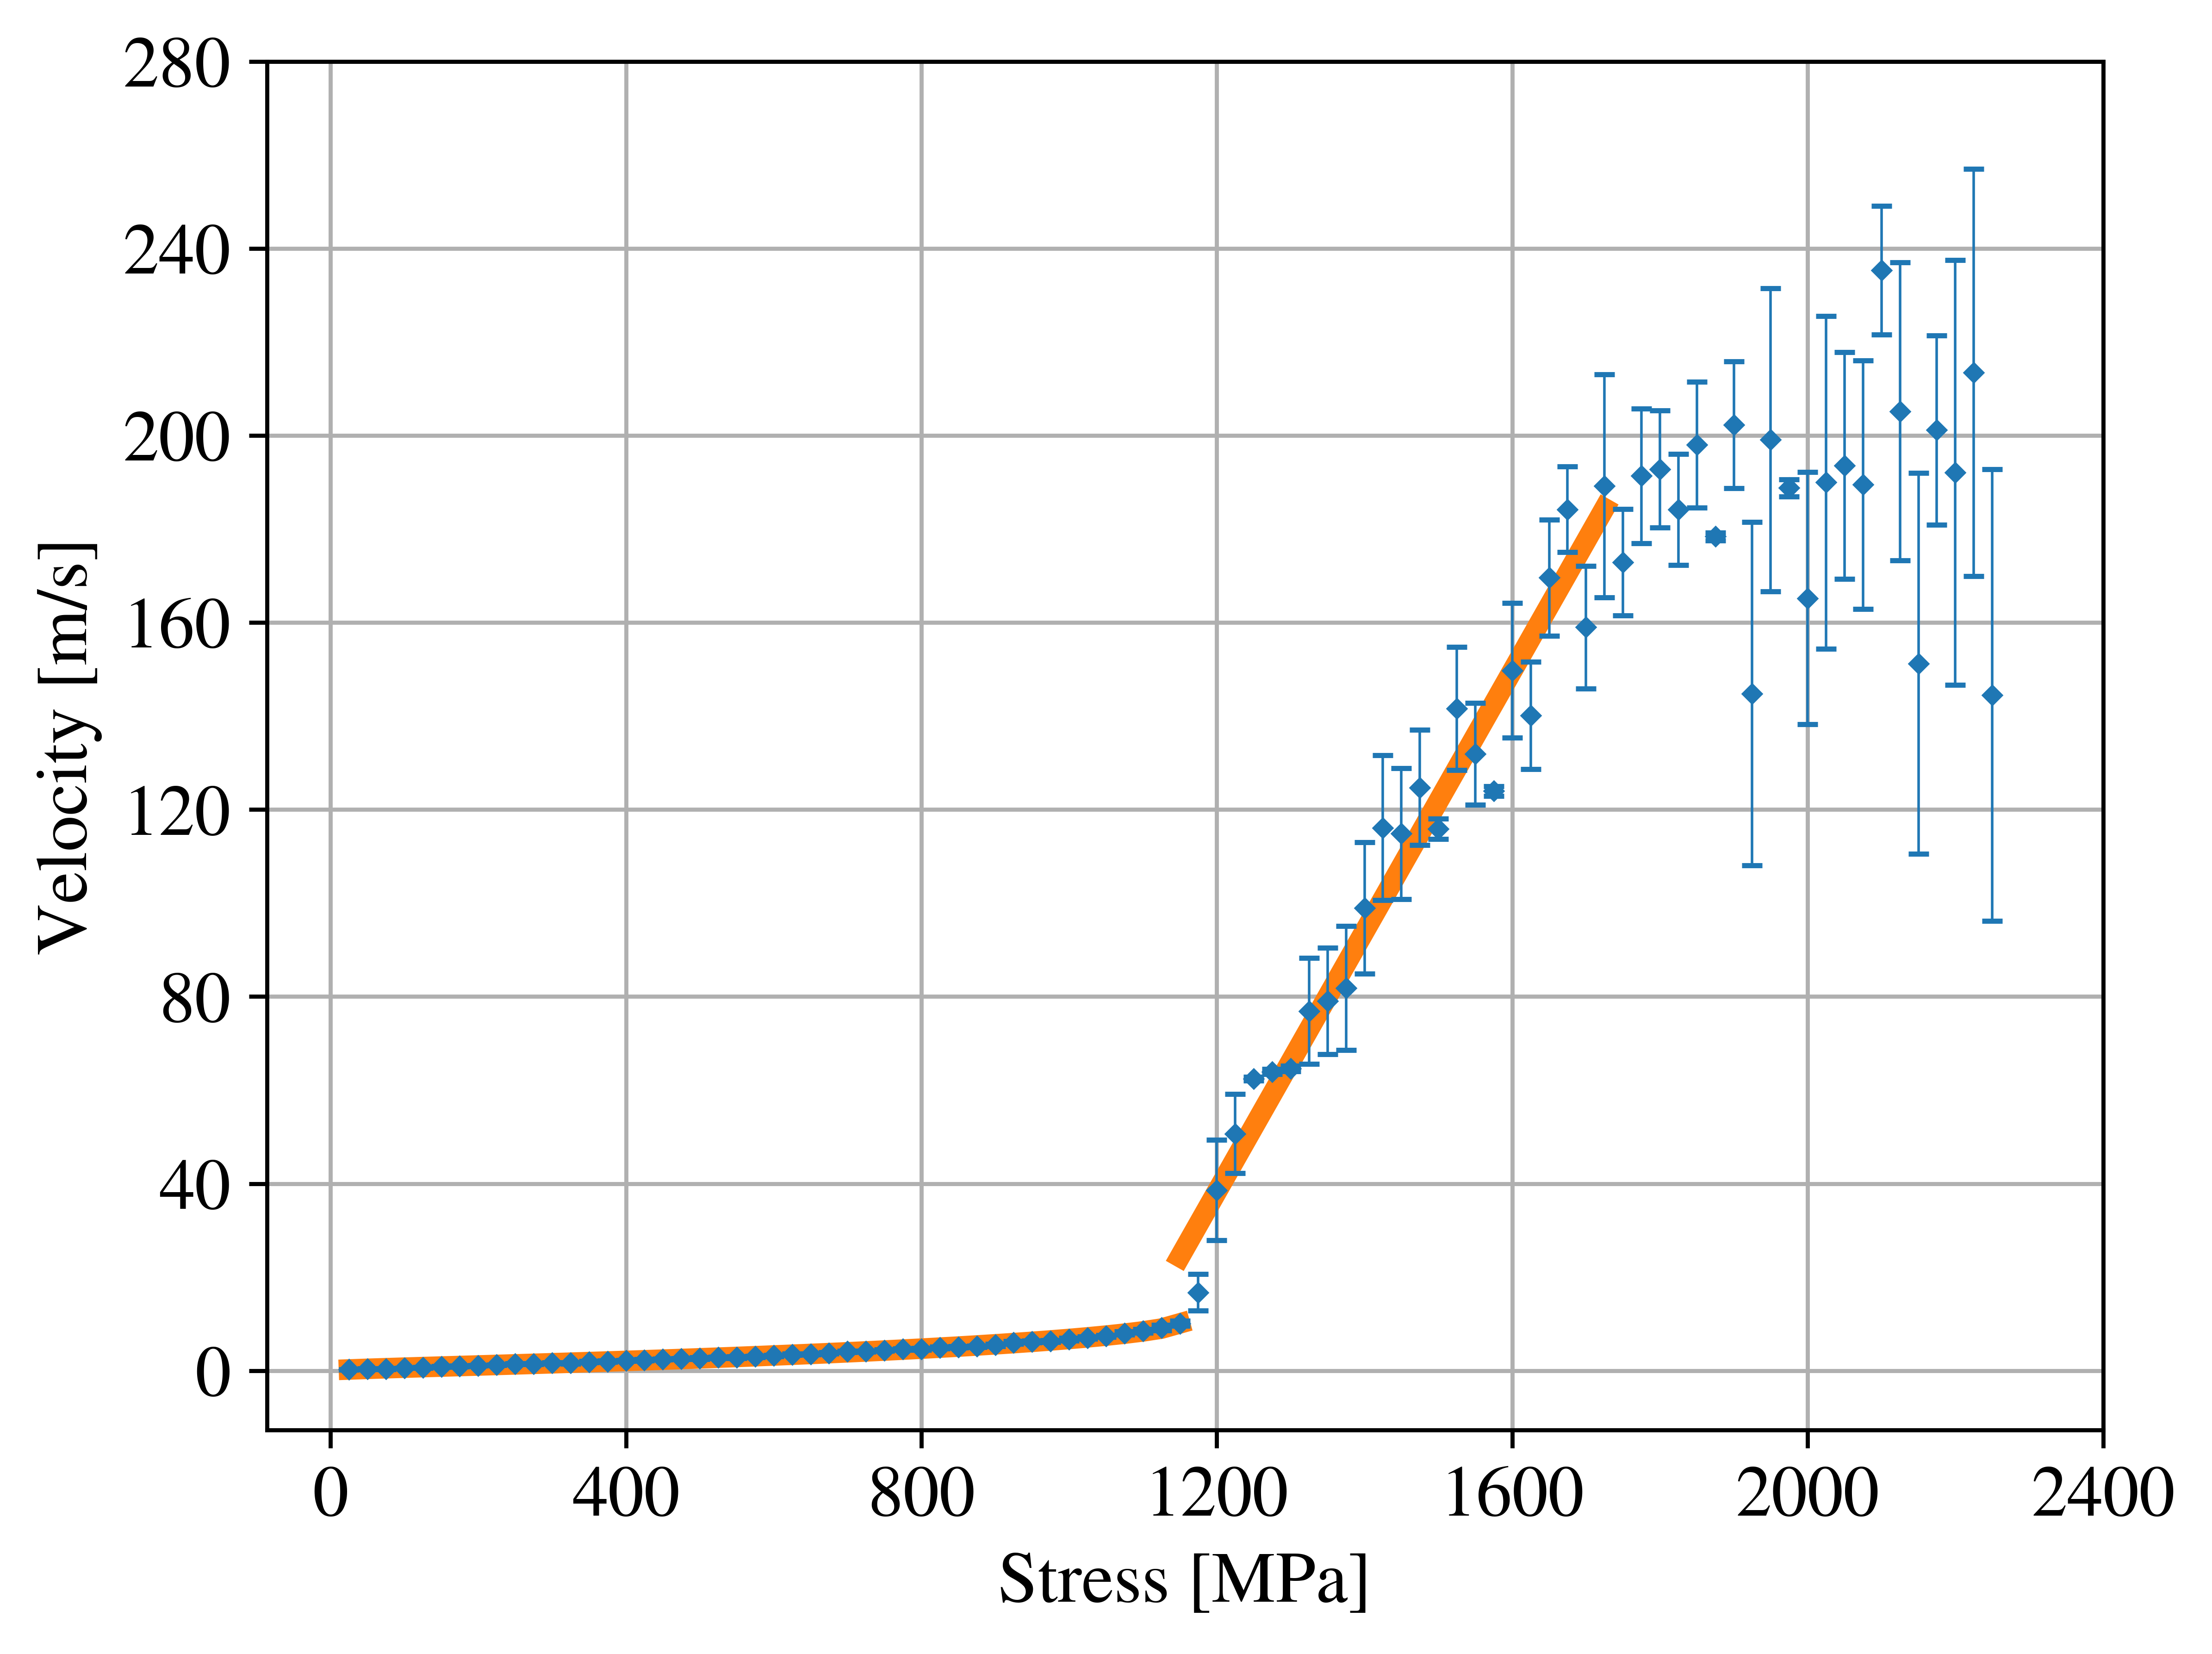
\includegraphics[width=0.48\textwidth]{DislocMob1.png}}
\hfill
\subfloat[]{\label{Fig:DislocMob2}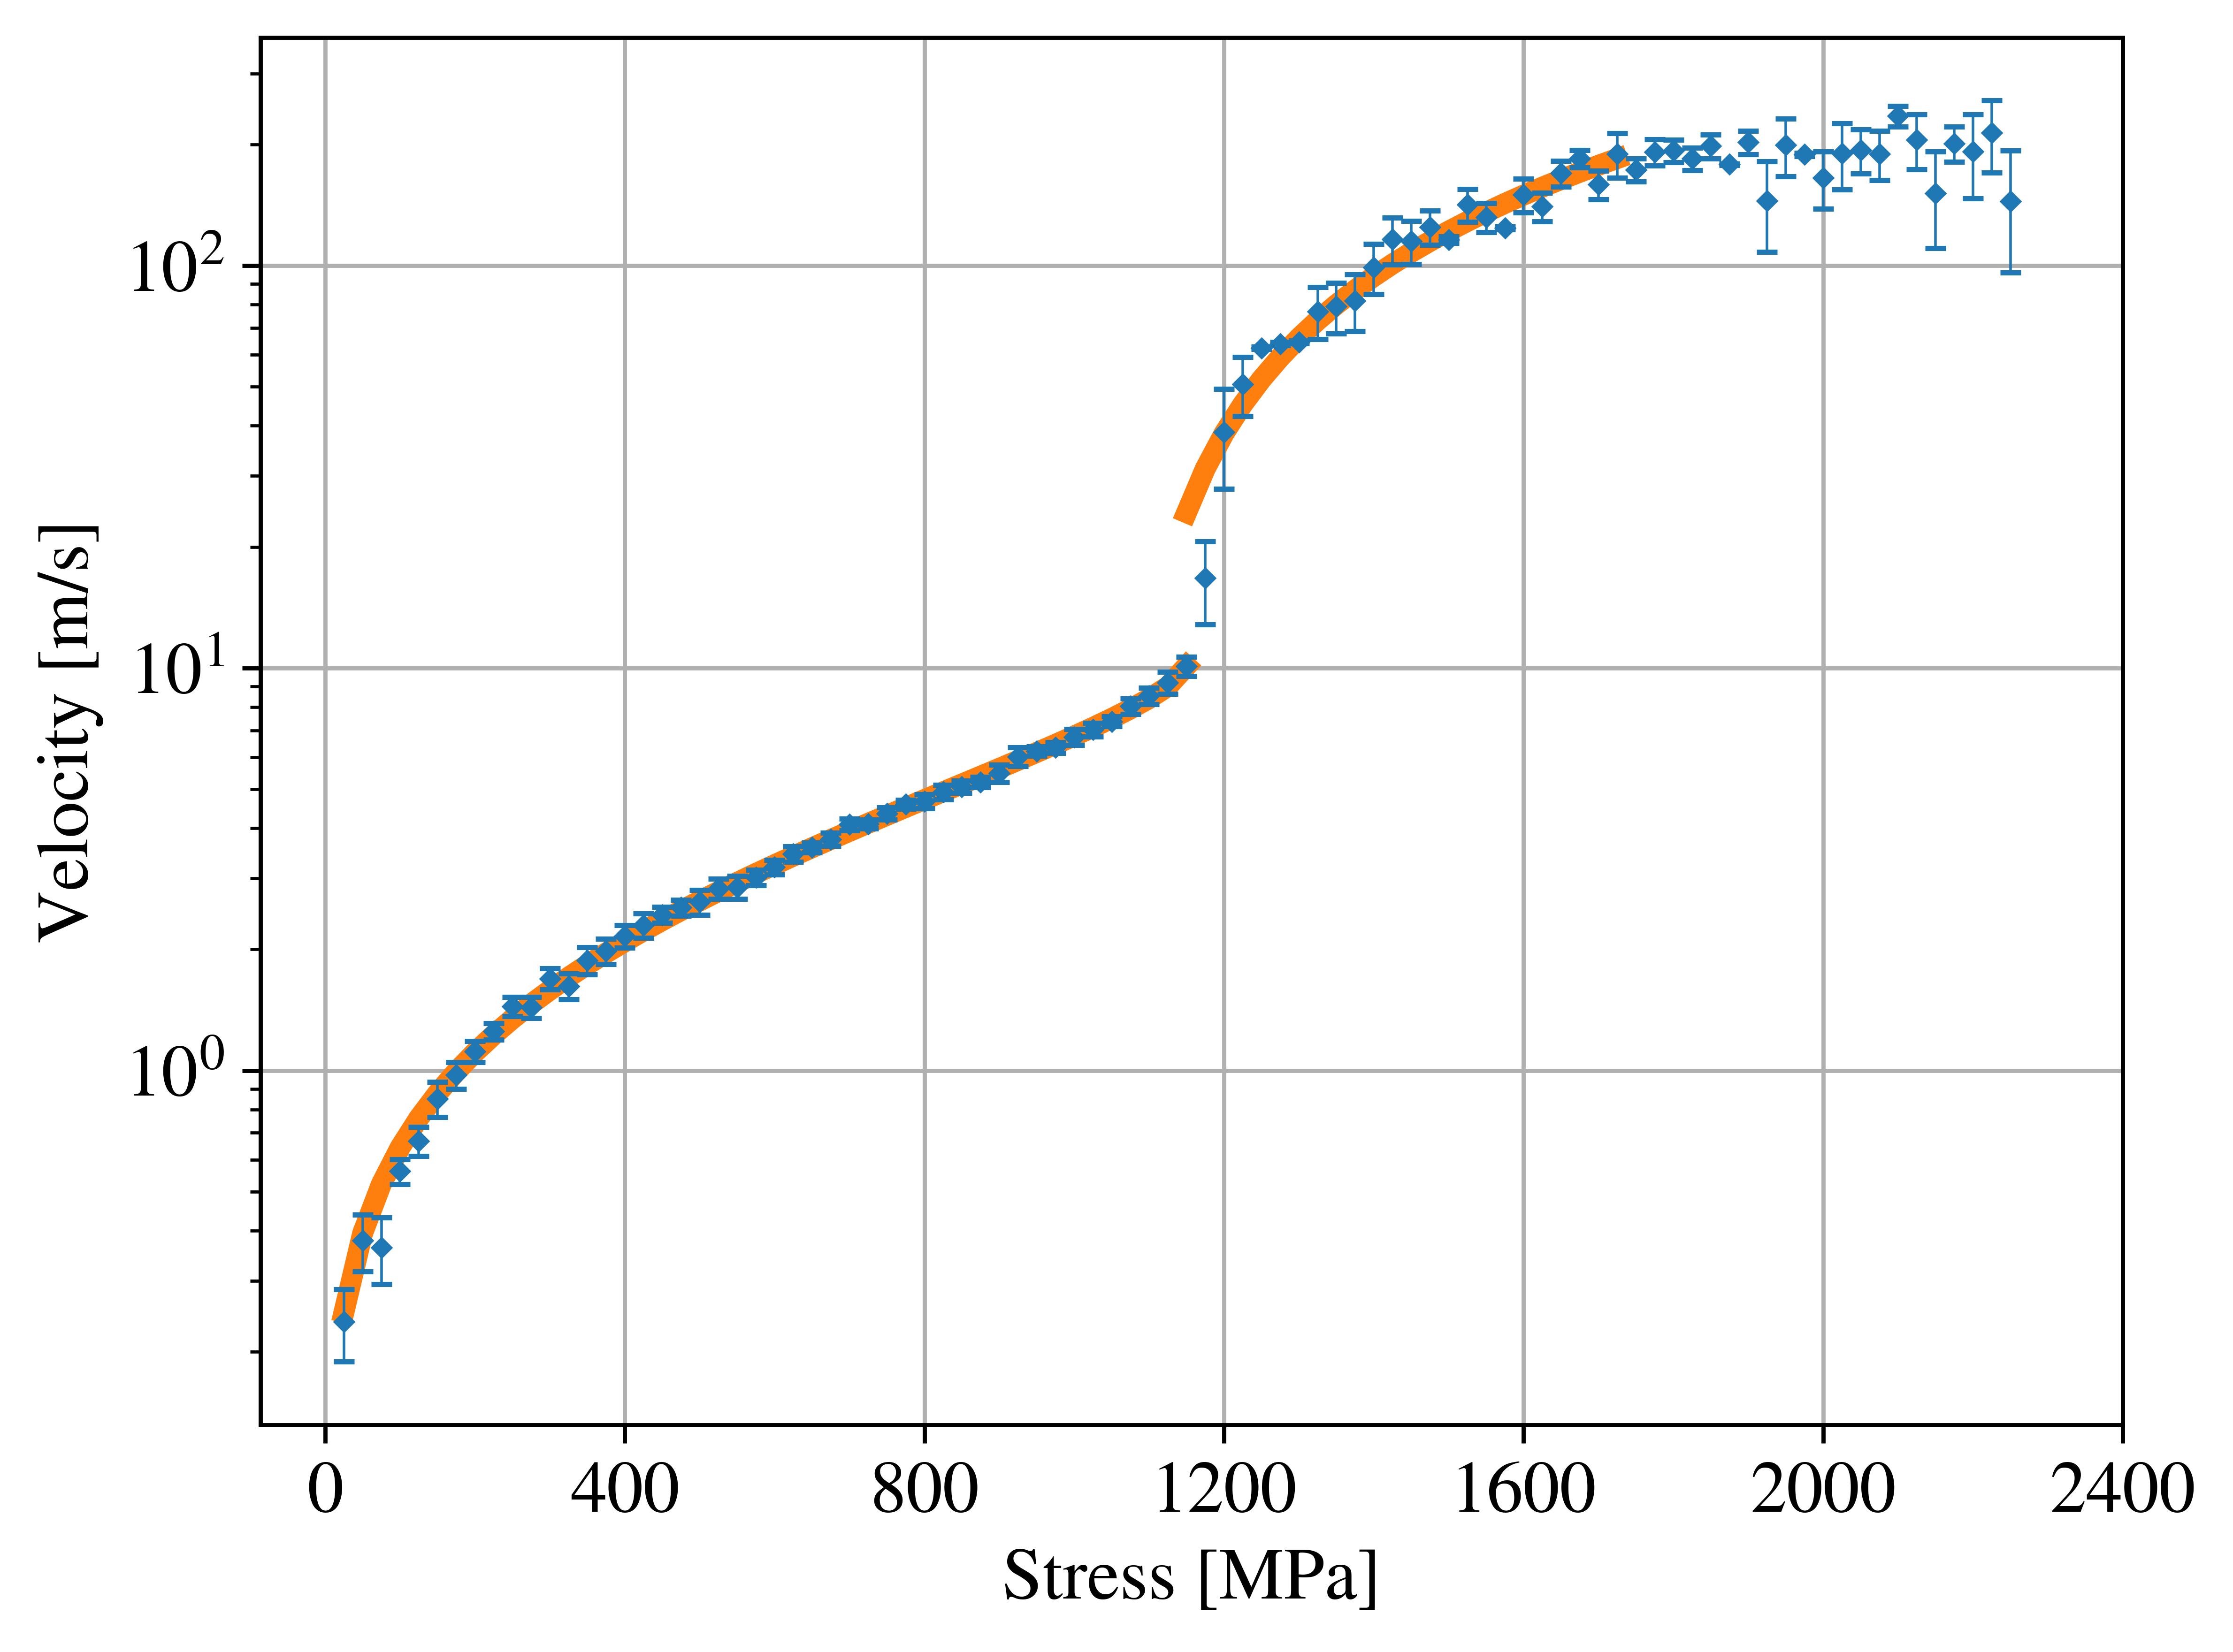
\includegraphics[width=0.48\textwidth]{DislocMob2.png}}
\caption{The variation of the average edge dislocation velocity in UN with shear stress \textbf{(a)} on a linear scale, and \textbf{(b)} on a semi-log scale. The error bars represent one standard deviation, and the orange lines represent piecewise curve fits.}
\label{Fig:DislocPosTime}
\end{figure}

Due to the probabilistic nature of dislocation hopping, at relatively low stresses ($\tau \leq 1150$ MPa) the motion is dominated by fluctuations and no steady-state velocity can be observed. When the stress is increased, fewer fluctuations are observed and a nearly steady-state velocity emerges. To be consistent, however, we calculate the velocity at all stresses as the total distance traveled divided by the total simulation time, i.e., 1 ns. The variation of dislocation velocity with the applied shear stress at 300 K is shown in \cref{Fig:DislocMob1} on a linear scale and \cref{Fig:DislocMob2} on a semi-log scale which is introduced to clarify the velocity trend at Regime I. The parameters resulting from fitting the velocity-stress curve to \cref{Eq:MobI,Eq:MobII} are summarized in \cref{Tab:DislocParams}. For the stress range of 25--1150 MPa (i.e., Regime I), the velocity-stress curve has been fitted to \cref{Eq:MobI} with $H_0 = 0.11$ eV, $p=0.37$, and $q=0.62$. The transition velocity was identified as $v_t$ = 10.1 m/s, which is the velocity corresponding to the transition stress $\tau_t$ = 1150 MPa. These values produced $R^2 = 99.9\%$. A value of $H_0 = 0.11$ eV for UN is reasonable considering that the experimental values of the same parameter for LiF, NaCl, and KCl are 0.09, 0.11, and 0.16 eV, respectively \cite{Haasen1985}. Kink-pair formation energies are sensitive to supercell dimensions, especially the dimension along the dislocation line \cite{Ventelon2009}. Thus, the calculated value of $H_0$ should be treated as a first estimate, and more research is required to test its convergence. A value of $p = 0.37$ falls within the expected range (i.e., $0 \leq p \leq 1$). The value of $q = 0.62$, however, is slightly underestimated relative to the expected range (i.e., $1 \leq q \leq 2$).

\begin{table}[h!]
\centering
\caption{Parameters of the mobility functions (\cref{Eq:MobI,Eq:MobII}) fitted to the motion of the $\frac{1}{2}\langle110\rangle\{111\}$ edge and $\frac{1}{2}\langle110\rangle\{110\}$ screw dislocations at 300 K.}
\footnotesize
\begin{tabular}{lll}
\hline
Parameter & Edge dislocation & Screw dislocation \\
\hline
Kink-pair formation energy, $H_0$ [eV] & 0.11 & 1.0 \\
Exponent $p$ & 0.37 & 0.0037 \\
Exponent $q$ & 0.62 & 0.30 \\
Transition stress between Regimes I and II, $\tau_t$ [MPa] & 1150 & 700 \\
Transition velocity between Regimes I and II, $v_t$ [m/s] & 10.1 & 20.1 \\
Phonon drag coefficient, $B$ [$\mathrm{Pa} \! \cdot \! \mathrm{s}$] & $1.22 \times 10^{-3}$ & $2.20 \times 10^{-4}$ \\ 
Mobility, $M$ [$\mathrm{Pa}^{-1} \! \cdot \! \mathrm{s}^{-1}$] & 817 & 4546 \\
Additive constant $C$ [m/s] & $-296$ & $-1134$ \\
Transition stress between Regimes II and III, $\tau_t'$ [MPa] & 1725 & 1125 \\
\hline
\end{tabular}
\label{Tab:DislocParams}
\end{table}

At a stress of $\tau_t$ = 1150 MPa, a transition to Regime II occurs where the velocity varies linearly with stress. Fitting the velocity-stress curve in Regime II to \cref{Eq:MobII}, we find that the phonon drag coefficient $B$ = $1.22 \times 10^{-3}$ $\mathrm{Pa} \! \cdot \! \mathrm{s}$. This value produces $R^2 = 95.8\%$. The linear fit is valid until a stress $\tau_t'$ = 1725 MPa where a deviation from linearity is apparent, i.e., a transition to Regime III occurs where the uncertainty in the velocity is much higher than in Regimes I and II with a maximum standard deviation of 50 m/s. The linear dislocation mobility is calculated to be $M = 1/B$ = 817 $\mathrm{Pa}^{-1} \! \cdot \! \mathrm{s}^{-1}$. To give context to this value, the mobility of edge dislocations in \ce{Fe40Cr25Ni35} and \ce{Fe50Cr20Ni30} steel systems was calculated by Kaloni \textit{et al.} \cite{Kaloni2023} to be $5.01 \times 10^4$ and $7.04 \times 10^4$ $\mathrm{Pa}^{-1} \! \cdot \! \mathrm{s}^{-1}$, respectively. This implies that UN is less ductile than steel systems, which is expected considering that UN is ceramic.

An interesting observation is that in the linear range at intermediate stresses, the steady-state movement of the dislocation is occasionally interrupted by abrupt jumps that occur within a small time interval of 20 ps as shown in \cref{Fig:Velocity-1525-MPa} for $\tau$ = 1525 MPa. These jumps have a velocity of 2977 $\pm$ 32 m/s independent of the applied stress. This velocity compares very well with the UN average sound velocity of 2990 m/s \cite{Baranov2013}. While it is observed experimentally that dislocations move with the sound velocity at very high stresses \cite{Johnston1959}, our finding suggests that at intermediate stresses, even when the edge dislocation displays a subsonic behavior, its steady-state motion can be interrupted by jumps that have a maximum velocity equal to the average sound velocity. This agrees with the picture that dislocation motion is stochastic.

\begin{figure}[h!]
\centering
\subfloat[]{\label{Fig:Velocity-1525-MPa}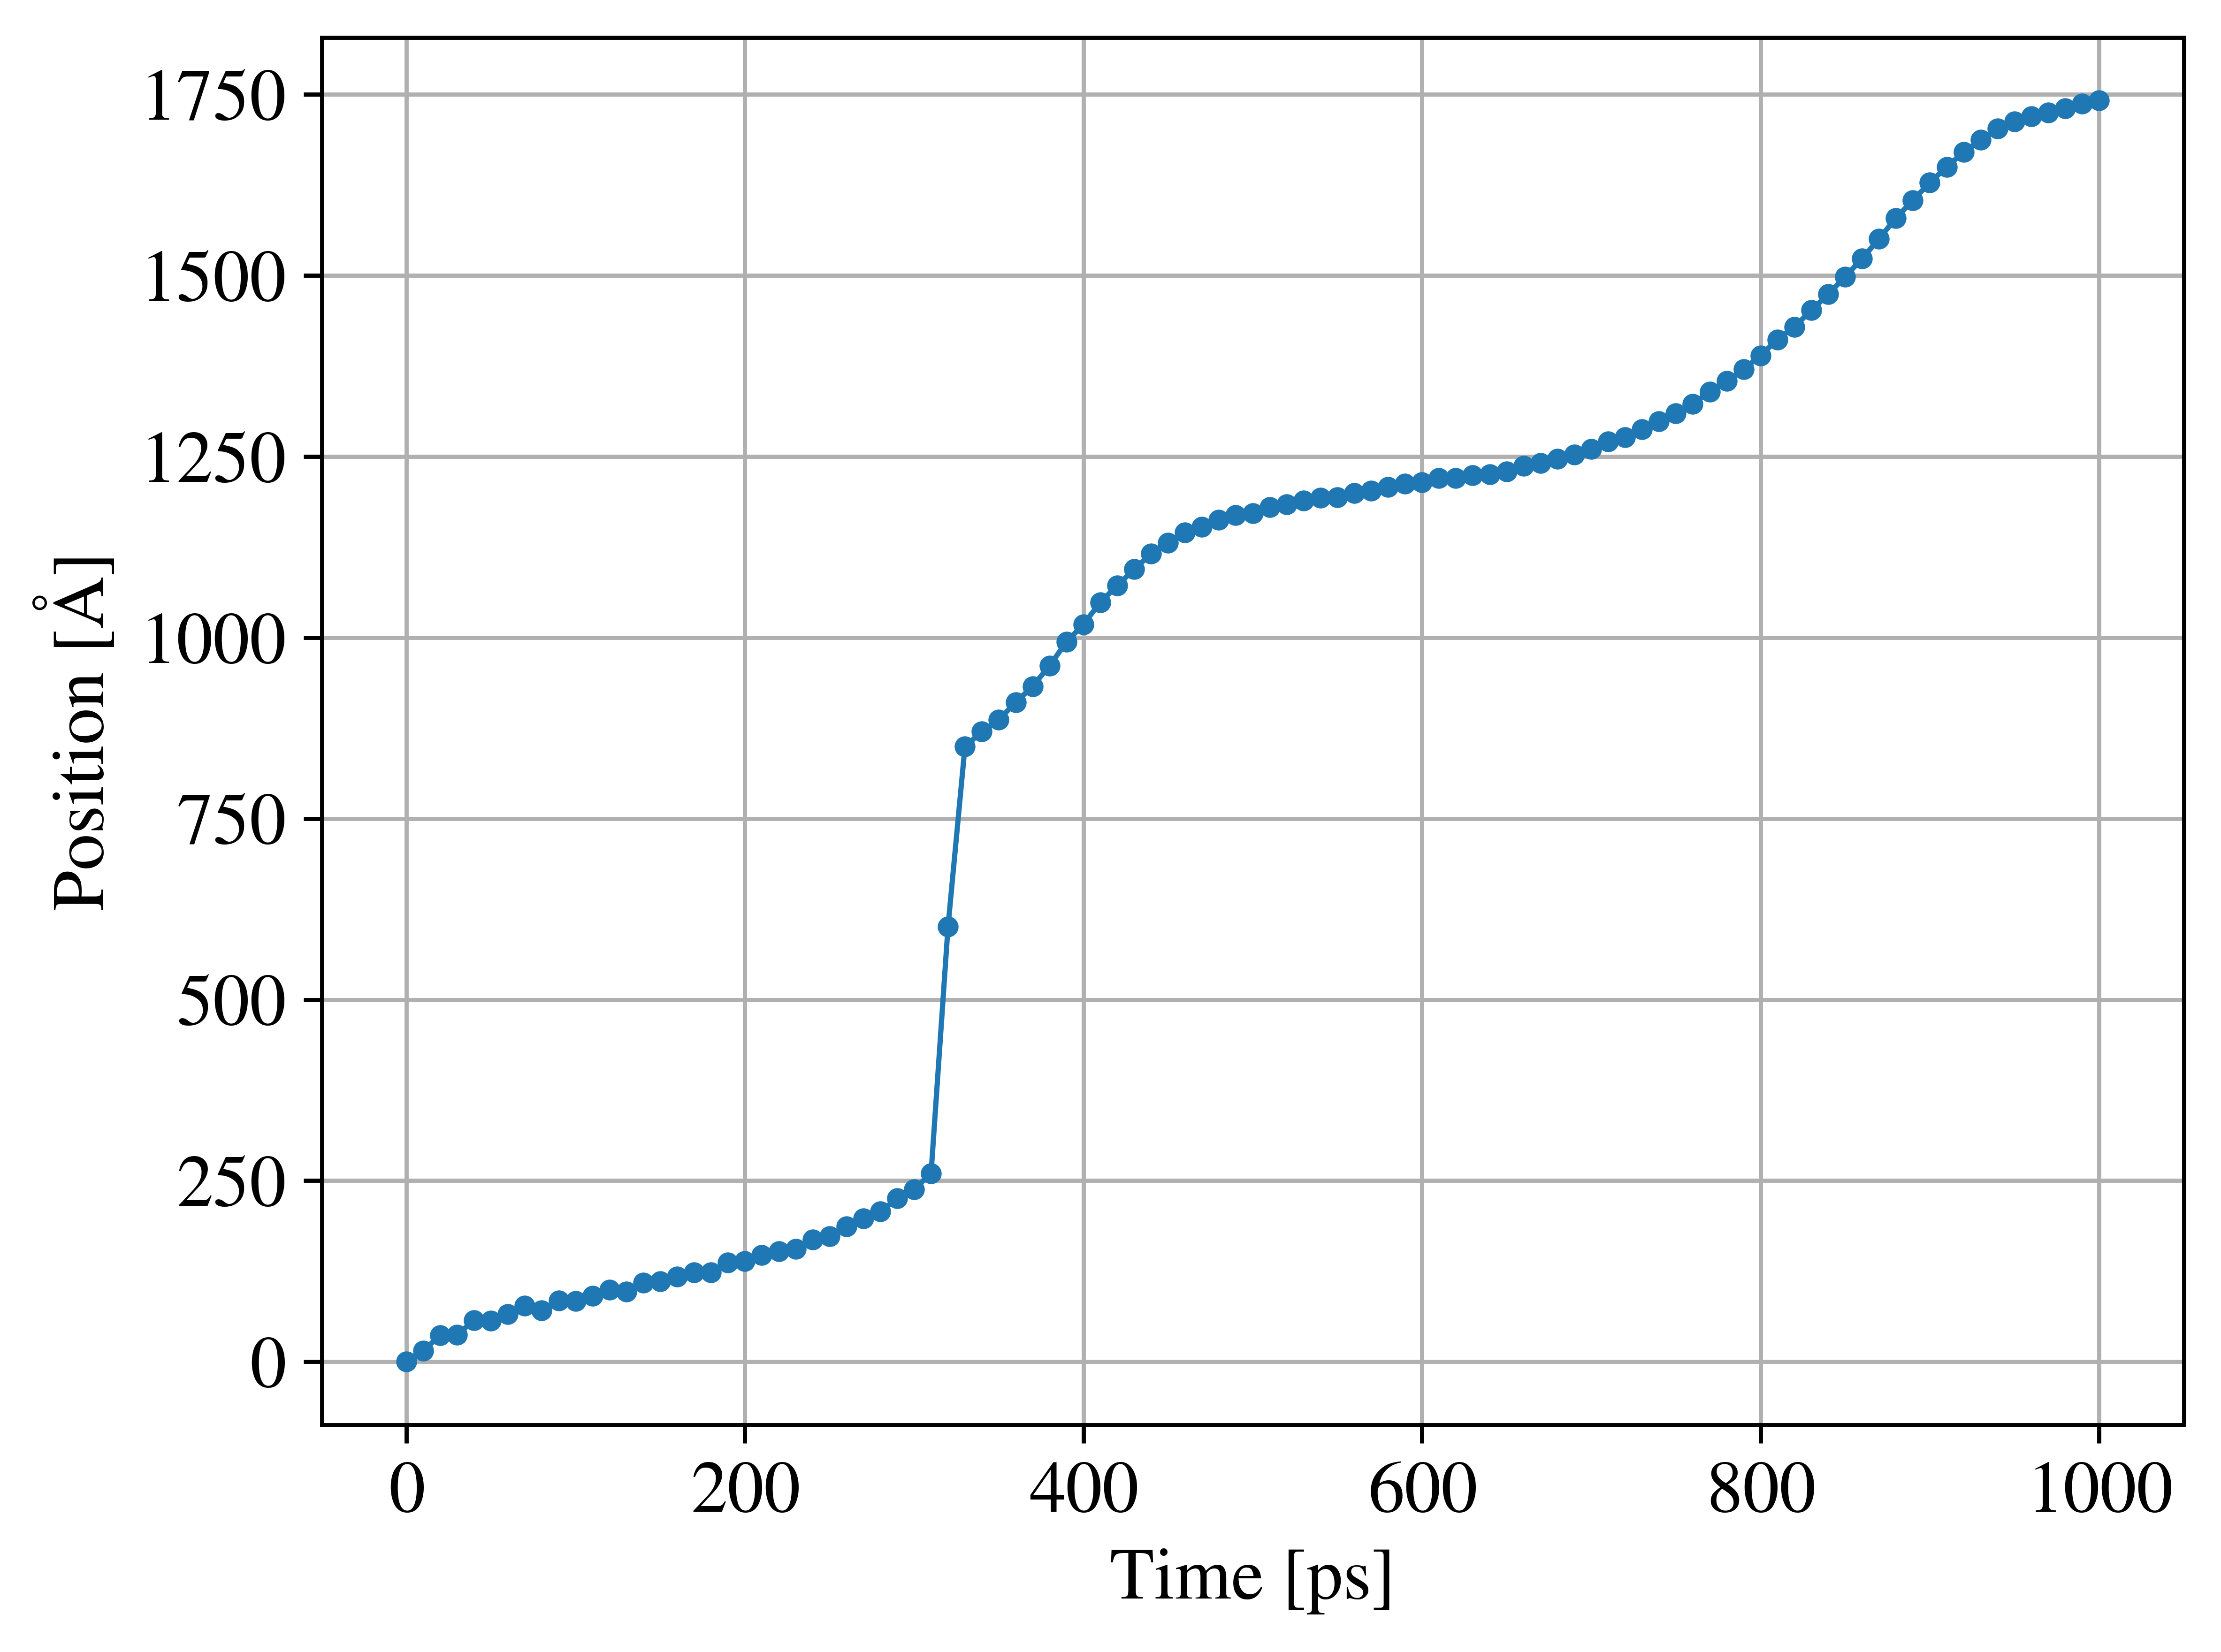
\includegraphics[width=0.48\textwidth]{Velocity-1525-MPa.png}}
\hfill
\subfloat[]{\label{Fig:Velocity-1000-MPa}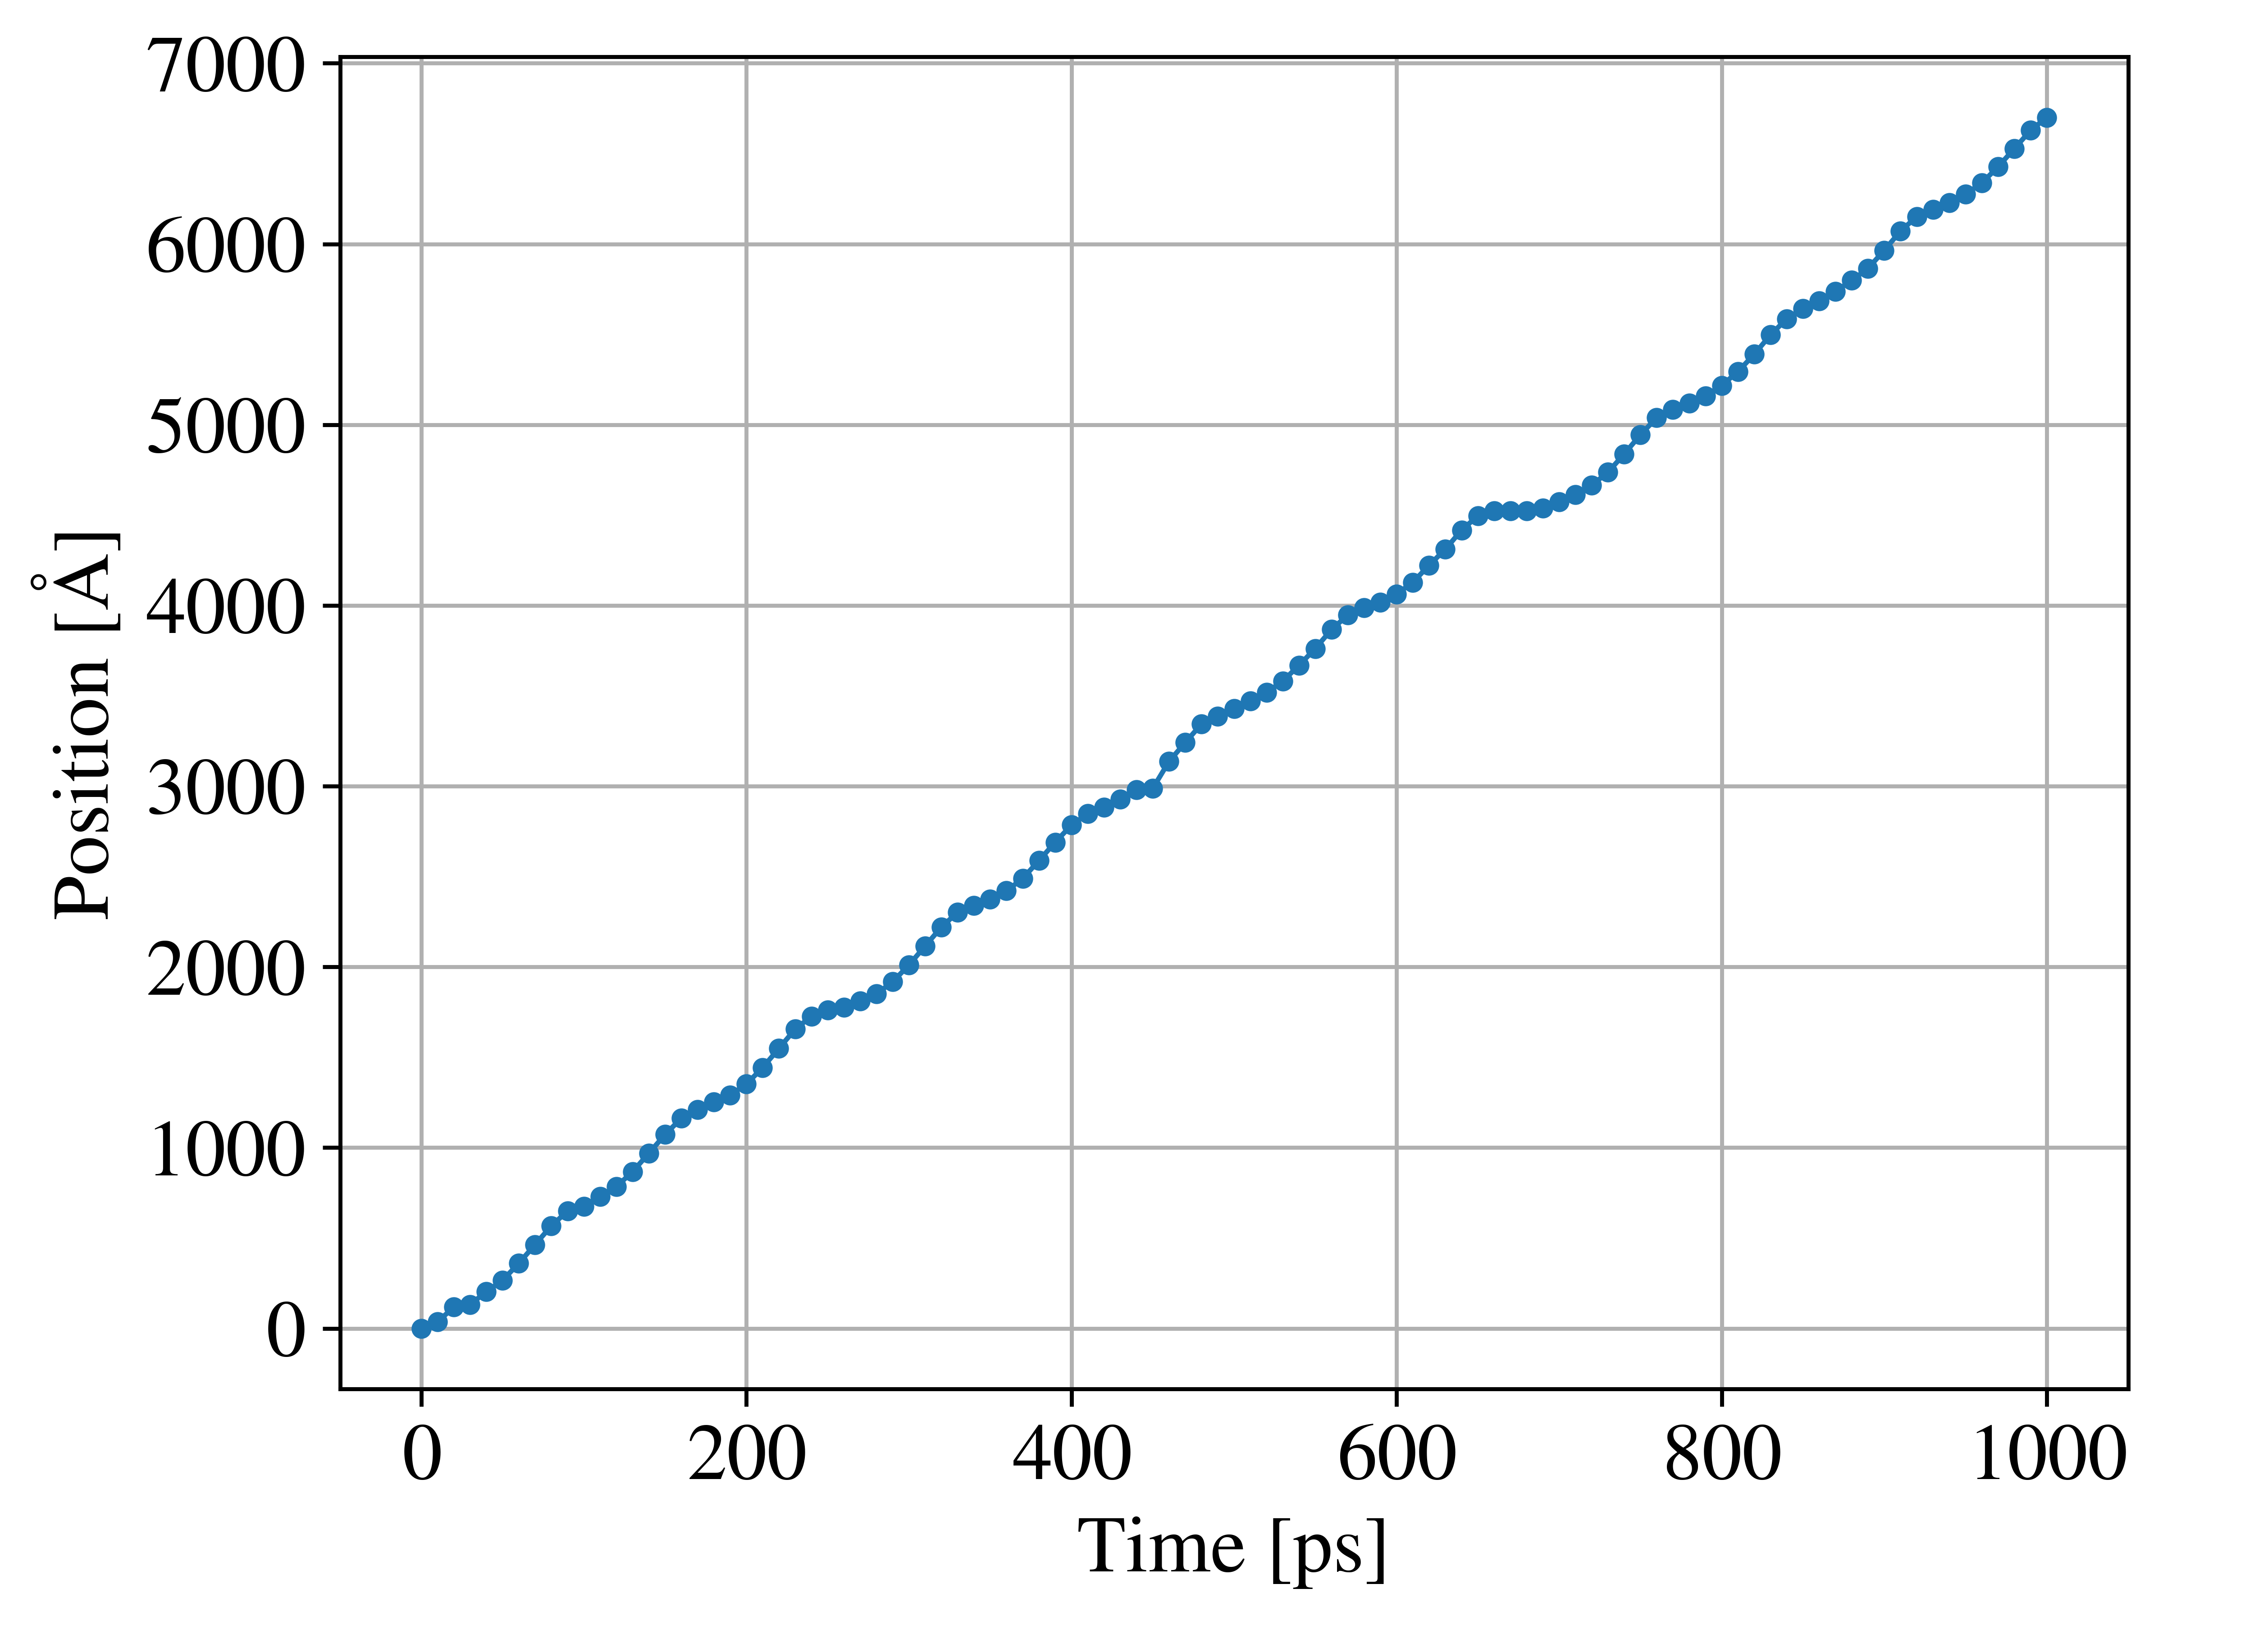
\includegraphics[width=0.48\textwidth]{Velocity-1000-MPa.png}}

\caption{\textbf{(a)} Position versus time profile for the movement of the $\frac{1}{2} \langle 110 \rangle \{ 111 \}$ edge dislocation under a stress of 1525 MPa. \textbf{(b)} Position versus time profile for the movement of the $\frac{1}{2} \langle 110 \rangle \{ 110 \}$ screw dislocation under a stress of 1000 MPa.}
\label{}
\end{figure}

\subsubsection{Screw dislocations}

For the screw dislocations simulated using the Kocevski potential, we aimed to calculate the Peierls stress at 1 K for the $\{110\}$, $\{111\}$, and $\{112\}$ planes. The $\frac{1}{2} \langle 110 \rangle$ screw dislocation moved smoothly along the $\{110\}$ plane, as illustrated in \cref{Fig:Screw1K}. When the dislocation was set to move along the $\{111\}$ and $\{112\}$ planes using the Kocevski potential, it was observed to cross-slip onto planes that form angles of 35.3$^\circ$ and 54.7$^\circ$ with the $\{111\}$ and $\{112\}$ planes, respectively. These angles precisely correspond to the angles between these planes and the $\{110\}$ plane. Thus, the Kocevski potential predicts that the $\{110\}$ plane is the primary slip plane of UN, despite its inability to predict any dynamic behavior as discussed in \cref{Sec:SS} or to stabilize edge dislocations.

\begin{comment}

\begin{figure}[h!]
\centering
\begin{subfloat}{0.48\textwidth}
    \includegraphics[width=\textwidth]{EAMScrew111.png}
    \caption{$xz$-plane = $\{111\}$}
    \label{Fig:EAMScrew111}
\end{subfloat}
\hfill
\begin{subfloat}{0.48\textwidth}
    \includegraphics[width=\textwidth]{EAMScrew112.png}
    \caption{$xz$-plane = $\{112\}$}
    \label{Fig:EAMScrew112}
\end{subfloat}
\caption{Snapshots of the position of the $\frac{1}{2} \langle 110 \rangle$ screw dislocation when set up to move along a (a) $\{ 111 \}$ plane and (b) $\{ 112 \}$ plane under a $\Dot{\epsilon}_{yz}$ = $10^{-4}$ s$^{-1}$ at 1 K using the Kocevski potential. In both cases, the $\{111\}$ and $\{ 112 \}$ planes coincide with the $xz$-plane of the supercell. The cross in the middle of the supercell is the initial position of the screw dislocation, and the blue dot is its position after a simulation time of 0.5 ns. The screw dislocation cross-slips to planes that form angles of 35.3$^\circ$ and 54.7$^\circ$ with the $\{111\}$ and $\{112\}$ planes, both of which correspond to a $\{110\}$ plane.}
\label{EAMScrew}
\end{figure}

\end{comment}



As opposed to the GPa stresses at which the edge dislocations move at 1 K under the Tseplyaev potential, the screw dislocation starts moving when the stress reaches 760 MPa (\cref{Fig:Screw1K}). The maximum value of the stress is 790 MPa, which we designate as the Peierls stress for the screw dislocation. Despite the large stress fluctuations, this value is surprisingly relevant to the mobility calculation and corresponds to the transition stress from Regime I to Regime II. Only the movement along the $\{110\}$ planes is used to fit a mobility function for the screw dislocation.

\begin{figure}[h!]
    \centering
    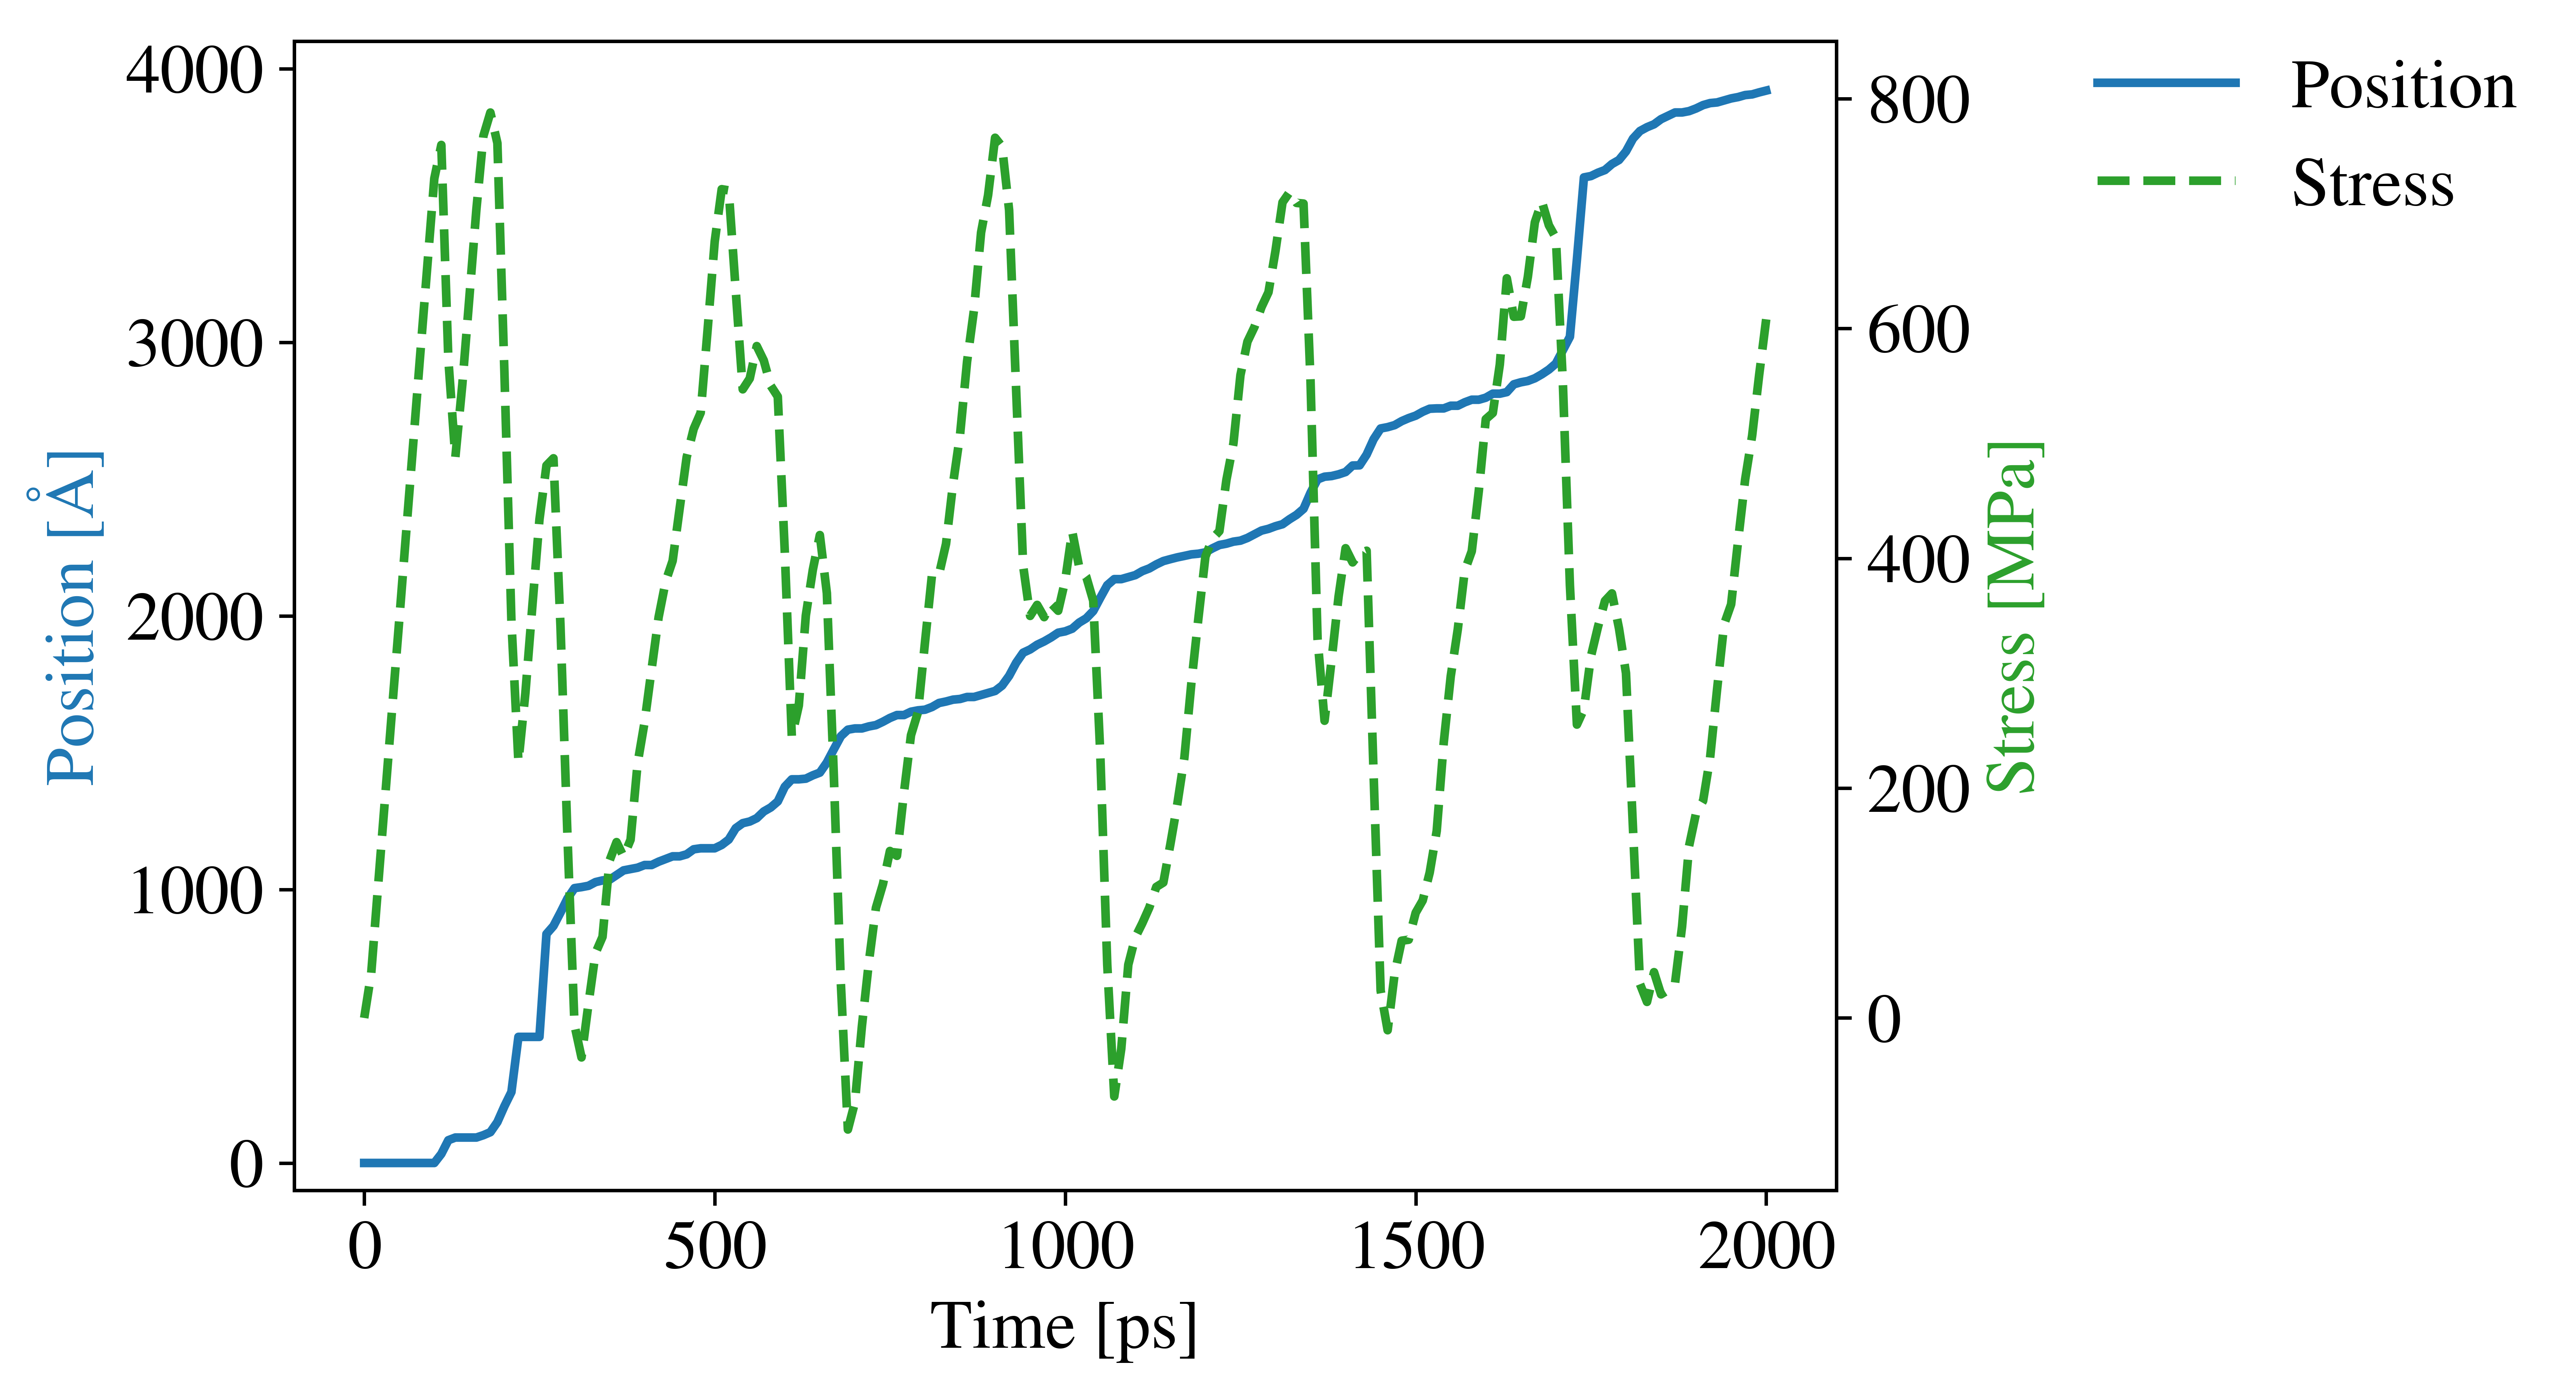
\includegraphics[width=0.6\textwidth]{Position-Stress-ScrewEAM110.png}
    \caption{Movement of the $\frac{1}{2} \langle 110 \rangle \{110\}$ screw dislocation at 1 K under an applied strain rate of $10^{-4}$ s$^{-1}$ as predicted by the Kocevski potential. The average of the developed $\sigma_{yz}$ stress on the dislocation is also shown.}
    \label{Fig:Screw1K}
\end{figure}

The motion of the screw dislocation has been tracked under constant stress in the range of 25--1200 MPa at 300 K, and an example of such calculation is shown in \cref{Fig:Velocity-1000-MPa}. The results of the mobility calculation for the screw dislocation are shown in \cref{Fig:DislocPosTimeScrew}. At stresses smaller than 100 MPa, the screw dislocation oscillates around its initial position without any observable motion. At stresses between 100 and 200 MPa, the screw dislocation performs only a few jumps in the time scale of 1 ns, which results in average velocities in the order of $10^{-1}$ m/s. Between 200 and 700 MPa, motion by the kink-pair mechanism is observed. We fitted \cref{Eq:MobII} to the data points in the 200--700 MPa region and found that $H_0$ = 1.0 eV, $p$ = 0.00037, and $q$ = 0.30. These values have an $R^2$ = 98.3\%. $p$ falls within the expected range of 0--1, although its significantly small value indicates a minor stress dependence. As for the edge dislocation, $q$ is underestimated compared to its expected range of 1--2. $H_0$ for the screw dislocation is larger than that of the edge dislocation (0.11 eV). However, the transition velocity to Regime II, i.e., $v_t$ = 22.1 m/s, is larger than that of the edge dislocation (10.1 m/s) while the transition stress is smaller (700 MPa for the screw dislocation versus 1150 MPa for the edge dislocation). For the stress range 700--1125 MPa, the velocity varies linearly with the stress (Regime II) and values of $M$ = 4546 $\mathrm{Pa}^{-1} \! \cdot \! \mathrm{s}^{-1}$ and $C = - 1134$ m/s fit the data points in this regime to \cref{Eq:MobII} with $R^2$ = 94.8\%. For stresses larger than 1125 MPa, debris production was observed in the wake of the dislocation, which reduced the velocity. The fitting parameters of the screw dislocation mobility function are shown in \cref{Tab:DislocParams}. The linear mobility of the screw dislocation is larger than that of the edge dislocation by more than a factor of 5. Despite the usual caveats expected in comparing the qualitative results of two different interatomic potentials, we can expect based on the results that the screw dislocations most likely dominate the deformation process in UN. This picture agrees with the experimental observation that dislocations in UN are nearly pure screws \cite{Sole1968}.

\begin{figure}[h!]
\centering
\subfloat[]{\label{Fig:DislocMob1S}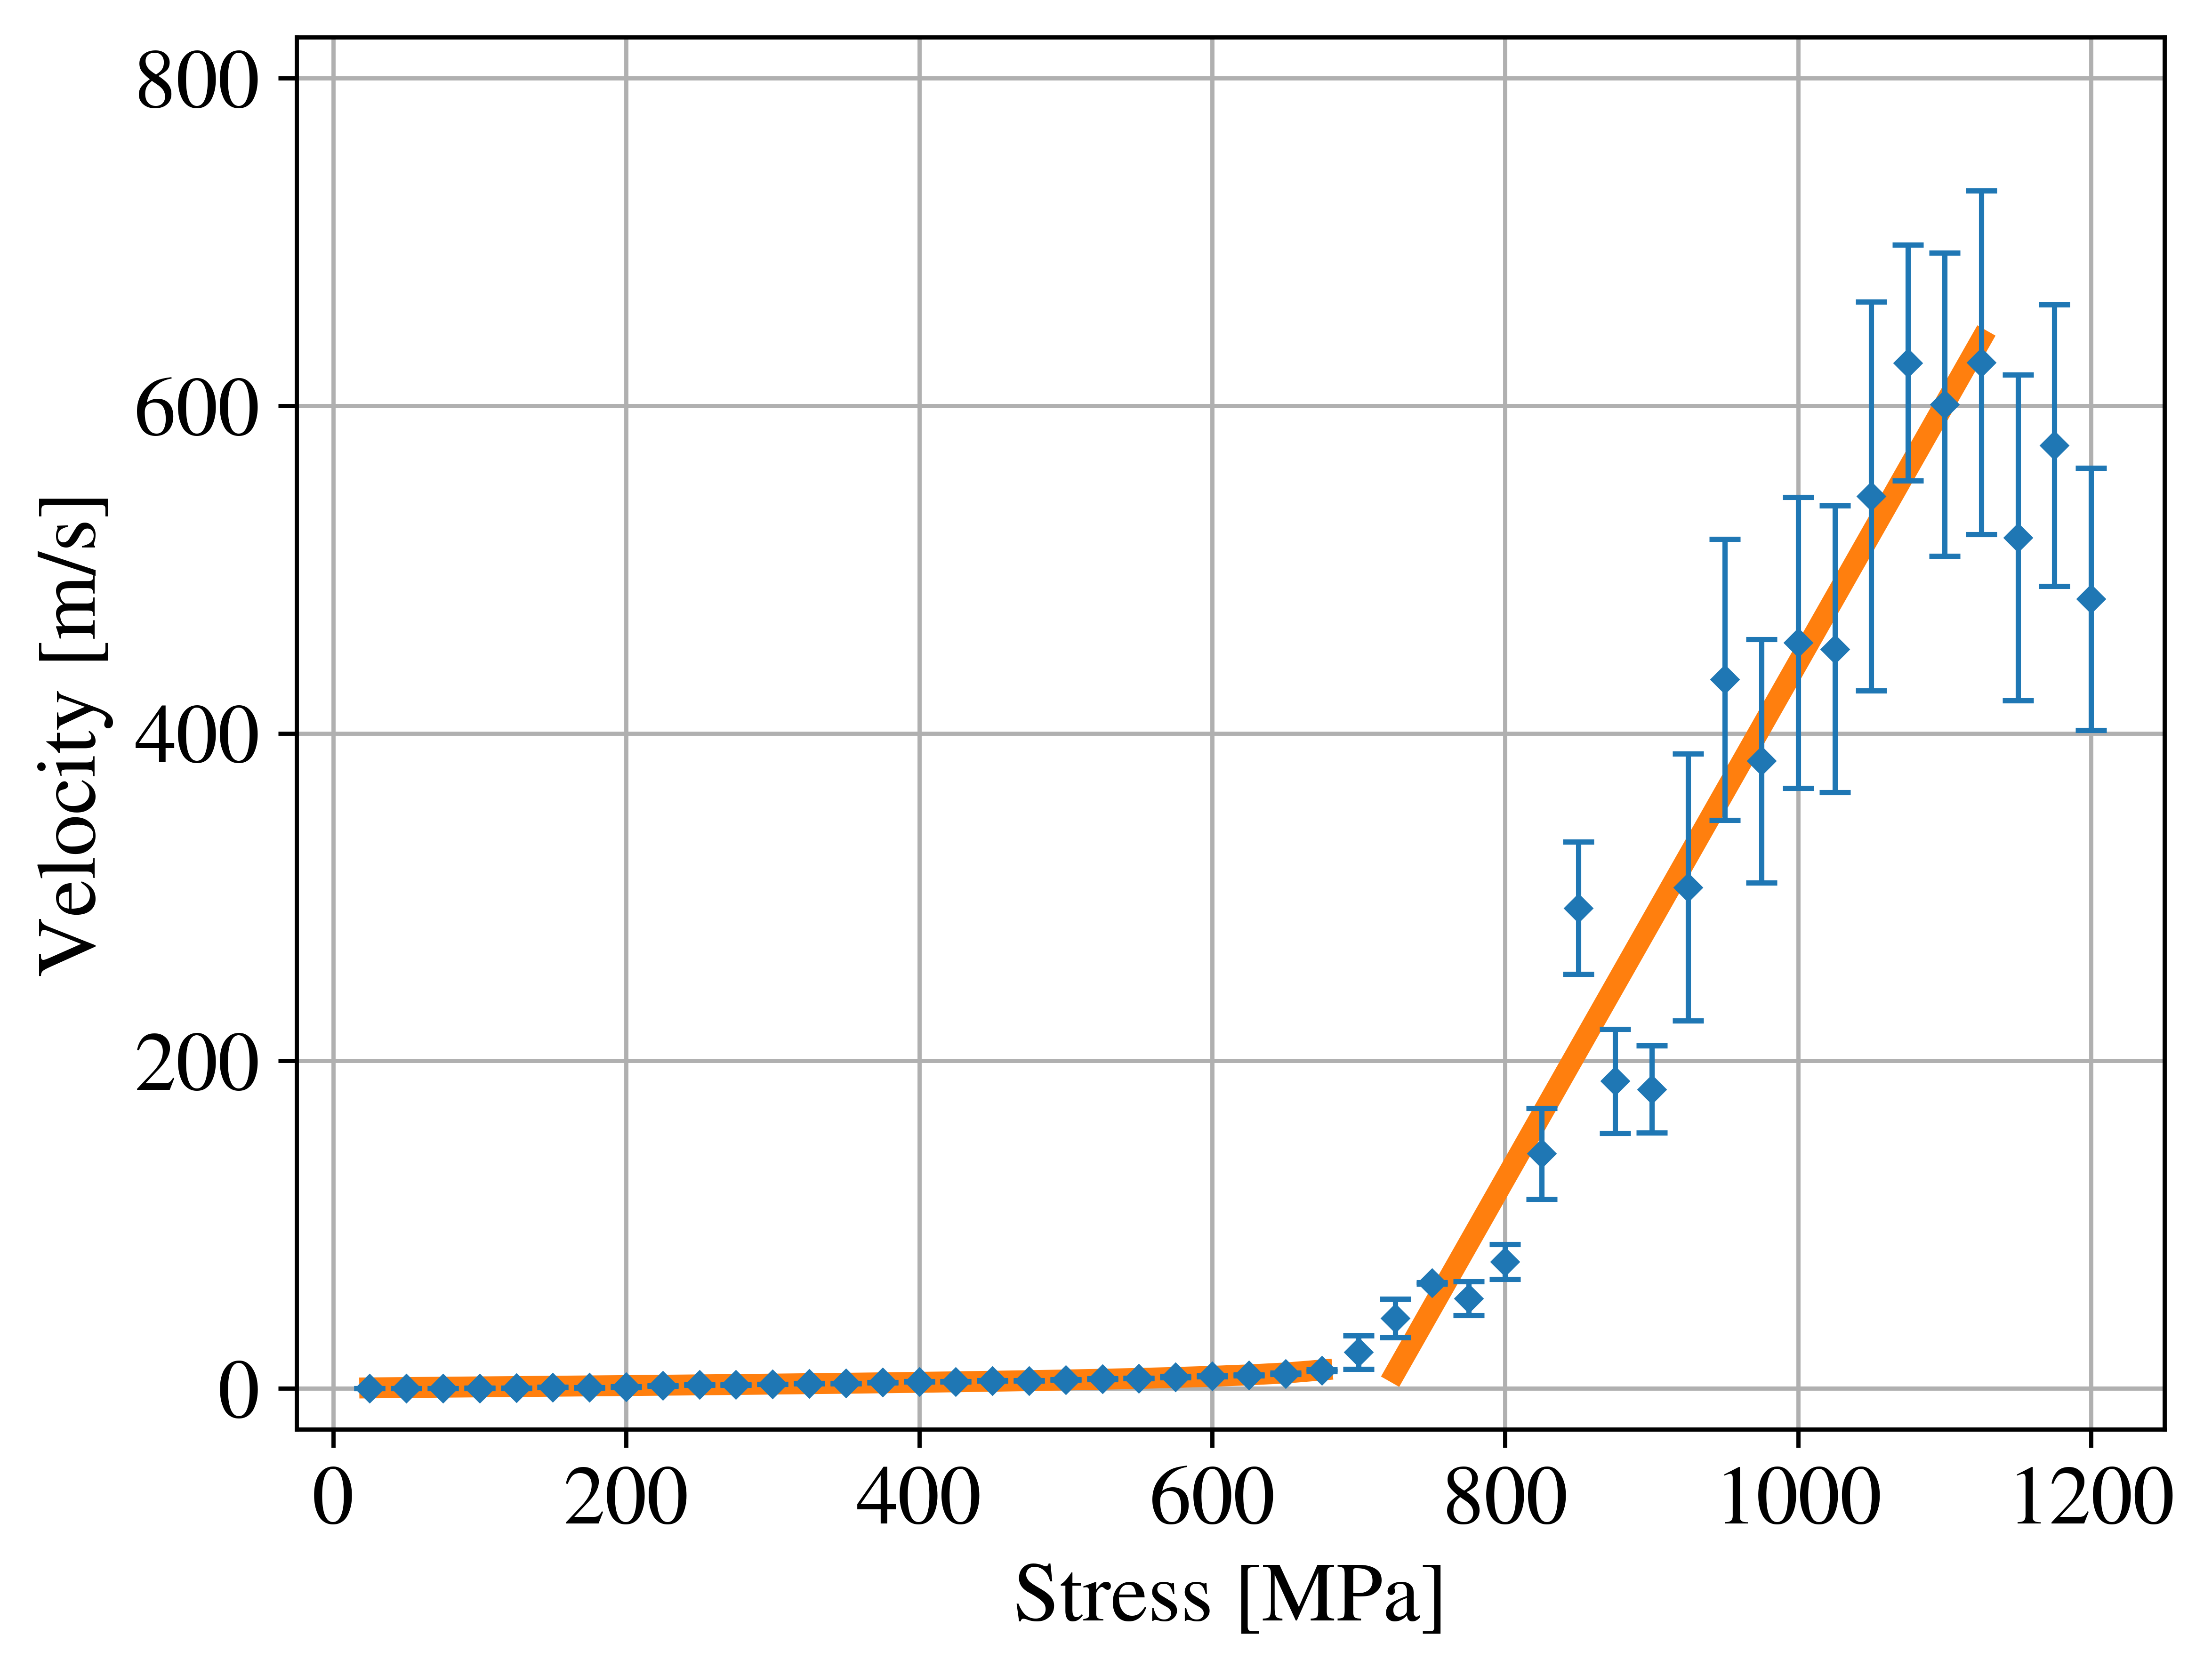
\includegraphics[width=0.48\textwidth]{ScrewMob1.png}}
\hfill
\subfloat[]{\label{Fig:DislocMob2S}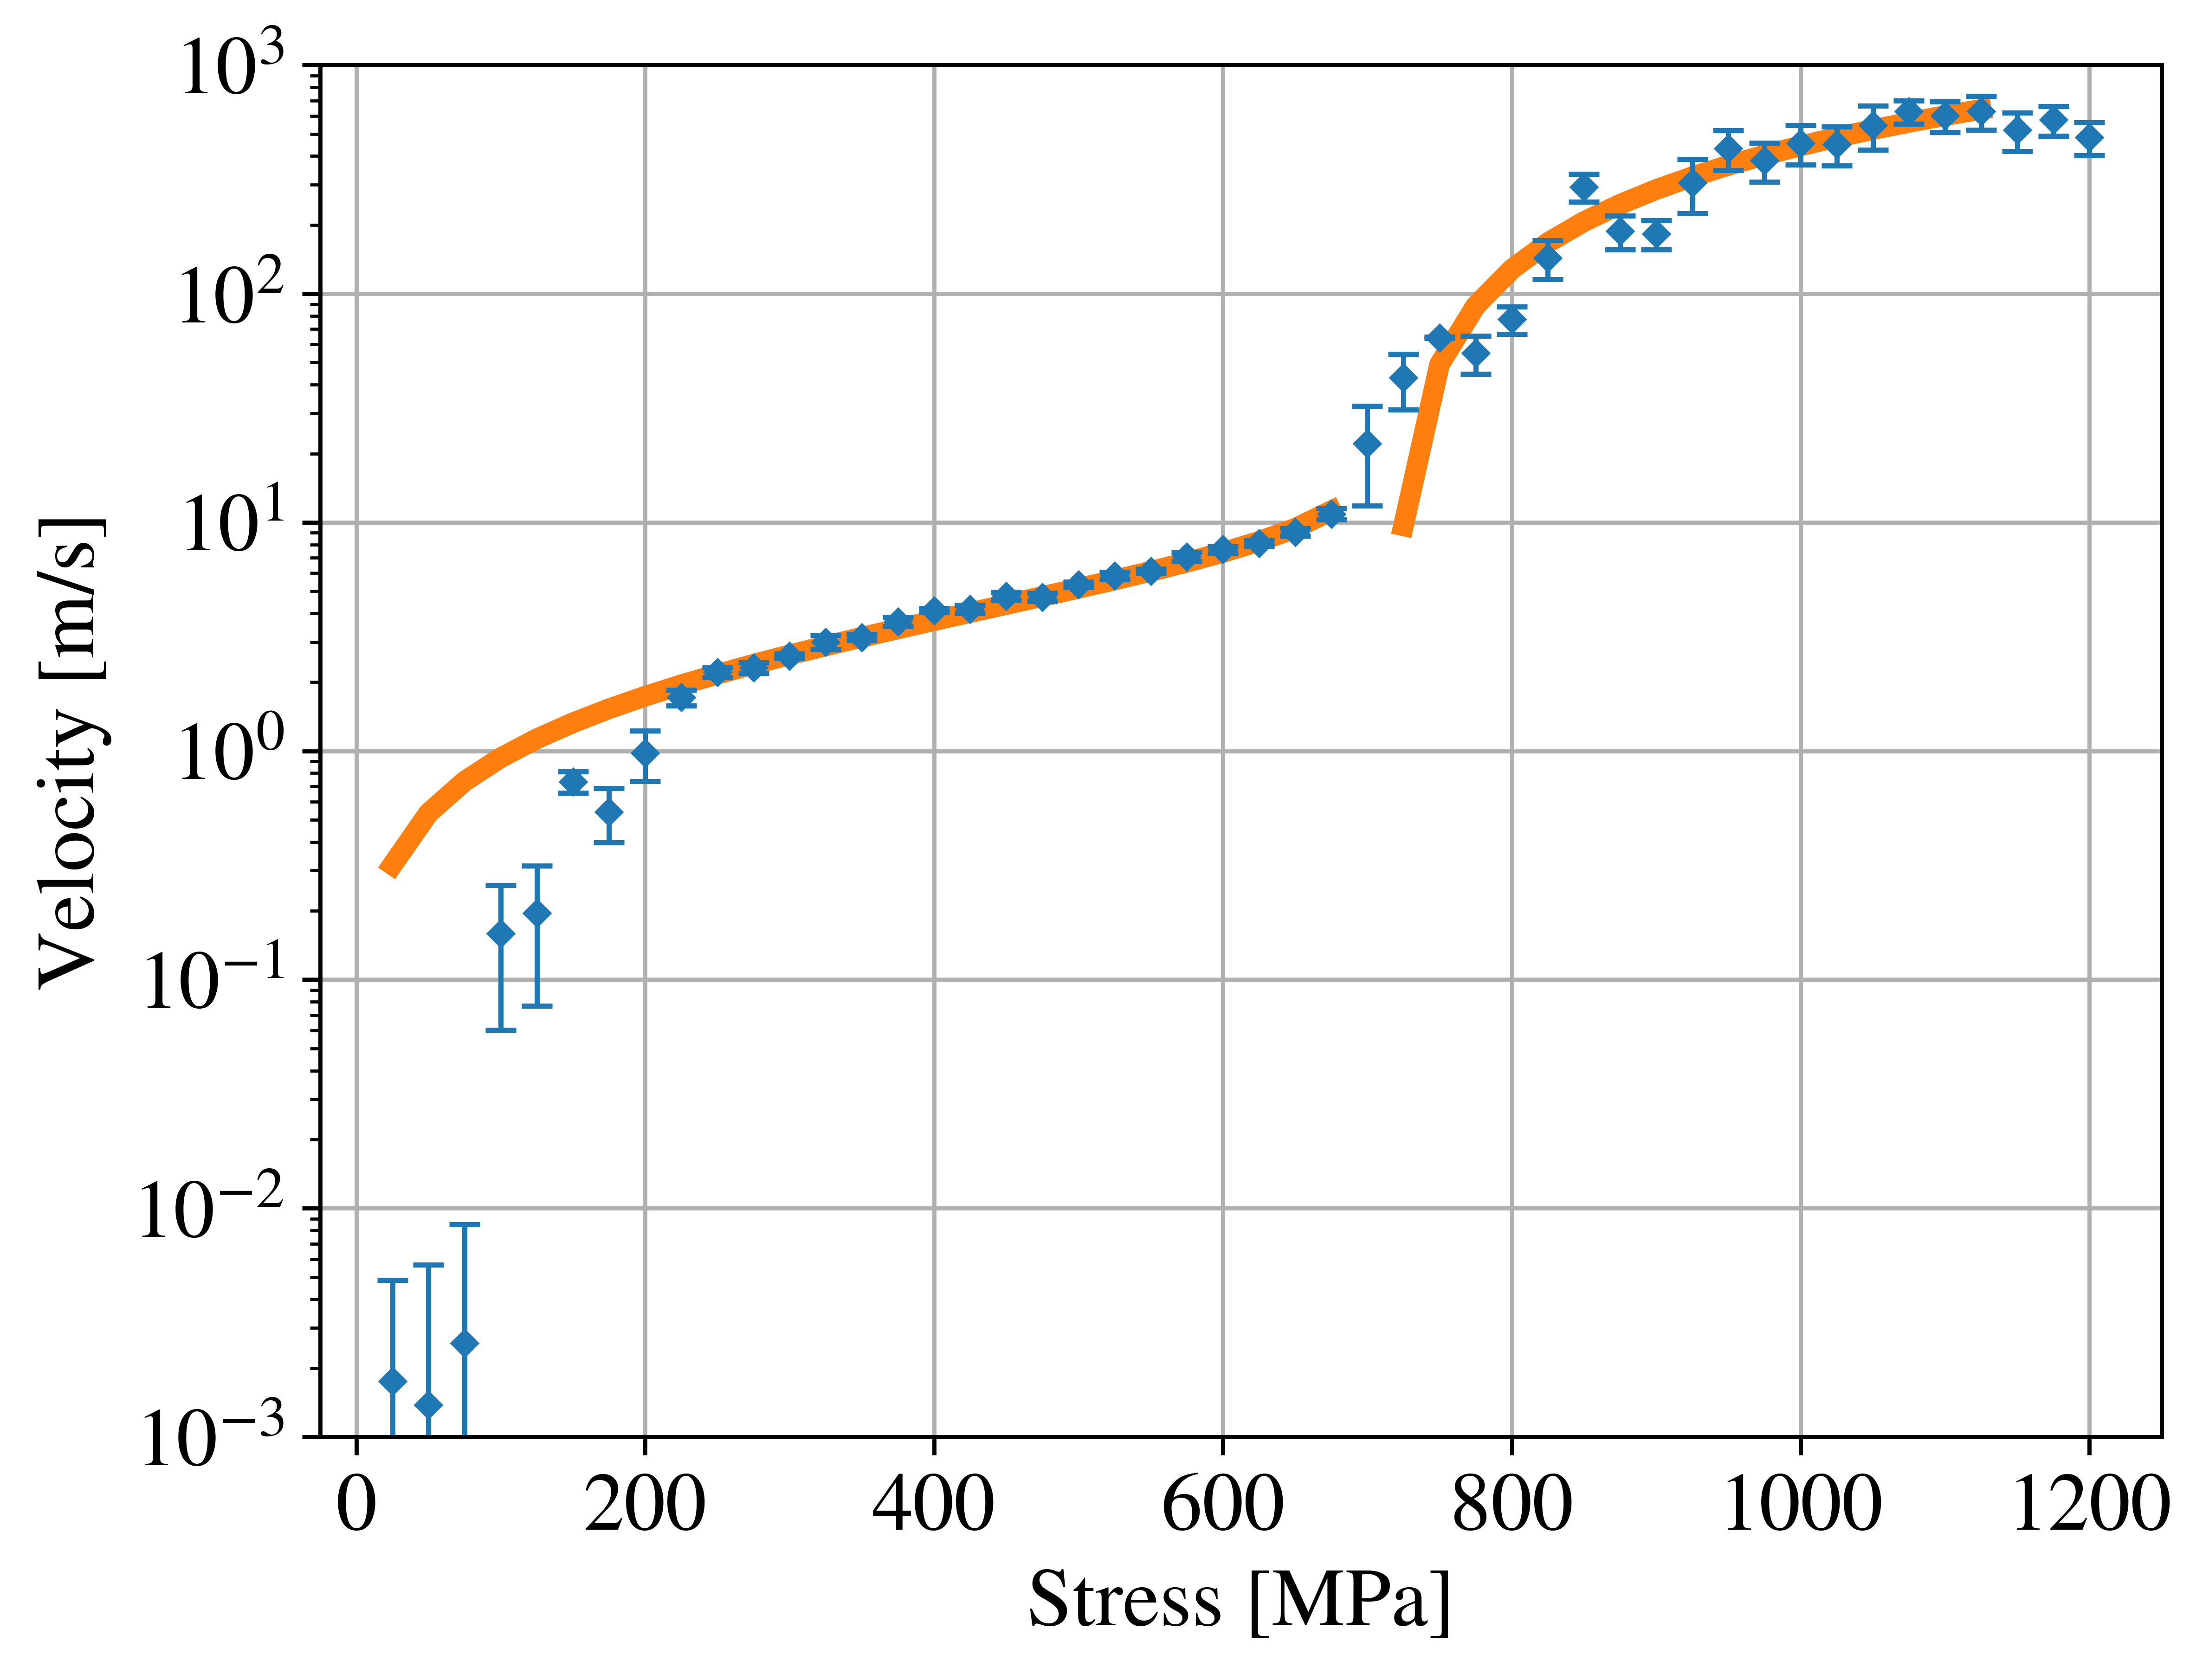
\includegraphics[width=0.48\textwidth]{ScrewMob2.png}}
\caption{The variation of the average screw dislocation velocity in UN with shear stress \textbf{(a)} on a linear scale, and \textbf{(b)} on a semi-log scale. The error bars represent one standard deviation, and the orange lines represent piecewise curve fits.}
\label{Fig:DislocPosTimeScrew}
\end{figure}

\subsubsection{Yield stress estimate}

Based on the definition of the threshold Schmid stress (also known as the critical resolved shear stress (CRSS)), $\tau_S$, as the stress at which the dislocation moves with a velocity of at least 1 m/s \cite{Murty2013}, it is found that for the edge dislocation in UN, $\tau_S$ = 179 MPa, whereas for the screw dislocation, $\tau_S$ = 197 MPa. Although this definition of the CRSS is based on studies on FCC and HCP metals, we assume its validity for UN. According to Stoller and Zinkle \cite{Stoller2000}, an upper-limit estimate of the uniaxial yield stress of a polycrystal can be calculated from:
\begin{equation}
\sigma_y = 3.06 \tau_S
\label{Eq:Taylor}
\end{equation}
which gives $\sigma_y$ = 548--603 MPa. Unlike the GPa-range yield stresses calculated earlier, which are only valid for single-crystal UN, $\sigma_y$ = 548--603 MPa is comparable to the yield stress of macroscopic samples at room temperatures. However, to the best of our knowledge, no experimental stress-strain measurements of UN exist in the open literature.

Another estimate of the yield stress for macroscopic polycrystalline UN can be calculated by the model of Hayes \textit{et al.} \cite{Hayes2004}, which has been used to give a good prediction of the yield stress of $\alpha$-U \cite{Taylor2008}. This model applies the crack formation criterion of brittle fracture \cite{Murty2013} to get a value of the critical stress at which the elastic strain energy imposed upon an elongated single crystal exceeds the surface energy of the crystal. This critical stress correlates with the yield stress because, although UN will fail plastically, its brittle fracture provides a guide to the stress at which the elastic limit is reached. For UN, this critical stress can be calculated as \cite{Hayes2004, Taylor2008}:
\begin{equation}
\sigma_c = 2 \sqrt{\gamma C_{11} / w} 
\end{equation}
where $\gamma$ is the (001) surface energy, $w$ is the sample width, and $C_{11}$ is the elastic constant. According to the DFT study of Bocharov \textit{et al.} \cite{Bocharov2013}, the (001) surface energy is 1.44 J/m$^2$. The sample width, $w$, can be estimated as the size of a 10-$\mu$m single crystal \cite{Hayes2004, Taylor2008}, which is a typical average grain size. The value of $C_{11}$ = 423.9 GPa is taken from experiments \cite{Salleh1986}. Using these values, $\sigma_c$ is about 494 MPa, which agrees within 10\% with the lower limit of the range calculated earlier (i.e., 548 MPa) using \cref{Eq:Taylor}, which is a good agreement considering the widely different approaches used to arrive at the two values. Based on this simple analysis, a rough estimate of the yield stress of UN can be given as 550 MPa.

\section{Discussion}

In this work, we demonstrated that MD simulations can provide accurate predictions of the nanoindentation hardness of UN. We believe this method can be extended to other nuclear fuels, particularly in high-temperature regimes where oxidation layers may limit experimental nanoindentation measurements. The key requirement for an interatomic potential in such simulations is the accurate prediction of the elastic properties and softening behavior. Our findings show that the Kocevski potential gives excellent predictions for nanoindentation hardness, despite its limitations in modeling plasticity dynamics in UN. This is acceptable for simulations where brittle failure dominates, as the plastic deformation dynamics become less relevant. Our earlier work \cite{AbdulHameed2024} has further shown that the Kocevski potential provides a reasonable description of elastic behavior, which is the focus in such brittle regimes.

The Kocevski and Tseplyaev potentials yield different predictions for the principal slip systems in UN. The Kocevski potential predicts that the principal slip system is $\frac{1}{2} \langle 110 \rangle \{110\}$, based on screw dislocation studies, while the Tseplyaev potential suggests $\frac{1}{2} \langle 110 \rangle \{111\}$, as derived from edge dislocation studies. Experimental data \cite{Sole1968} on deformation in UN indicates that the $\{110\}$ planes are the principal slip planes, which aligns with the predictions of the Kocevski potential. This study also noted that screw dislocations are more prevalent in UN \cite{Sole1968}. This experimental observation combined with our finding--that screw dislocations exhibit larger linear mobility and smaller transition stress to the phonon-drag regime compared to edge dislocations--leads us to recommend the screw dislocation mobility function for use in discrete dislocation dynamics (DDD) simulations of UN.

The discrepancy in the predictions of the two potentials may arise from the fact that the Tseplyaev potential likely overestimates the covalent nature of bonding in UN. Another explanation for the differing predictions is that the dominant slip planes in UN may vary with temperature, a phenomenon observed in other materials such as Sr-doped KCl \cite{Haasen1985}. For instance, while $\{111\}$ planes are the primary slip planes in uranium carbide (UC), this conclusion is based on high-temperature measurements (1680–2200 K) \cite{Vasudevamurthy2022}. Since our simulations are conducted at 300 K, further experimental and density functional theory (DFT) studies are required to clarify the principal slip systems in both UN and UC across a range of temperatures.

Dislocation properties, both static and dynamic, are highly sensitive to the chosen interatomic potential. Thus, quantitative conclusions drawn from atomistic models should be considered approximations \cite{Puls1976, Liu2012}. For instance, the Peierls stress of UN, calculated as 2.98 GPa, aligns with the order of magnitude reported for \ce{UO2} by Skelton and Walker, which ranged from 2.7 to 12.9 GPa depending on the interatomic potential used \cite{Skelton2017}. Based on our tests (not shown here), we found that the Peierls stress decreases by approximately 1 GPa when the dislocation line length increases from 40 \AA\ to 80 \AA, though this change does not affect the relative ordering of Peierls stress across the $\frac{1}{2}\langle110\rangle$ slip planes for the edge dislocation. To ensure comparability, it is crucial to evaluate Peierls stress values under consistent simulation conditions, including the same potential, supercell size, and strain rate.

This work presents the first complete mobility functions for $\frac{1}{2}\langle110\rangle$ edge and screw dislocations in UN, providing a foundational step toward parameterizing plasticity dynamics in this material. One limitation of our model is that it is based on simulations at a single temperature (300 K). Key parameters, such as transition stresses and velocities between different regimes, as well as the phonon drag coefficient, are known to vary strongly with temperature \cite{Olmsted2005, Gilbert2011}. For example, transition stresses and velocities between Regimes I and II tend to decrease with increasing temperature, while the phonon drag coefficient typically exhibits an inverse temperature dependence ($B \sim 1/T$). Therefore, future work should involve extending these simulations to higher temperatures to analyze the trends in these parameters. Additionally, our atomistic simulations neglect dislocation-dislocation interactions, meaning the mobility function we present here represents an upper limit at 300 K. However, since the Tseplyaev potential treats UN plasticity as that of a purely covalent material, it may underestimate dislocation mobility, leading to a partial cancellation of errors between these two factors. Thus, the edge dislocation mobility function presented here is expected to be a reasonable estimate. 

% It should also be noted that the dislocation mobility functions we derived are not continuous at the transition stress. For numerical implementation in a DDD code, both the mobility function and its first derivative must be continuous. This can be achieved by performing ``curve stitching'' between the piecewise functions to ensure smoothness, a task left for future studies. Open-source DDD codes, such as ParaDiS \cite{Arsenlis2007}, can be extended to incorporate complex mobility functions like those presented here. For instance, Starikov and Tseplyaev \cite{Starikov2020} implemented a custom mobility function for molybdenum. Such an extension could be similarly implemented for UN using the mobility functions developed in this work.

The estimated threshold Schmid stress for dislocation glide in UN (179--197 MPa) and the corresponding uniaxial yield stress (548--603 MPa) represent upper-limit estimates. This is primarily due to our use of the Taylor factor (3.06) in calculating these values, which could be lower in real materials due to factors such as texture \cite{Stoller2000}. Nevertheless, the yield stress predicted by our crack formation criterion (494 MPa) lends confidence to our estimates. An average yield stress of approximately 550 MPa is reasonable based on our findings, and we recommend its use as an input parameter in future plasticity or dislocation dynamics models until experimental data is available.

\section{Conclusions}

In this study, we employed MD simulations to investigate specific aspects of the mechanical behavior of UN. First, we analyze the deformation behavior in nanometer-sized UN single-crystals. The Kocevski potential predicted the principal slip system as $\frac{1}{2} \langle 110 \rangle \{110\}$, aligning with experimental data, while the Tseplyaev potential predicted slip on $\frac{1}{2} \langle 110 \rangle \{111\}$. The study demonstrates that MD simulations of stress-strain curves in single crystals with free surfaces yield accurate estimates of the nanoindentation hardness of UN. Nanoindentation hardness was accurately predicted by the Kocevski potential, though it struggled to model dynamic plasticity. This methodology is particularly advantageous at elevated temperatures, where oxidation hinders direct measurements of UN's nanoindentation hardness. Further exploration involved the determination of the Peierls stress for the $\frac{1}{2} \langle 110 \rangle$ edge dislocation along the $\{ 110 \}$, $\{ 111 \}$, and $\{ 112 \}$ slip planes and for the $\frac{1}{2} \langle 110 \rangle$ screw dislocation along $\{110\}$. The $\{ 111 \}$ plane displayed the smallest value (2.98 GPa) agreeing with the results of the stress-strain behavior predicted by the Tseplyaev potential. For the screw dislocation, the Peierls stress is determined to be about 790 MPa using the Kocevski potential. Both edge and screw dislocations are found to move via the kink-pair nucleation mechanism before displaying a linear variation of their velocity with stress. Based on these results, complete dislocation mobility functions were fitted and the linear mobility is found to be 817 $\mathrm{Pa}^{-1} \! \cdot \! \mathrm{s}^{-1}$ for the edge dislocation using the Tseplyaev potential, and 4546 $\mathrm{Pa}^{-1} \! \cdot \! \mathrm{s}^{-1}$ for the screw dislocation using the Kocevski potential. The threshold Schmid stress was estimated between 179 and 197 MPa, corresponding to an upper-limit uniaxial yield stress of 548–603 MPa for polycrystalline UN. These values show the expected orders of magnitude and can be used as inputs for plasticity or dislocation dynamics models. Finally, we observed that, at intermediate stresses, the subsonic steady-state motion of the edge dislocation in UN can be interrupted by jumps that have a maximum velocity equal to the average sound velocity.

To the best of our knowledge, this study is the first computational investigation of the stress-strain behavior and dislocation properties in UN, and the first that attempts to fit complete mobility functions for dislocations in a nuclear fuel. We believe this work provides a baseline for the computational study of dislocations in nuclear fuels that can be expanded and built upon by, e.g., conducting the analysis at higher temperatures which are more relevant for the operational conditions of nuclear reactors.

\vspace{6pt}

% Optional
% \supplementary{The following supporting information can be downloaded at: \linksupplementary{s1}, Figure S1: title; Table S1: title; Video S1: title.}

% Only used for preprints:
% \supplementary{The following supporting information can be downloaded at the website of this paper posted on \href{https://www.preprints.org/}{Preprints.org}.}

\authorcontributions{Conceptualization, M.A., B.B. and A.C.; methodology, M.A.; formal analysis, M.A.; writing---original draft preparation, M.A..; writing---review and editing, M.A. and B.B.; visualization, M.A.; project administration, B.B.; funding acquisition, A.C. All authors have read and agreed to the published version of the manuscript.}

\funding{This research was funded by the Westinghouse Electric Company.}

\dataavailability{Research data can be made available upon request.} 

\acknowledgments{The authors would like to thank Michael W.D. Cooper, Conor O.T. Galvin, Mahmoud Hawary, and Shehab Shousha for the fruitful discussions and useful suggestions. This research made use of the resources of the High-Performance Computing Center at Idaho National Laboratory, which is supported by the Office of Nuclear Energy of the U.S. Department of Energy and the Nuclear Science User Facilities under Contract No. DE-AC07-05ID14517. Mohamed AbdulHameed dedicates this work to the memory of Ammar Alkhowesky.}

\conflictsofinterest{The authors declare no conflicts of interest.} 



% Optional
% \appendixtitles{no} % Leave argument "no" if all appendix headings stay EMPTY (then no dot is printed after "Appendix A"). If the appendix sections contain a heading then change the argument to "yes".
% \appendixstart
% \appendix
% \section[\appendixname~\thesection]{}
% \subsection[\appendixname~\thesubsection]{}
% The appendix is an optional section that can contain details and data supplemental to the main text---for example, explanations of experimental details that would disrupt the flow of the main text but nonetheless remain crucial to understanding and reproducing the research shown; figures of replicates for experiments of which representative data are shown in the main text can be added here if brief, or as Supplementary Data. Mathematical proofs of results not central to the paper can be added as an appendix.

% \section[\appendixname~\thesection]{}
% All appendix sections must be cited in the main text. In the appendices, Figures, Tables, etc. should be labeled, starting with ``A''---e.g., Figure A1, Figure A2, etc.

% \isPreprints{}  % If the paper is ``preprints'', please uncomment this parenthesis.
%\printendnotes[custom] % Un-comment to print a list of endnotes

\reftitle{References}

\bibliography{ref.bib}

\PublishersNote{}

% \isPreprints{} % If the paper is ``preprints'', please uncomment this parenthesis.
\end{document}

